\documentclass[letterpaper]{article}
\usepackage[margin=1in]{geometry}
\usepackage[utf8]{inputenc}
\usepackage{textcomp}
\usepackage{amssymb}
\usepackage{natbib}
\usepackage{graphicx}
\usepackage{gensymb}
\usepackage{amsthm, amsmath, mathtools}
\usepackage[dvipsnames]{xcolor}
\usepackage{enumerate}
\usepackage{mdframed}
\usepackage[most]{tcolorbox}
\usepackage{csquotes}
% https://tex.stackexchange.com/questions/13506/how-to-continue-the-framed-text-box-on-multiple-pages

\tcbuselibrary{theorems}

\newcommand{\R}{\mathbb{R}}
\newcommand{\Z}{\mathbb{Z}}
\newcommand{\N}{\mathbb{N}}
\newcommand{\Q}{\mathbb{Q}}
\newcommand{\C}{\mathbb{C}}
\newcommand{\code}[1]{\texttt{#1}}
\newcommand{\mdiamond}{$\diamondsuit$}
\newcommand{\PowerSet}{\mathcal{P}}
\newcommand{\Mod}[1]{\ (\mathrm{mod}\ #1)}
\DeclareMathOperator{\lcm}{lcm}

%\newtheorem*{theorem}{Theorem}
%\newtheorem*{definition}{Definition}
%\newtheorem*{corollary}{Corollary}
%\newtheorem*{lemma}{Lemma}
\newtheorem*{proposition}{Proposition}


\newtcbtheorem[number within=section]{theorem}{Theorem}
{colback=green!5,colframe=green!35!black,fonttitle=\bfseries}{th}

\newtcbtheorem[number within=section]{definition}{Definition}
{colback=blue!5,colframe=blue!35!black,fonttitle=\bfseries}{def}

\newtcbtheorem[number within=section]{corollary}{Corollary}
{colback=yellow!5,colframe=yellow!35!black,fonttitle=\bfseries}{cor}

\newtcbtheorem[number within=section]{lemma}{Lemma}
{colback=red!5,colframe=red!35!black,fonttitle=\bfseries}{lem}

\newtcbtheorem[number within=section]{example}{Example}
{colback=white!5,colframe=white!35!black,fonttitle=\bfseries}{def}

\newtcbtheorem[number within=section]{note}{Important Note}{
        enhanced,
        sharp corners,
        attach boxed title to top left={
            xshift=-1mm,
            yshift=-5mm,
            yshifttext=-1mm
        },
        top=1.5em,
        colback=white,
        colframe=black,
        fonttitle=\bfseries,
        boxed title style={
            sharp corners,
            size=small,
            colback=red!75!black,
            colframe=red!75!black,
        } 
    }{impnote}
\usepackage[utf8]{inputenc}
\usepackage[english]{babel}
\usepackage{fancyhdr}
\usepackage[hidelinks]{hyperref}

\pagestyle{fancy}
\fancyhf{}
\rhead{CSE 101}
\chead{March 15th, 2021}
\lhead{Course Notes}
\rfoot{\thepage}

\setlength{\parindent}{0pt}

\begin{document}

\begin{titlepage}
    \begin{center}
        \vspace*{1cm}
            
        \Huge
        \textbf{CSE 101}
            
        \vspace{0.5cm}
        \LARGE
        Design and Analysis of Algorithms
            
        \vspace{1.5cm}
            
        \vfill
            
        Winter 2022 \\
        Taught by Professor Daniel Kane
    \end{center}
\end{titlepage}

\pagenumbering{gobble}

\newpage 

\pagenumbering{gobble}
\begingroup
    \renewcommand\contentsname{Table of Contents}
    \tableofcontents
\endgroup

\newpage
\pagenumbering{arabic}

\section{Introduction to Algorithms}
In this class, we'll talk about algorithms. To start this class off, we'll consider the Fibonacci Numbers. 

\subsection{Problem: Fibonacci Numbers}
\begin{definition}{Fibonacci Numbers}{}
    The \textbf{Fibonacci numbers} are the sequence defined by: 
    \[F_0 = F_1 = 1\]
    \[F_n = F_{n - 1} + F_{n - 2} \text{ for } n \geq 2\]
\end{definition}

\subsubsection{Naive Algorithm}
There is an easy recursive algorithm:
\begin{verbatim}
    Fib(n)
        if n <= 1
            Return 1
        Else 
            Return Fib(n - 1) + Fib(n - 2)
\end{verbatim}

\subsubsection{Runtime}
Let $T(n)$ be the number of lines of code $\code{Fib}(n)$ needs to execute.
\begin{itemize}
    \item The \code{if} and \code{else} statements make up 2 lines of code. 
    \item Otherwise, we need to run $1 + T(n - 1) + T(n - 2)$ lines.
\end{itemize}
So: 
\[T(n) = \begin{cases}
    2 & n \leq 1 \\ 
    T(n - 1) + T(n - 2) + 3 & \text{Otherwise}
\end{cases}\]
Here, if we want to compute $\code{Fib}(100)$, the runtime would be: 
\[T(100) \approx 2.87 \cdot 10^{21}\]
At a billion lines of code per second, this would take over 90,000 years to run. 

\subsubsection{Why So Slow?}
This algorithm, in particular, has too many (redundant) recursive calls. For example:
\[f(5) = f(4) + f(3)\]
\[f(4) = f(3) + f(2)\]
\[f(3) = f(2) + f(1)\]
Already, there are some repeated calls. How can we make this more efficient? 

\subsubsection{Improving this Algorithm}
First, we avoid recomputing things. When we do this by hand, we often already have the last two numbers. So, we can use an array to store the $n$th Fibonacci number. 

\subsubsection{Improved Algorithm}
If we were to simulate finding the Fibonacci numbers by hand, we would have an algorithm similar to:
\begin{verbatim}
    Fib2(n)
        Initialize A[0..n]
        A[0] = A[1] = 1
        For k = 2 to n
            A[k] = A[k - 1] + A[k - 2]
        Return A[n]
\end{verbatim}
In the first two lines (initializing the array and setting initial values), there are 2 lines. In the \code{for} loop, we run $2(n - 1)$ lines. Finally, we run 1 line of code. So, we have the final result of: 
\[T(n) = 2n + 1\]
With this new algorithm, we have $T(100) = 201$. So, this is easily runnable on almost any computer.

\bigskip 

Essentially, the power of algorithms is: 
\begin{mdframed}
    Sometimes, the right algorithm is the difference between something working and not finishing in your lifetime. 
\end{mdframed}

\subsection{Levels of Algorithm Design}
In this class, there are several things we consider when designing algorithms. 
\begin{itemize}
    \item \textbf{Naive Algorithms:} Turn definition into algorithm. This is easy to wirte, good first pass, but often very slow. Good way to ``test.''
    \item \textbf{Toolkit:} Algorithms designed using standard tools the main focus of this course. 
    \item \textbf{Optimized:} Use data structures or other ideas to make algorithm especially efficient. 
    \item \textbf{Magic:} Sometimes, an algorithm requires a surprising new insight. 
\end{itemize}




















\newpage 
\section{Undirected Graph Algorithms}
\begin{definition}{Graph}{}
    A \textbf{graph} $G = (V, E)$ consists of two things:
    \begin{itemize}
        \item A collection $V$ of vertices, or objects to be connected.
        \item A collection $E$ of edges, each of which connects a pair of vertices.
    \end{itemize}
\end{definition}

For example, we can model the following as graphs: 
\begin{itemize}
    \item The internet, where $V$ is the websites and $E$ are links. 
    \item The internet, where $V$ are computers and $E$ are physical connections. 
    \item A highway system, where $V$ are the intersections and $E$ are the roads. 
\end{itemize}
In computer science, there are a few examples of graphs: 
\begin{itemize}
    \item The internet (webpages, physical connections, etc.)
    \item Social networks (especially with friendship, connections).
    \item Transitions between states of a program. 
    \item Road maps. 
\end{itemize}
Another question we might ask is, how do you store a graph in a computer?
\begin{itemize}
    \item \textbf{Adjacency Matrix:} Store list of vertices and an array \code{A[i, j] = 1} if edge between $v_i$ and $v_j$.
    \begin{itemize}
        \item Slow space for dense graphs.
        \item Slow for most operations.
    \end{itemize}

    \item \textbf{Edge List:} List of all vertices with list of all edges. 
    \begin{itemize}
        \item More space-efficient for a sparse graph. 
        \item Hard to determine edges outof the single vertex.
    \end{itemize}

    \item \textbf{Adjacency List:} For each vertex, store a list of neighbors.
    \begin{itemize}
        \item Needed for DFS to be efficient. 
        \item We will usually assume this representation.
    \end{itemize}
\end{itemize}

\subsection{Drawing Graphs}
When drawing graphs, we want to draw the vertices first. Then, for each edge, draw line segments or curves connecting those points. 
\begin{center}
    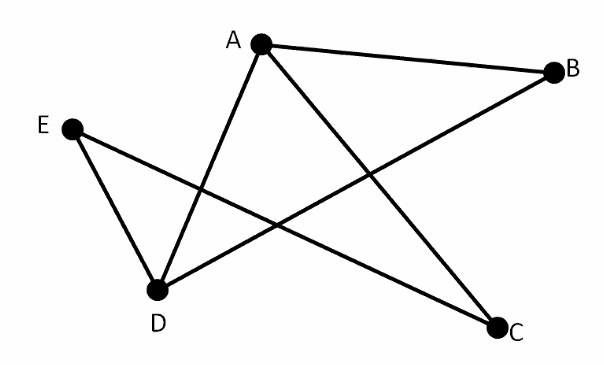
\includegraphics[scale=0.5]{assets/graph.png}
\end{center}
This particular graph can be represented by $G = (V, E)$ where: 
\[V = \{A, B, C, D, E\}\]
\[E = \{(A, B), (A, C), (A, D), (B, D), (C, E), (D, E)\}\]
Because this is an \underline{unordered} graph, $(A, B)$ and $(B, A)$ mean the same thing. 

\subsection{Problem: Exploring Graphs}
Suppose we are playing a video game and want to make sure that you've found all the areas in this level before moving on to the next one. How do we ensure that we found everything? 

\subsubsection{Basic Algorithm}
Essentially, we want to: 
\begin{verbatim}
    Keep track of all areas discovered.
    While there is an unexplored path:
        Follow path. 
\end{verbatim}

\subsubsection{Systematize}
Essentially, we need to keep track of: 
\begin{itemize}
    \item Which vertices we have discovered. 
    \item Which edges have yet to be explored.
\end{itemize}
So, the explore algorithm will:
\begin{itemize}
    \item Use a field \code{v.visted} to let us know which vertices we have seen.
    \item Store edges to be explored implicitly in the program stack. 
\end{itemize}

\begin{verbatim}
    explore(v):
        v.visited <- true 
        for each edge (v, w):
            if not w.visited:
                explore(w)
                w.prev <- v     // If we want to keep track of path taken
\end{verbatim}

\subsubsection{Result}
\begin{theorem}{}{}
    If all vertices start unvisited, \code{explore(v)} marks as visited exactly the vertices reachable from \code{v}.
\end{theorem}

\begin{mdframed}[]
    \begin{proof}
        First, we note that we can only visit vertices that are reachable from $v$. If $u$ is visited, then eventally we will visit every adjacent $w$. If there is a chain of vertices, then $v$ will visit $u_1$ which will visit $u_2$ which will visit everything up to and including $w$. 
    \end{proof}
\end{mdframed}

\subsection{Problem: Depth First Search}
\code{explore} only finds the part of the graph reachable from a single vertex. If you want to discover the entire graph, you may need to run it multiple times. This introduces an algorithm known as \textbf{depth first search}:
\begin{verbatim}
    DepthFirstSearch(v):
        Mark all v in G as unvisited. 
        For v in G:
            if not v.visited:
                explore(v)
\end{verbatim}
Here, this runs in $O(|V|)$ time: we need to iterate over vertex. 

\subsubsection{Runtime of DFS}
\begin{verbatim}
    explore(v):                 // Run once per vertex O(|V|) 
        v.visited <- true       // Run once per vertex 
        for each edge (v, w):   // Run once per neighboring vertex O(|E|)
            if not w.visited:   // Run once per neighboring vertex
                explore(w)      // Run once per neighboring vertex
                w.prev <- v     // Run once per neighboring vertex
\end{verbatim}
So, our final runtime is: 
\[O(2|V| + |E|) = O(|V| + |E|)\]
Although $O(|V| + |E|)$ is linear time, in reality, graph algorithm runtimes depend on both $|V|$ and $|E|$. What algorithm is better may depend on the relative sizes of these parameters.

\begin{center}
    \begin{tabular}{c|c|c}
                & \textbf{Sparse Graphs} & \textbf{Dense Graphs} \\ 
        \hline
        Runtime & $|E|$ small ($\approx V$) & $|E|$ large ($\approx V^2$) \\ 
        Examples & Internet, Road Maps & Flight Maps, Wireless Networks 
    \end{tabular}
\end{center}


\subsection{Problem: Connected Components}
We want to understand which vertices are reachable from which others in a graph. We've already kind of done this using \code{explore(v)} to find which vertices are reachable from a given vertex. 

\bigskip 

For a more theoretical answer, consider the theorem: 
\begin{theorem}{}{}
    The vertices of a graph $G$ can be partitioned into connected components so that $v$ is is reachable from $w$ if and only if they are in the same connected component. 
\end{theorem}

For instance, consider the following graph:
\begin{center}
    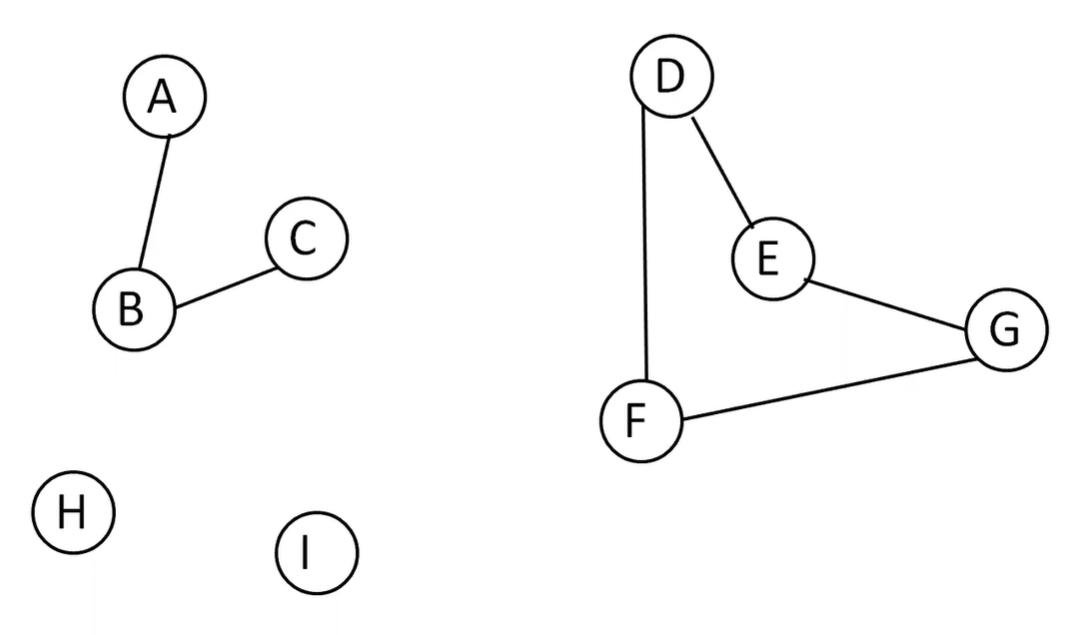
\includegraphics[scale=0.35]{assets/graph_con.png}
\end{center}
We can split this graph into four components: 
\begin{center}
    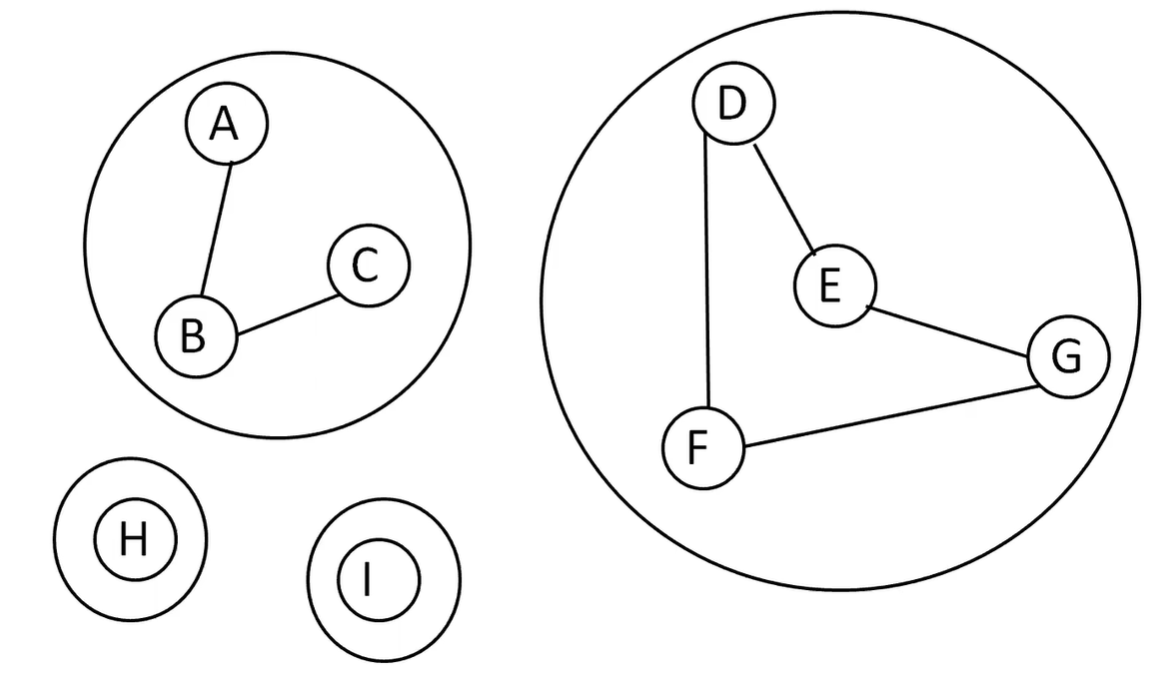
\includegraphics[scale=0.35]{assets/graph_con_2.png}
\end{center}
Here, if there are two points in a component, then we can reach the first point from the second and vice versa. However, if there are two points in two different components, then this is not possible.  

\bigskip 

\textbf{Problem Statement:} Given a graph $G$, how do we compute its connected components? 
\begin{itemize}
    \item \underline{Easy Way:} For each $v$, run \code{explore(v)} to find the vertices reachable from it. Group together into components. The runtime will be $O(|V|(|V| + |E|))$. 
    \item \underline{Better Way:} Run \code{explore(v)} to find the components of $v$. Then, repeat this on the unclassified vertices. 
\end{itemize}

\subsubsection{Applying Depth-First Search (DFS)}
We can use depth-first search to simulate this. In fact, we can use the same algorithm above but with a bit of additional ``information'' to get our answer:
\begin{verbatim}
    explore(v, CCNum):
        v.visited = true 
        // CC is connected components
        v.CC = CCNum 
        for each edge (v, w):
            if not w.visited: 
                explore(w)

    ConnectedComponents(G):
        CCNum = 0
        for each v in G:
            v.visited = false
        for each v in G: 
            if not v.visited: 
                CCNum++
                explore(v, CCNum)
\end{verbatim}
The runtime is $O(|V| + |E|)$. 

\bigskip

If we recall the graph above, running this algorithm would yield something like:
\begin{center}
    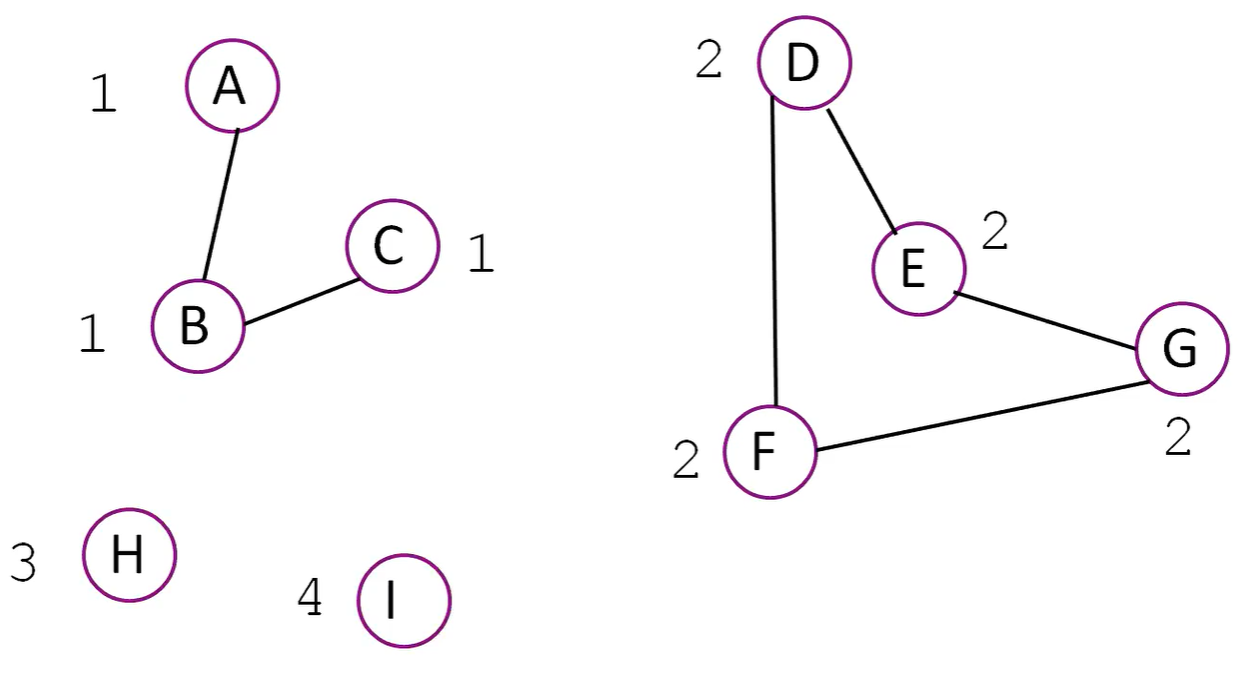
\includegraphics[scale=0.35]{assets/graph_con_3.png}
\end{center}
Where \code{CCNum} is \code{4}, or 4 connected components. 


\subsubsection{DFS: A Discussion}
What does DFS actually do? 
\begin{itemize}
    \item No output.
    \item Marks all vertices as visited. 
    \item Easier ways to do it.
\end{itemize}
However, DFS is a useful way to \emph{explore the graph}. In particular, by augmenting the algorithm a bit, like we did with the connected components algorithm, we can learn useful things. In other words, DFS by itself is quite useless, but adding a bit of additional information will make it more useful. 

\subsubsection{Pre- and Post- Order}
How can we augment this algorithm?
\begin{itemize}
    \item Keep track of what algorithm does and in what order. 
    \item Have a ``clock'' and note time whenever: 
    \begin{itemize}
        \item Algorithm visits a new vertex for the first time. 
        \item Algorithm finishes processing a vertex.
    \end{itemize}
    \item Finally, we can record values as \code{v.pre} and \code{v.post}.
\end{itemize}

\subsubsection{Computing Pre- and Post- Order}
Consider the algorithm, which is the same thing as above but with some changes to make it useful: 
\begin{verbatim}
    explore(v)
        v.visited = true 
        v.pre = clock 
        clock++
        For each edge (v, w)
            If not w.visited
                explore(w)
        v.post = clock 
        clock++

    DepthFirstSearch(G)
        clock = 1
        Mark all v in G as unvisited
        For v in G
            If not v.visited
                explore(v)
\end{verbatim}
The runtime is still $O(|V| + |E|)$. 

\subsubsection{Example of Pre- and Post- Order}
Consider the following graph:
\begin{center}
    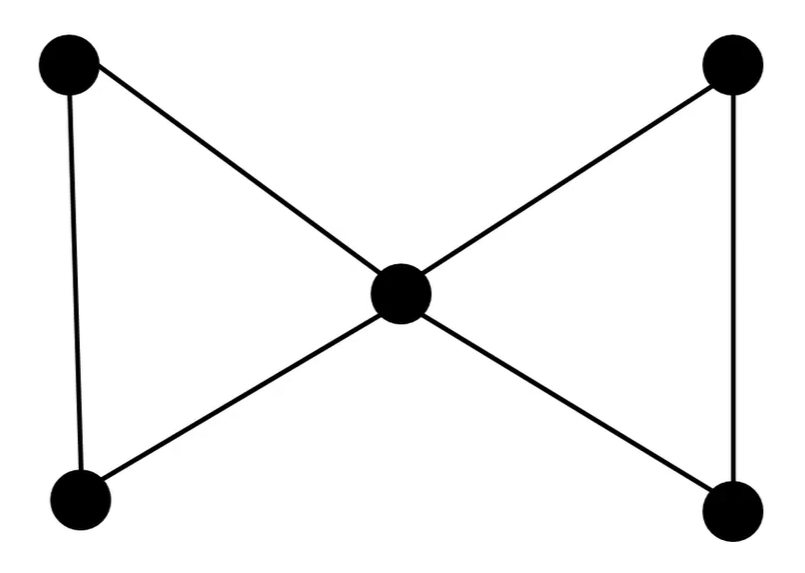
\includegraphics[scale=0.3]{assets/graph_tri.png}
\end{center}
After running the above algorithm, we get:
\begin{center}
    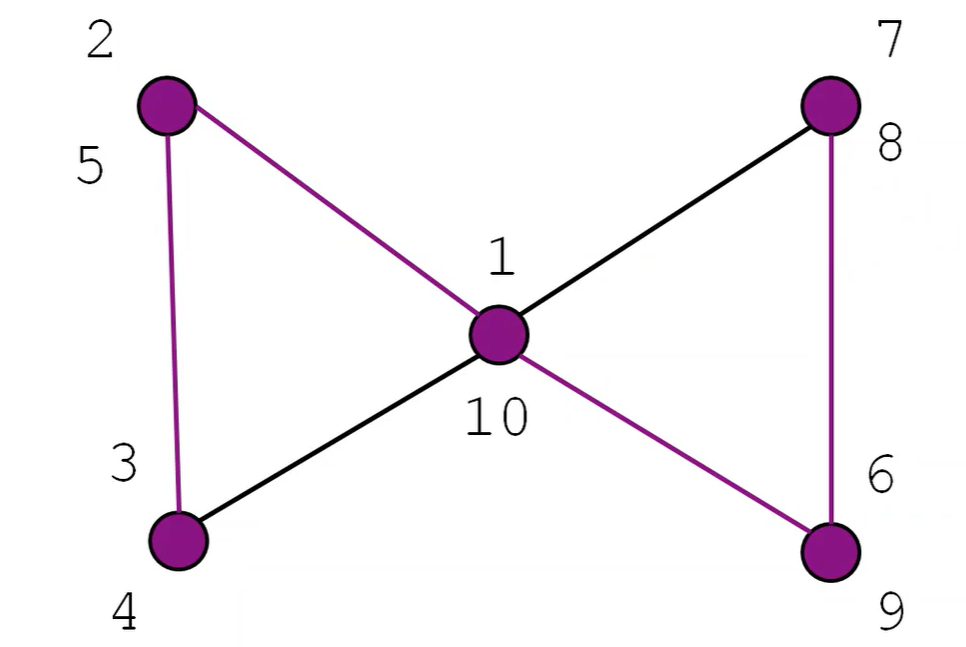
\includegraphics[scale=0.3]{assets/graph_tri_2.png}
\end{center}
How did we get this? 
\begin{itemize}
    \item We assign \code{1} to the center vertex. \code{1} has an unexplored neighbor, which is the top-left vertex.
    \item We assign \code{2} to the top-left vertex. \code{2} has an unexplored neighbor, which is the bottom-left vertex. 
    \item We assign \code{3} to the bottom-left vertex. \code{3} doesn't have any other unexplored neighbors.  
    \item Since we can't go anywhere from \code{3}, we assign it a post-order value of \code{4}.
    \item Now that we're back at \code{2}, note that there aren't any other unexplored edges, so we give it a post-order value of \code{5}.
    \item We're now back at the center vertex. However, we still have more to explore.
    \item We assign \code{6} to the bottom-right vertex. 
    \item We assign \code{7} to the top-right vertex. 
    \item Since we can't go anywhere from \code{7}, we assign it a post-order value of \code{8}.
    \item Now that we're back at \code{6}, we assign it a post-order value of \code{9} since we can't explore anything else.
    \item Now that we're back at \code{1}, we assign it a post-order value of \code{10} since we can't explore anything else. 
\end{itemize}
If the graph is connected, the first vertex will always be the last vertex. However, if the graph is disconnected, the first vertex may not necessarily be the last vertex. 

\subsubsection{Application of Orders}
\begin{proposition}
    For vertices $v$, $w$, we can consider the intervals \code{[v.pre, v.post]} and \code{[w.pre, w.post]}. These intervals:
    \begin{enumerate}
        \item contain each other if $v$ is an ancestor/descendant of $w$ in the DFS tree. 
        \item are disjoint if $v$ and $w$ are cousins in the DFS tree.
        \item never interleave (\code{v.pre < w.pre < v.post < w.post}).
    \end{enumerate}
\end{proposition}

\begin{mdframed}[]
    \begin{proof}
        Assume that the algorithm finds $v$ before $w$ (\code{v.pre < w.pre}). If the algorithm discovers $w$ after fully processing $v$, then: 
        \begin{itemize}
            \item \code{v.post < w.pre}
            \item Intervals are disjoint 
            \item $v$ and $w$ are cousins.
        \end{itemize}
        If the algorithm discovers $w$ before fully processing $v$:
        \begin{itemize}
            \item The algorithm finishes processing $w$ before it finishes $v$.
            \item \code{v.pre < w.pre < w.post < v.post}
            \item Represents nested intervals. 
            \item $v$ is an ancestor of $w$. 
        \end{itemize}
        And so we are done.
    \end{proof}
\end{mdframed}






































\newpage 
\section{Directed Graph Algorithms}
Often, an edge makes sense both ways. But, sometimes, streets are one directional.
\begin{definition}{}{}
    A \textbf{directed graph} is a graph where each edge has a direction. We say that it goes from $v$ to $w$. 
\end{definition}
Often, we draw arrows on the edges to denote direction. 

\bigskip 

A directed graph can be thought of as a graph of dependencies. For example, consider the following activities:
\begin{verbatim}
    Breakfast                       Go to work

                Wake up 

    Shower                          Dress 
\end{verbatim}
Of course, you can't do all five of these activities at the same time; there are some dependencies. Some of them are: 
\begin{itemize}
    \item Wake Up \textrightarrow{} Breakfast \textrightarrow{} Go to Work. 
    \item Wake Up \textrightarrow{} Go to Work. 
    \item Wake Up \textrightarrow{} Shower \textrightarrow{} Dress \textrightarrow{} Go to Work. 
\end{itemize}
In other words, you need to do $A$ before you can do $B$, and so on. One of the things we might want to do is order this graph in a way that respects these dependencies.

\subsection{Problem: DFS on Directed Graphs}
We can use DFS on a directed graph. However, we only follow directed edges from $v$ to $w$. The runtime is still $O(|V| + |E|)$, and \code{explore(v)} discovers all vertices reachable from $v$ following only directed edges. 


\subsection{Problem: Topological Ordering}
Essentially, a directed graph can be thought of as a graph of dependencies. An edge $v \mapsto w$ means that $v$ should come before $w$. We can use something known as topological ordering to better understand this relationship.

\begin{definition}{Topological Ordering}{}
    A \textbf{topological ordering} of a directed graph is an ordering of the vertices so that for each edge $(v, w)$, $v$ comes before $w$ in the ordering.
\end{definition}
\textbf{Remark:} There can be multiple different topological orderings for the same graph.

\bigskip 

\noindent
A question that we might have is: does every directed graph have a topological ordering?
\begin{itemize}
    \item No. Consider the classic counterexample:
    \[\text{Chicken } \mapsto \text{ Egg}\]
    \[\text{Egg } \mapsto \text{ Chicken}\]
    In other words, there is a \emph{cycle} where the chicken goes to the egg and the egg goes back to the chicken. 
\end{itemize}

\subsubsection{Cycles}
\begin{definition}{Cycle}{}
    A cycle in a directed graph is a sequence of vertices $v_1, v_2, \dots, v_n$ so that there are edges: 
    \[(v_1, v_2), (v_2, v_3), \dots, (v_n, v_1)\]
\end{definition}
For example, here is a cycle:
\begin{center}
    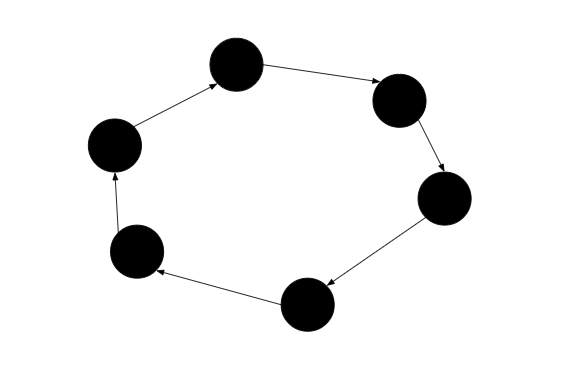
\includegraphics[scale=0.7]{assets/dir_graph_1.png}
\end{center}

\subsubsection{Obstacle}
\begin{proposition}
    If $G$ is a directed graph with a cycle, then $G$ has no topological ordering.
\end{proposition}
So, in other words, if $G$ is a directed graph with at least one cycle \emph{anywhere}, then it has no topological ordering.

\begin{mdframed}[]
    \begin{proof}
        Suppose we have a cycle $v_1, \dots, v_n$. Assume for the sake of contradiction taht we have an ordering. Then, there are $n$ vertices so one of them has to come first; say that $v_i$ came first in the ordering. But, this is a cycle so there is an edge from $v_{i - 1}$ to $v_i$. However, because $v_i$ was first so it must come first in the order, in contradiction to the order property. 
    \end{proof}
\end{mdframed}

\subsubsection{Directed Acyclic Graph (DAG)}
Suppose we want to focus on directed graphs with no cycles. This brings us to the following definition.
\begin{definition}{}{}
    A \textbf{directed acylic graph} (DAG) is a directed graph which contains no cycles. 
\end{definition}

The previous result said that only DAGs can be topologically ordered. However, is the reverse true? That is, is it the case that every DAG has a topological ordering? \textbf{Yes}. 

\subsubsection{Existence of Orderings}
\begin{theorem}{}{}
    Let $G$ be a (finite) DAG. Then, $G$ has a topological ordering.
\end{theorem}

\begin{mdframed}[]
    \begin{proof}
        We consider the last vertex in the ordering; in other words, whatever vertex comes last in this ordering. This vertex must be a sink, or a vertex with no outgoing edges. So, once we find the sink, we can put the graph at the end of the topological graph, and then order the remaining vertices. Now, using the lemma below, we want to show that every DAG has a topological ordering. We will use induction on $|G|$. Omitting the base case, we find a sink $v$. Then, create a graph $G' = G \setminus \{v\}$. We can inductively order $G'$, which is still a DAG. Then, add $v$ to the end of the ordering. 
    \end{proof}
\end{mdframed}

\subsubsection{Sinks}
\begin{lemma}{}{}
    Every finite DAG contains at least one sink. 
\end{lemma}

\begin{mdframed}[]
    \begin{proof}
        Start at a vertex $v = v_1$. Then, we can ``follow the trail,'' or in other words follow the edges $(v_1, v_2)$, $(v_2, v_3)$, \dots. Eventually, we will either find: 
        \begin{itemize}
            \item Some vertices repeat (which creates a cycle). This can't happen if this is a DAG, though. 
            \item Or, we get stuck (which means we found a sink).
        \end{itemize}
        So, we are done. 
    \end{proof}
\end{mdframed}

\subsubsection{Algorithm}
Suppose we want to design an algorithm that, given a DAG $G$, computes a topological ordering on G. We can use the proof to create a naive algorithm. 
\begin{itemize}
    \item Find a sink $v$. This is done by following a chain of vertices until we are stuck.
    \item Compute the ordering on $G - \{v\}$.
    \item Place $v$ at the end. 
\end{itemize}
This algorithm can be written like so: 
\begin{verbatim}
    TopologicalOrdering(G)
        If |G| = 0
            Return {}
        Let v in G 
        While there is an edge (v, w)
            v = w
        Return (Ordering(G - v), v)
\end{verbatim}
The runtime is $O(|V|^2)$. This is because we need $|V|$ time to find each sink and have $|V|$ sinks. This is suboptimal, however. Consider this optimal algorithm:
\begin{verbatim}
    TopologicalOrdering(G)
        Run DFS(G) w/ Pre/Post Numbers 
        Return Vertices in Reverse Postorder
\end{verbatim}
This runs in $O(|V| + |E|)$.

\subsubsection{Example: DAG}
Consider the following DAG which we will call $G$:
\begin{center}
    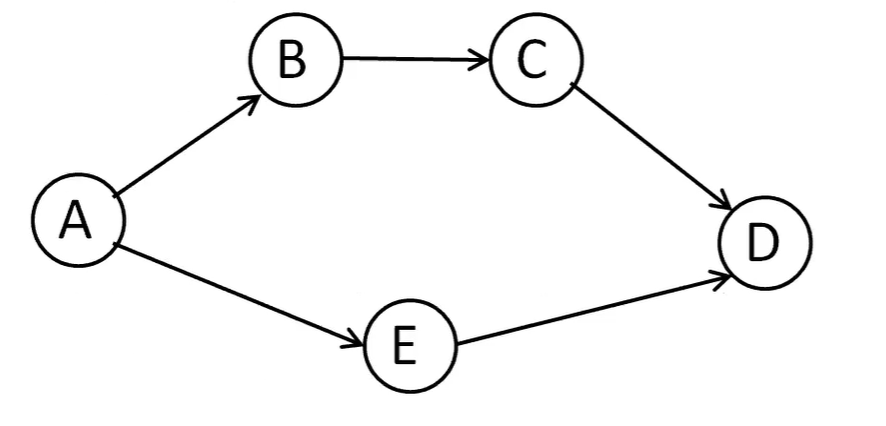
\includegraphics[scale=0.4]{assets/dag_ex.png}
\end{center}
We start at $A$ since this is where the graph ``begins.''
\begin{itemize}
    \item \underline{Using Algorithm 1:}
    \begin{itemize}
        \item First, we enumerate through the graph $G$ until we find a sink. In this case:
        \[A \mapsto B \mapsto C \mapsto D\]
        \item We \emph{remove} $D$ from the graph and add it to the ordering.
        \begin{verbatim}
            D
        \end{verbatim}
        \item Now, we enumerate through the graph $G - \{D\}$. In this case:
        \[A \mapsto B \mapsto C\]
        \item We \emph{remove} $C$ from the graph and add it to the ordering. 
        \begin{verbatim}
            C -> D
        \end{verbatim}
        \item Now, we enumerate through the graph $G - \{C, D\}$. In this case: 
        \[A \mapsto B\]
        \item We \emph{remove} $B$ from the graph and add it to the ordering. 
        \begin{verbatim}
            B -> C -> D
        \end{verbatim}
        \item Now, we enumerate through the graph $G - \{B, C, D\}$. In this case: 
        \[A \mapsto E\]
        \item We \emph{remove} $E$ from the graph and add it to the ordering. 
        \begin{verbatim}
            E -> B -> C -> D
        \end{verbatim}
        \item As we only have $A$ left, we can add it to the ordering. 
        \begin{verbatim}
            A -> E -> B -> C -> D
        \end{verbatim}
        So, we are done. 
    \end{itemize}

    \item \underline{Using Algorithm 2:}
    \begin{itemize}
        \item First, we enumerate through the graph $G$ until we find a sink. In this case: 
        \[A \mapsto B \mapsto C \mapsto D\]
        \item We remove $D$ from the graph and add it to the ordering. 
        \begin{verbatim}
            D
        \end{verbatim}
        \item Now, we remember that we already made it to $C$ and that $C$ is a sink in $G - \{D\}$. So, we remove $C$ and add it to the ordering: 
        \begin{verbatim}
            C -> D
        \end{verbatim}
        \item We remember that we already made it to $B$ and that $B$ is a sink in $G - \{C, D\}$. So, we remove $B$ and add it to the ordering: 
        \begin{verbatim}
            B -> C -> D
        \end{verbatim}
        \item Now that we're back at $A$, we note that $A$ has another edge. So, we go to that edge until we find a sink. In this case: 
        \[A \mapsto E\]
        \item We remove $E$ from the graph and add it to the ordering. 
        \begin{verbatim}
            E -> B -> C -> D
        \end{verbatim}
        \item Now, $A$ is the only vertex left in $G - \{B, C, D, E\}$. So, we add it to the ordering:
        \begin{verbatim}
            A -> E -> B -> C -> D
        \end{verbatim}
    \end{itemize}
    Here, we notice that algorithm 2 resembles depth-first seearch!
\end{itemize}

Another way to find a topological ordering for this graph is to consider the in-degrees of each vertex; i.e. the number of edges connecting \textbf{to} it. If we label each of $G$'s vertices with its in-degrees, we will have: 
\begin{center}
    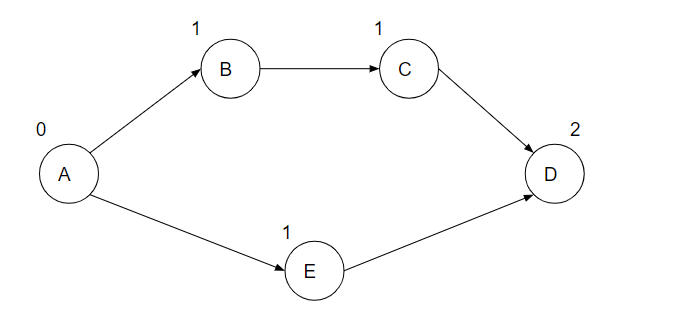
\includegraphics[scale=0.7]{assets/dag_ex_deg_1.png}
\end{center}
So, this makeshift algorithm is essentially:
\begin{verbatim}
    TopologicalOrdering(G)
        ordering = []
        while G is not empty
            v = vertex in G with lowest in-degree (i.e. in-degree 0)
            ordering.append(v)
            Remove v from G
            Update in-degrees of existing vertices
        return ordering  
\end{verbatim}
\begin{itemize}
    \item First, note that $A$ has the lowest in-degree. So, remove $A$ from the graph and add it to the ordering. The ordering now looks like: 
    \begin{verbatim}
        [A]
    \end{verbatim}
    \item The graph now looks like: 
    \begin{center}
        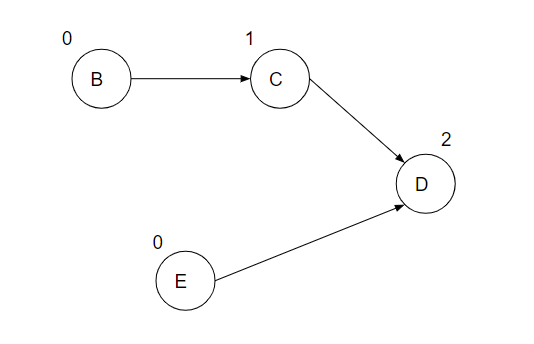
\includegraphics[scale=0.4]{assets/dag_ex_deg_2.png}
    \end{center}
    Here, $B$ and $E$ both have the lowest in-degree. So, we can remove one or the other. For the sake of consistency, remove $E$ from the graph and add it to the ordering. The ordering now looks like: 
    \begin{verbatim}
        [A, E]
    \end{verbatim}
    \item The graph now looks like:
    \begin{center}
        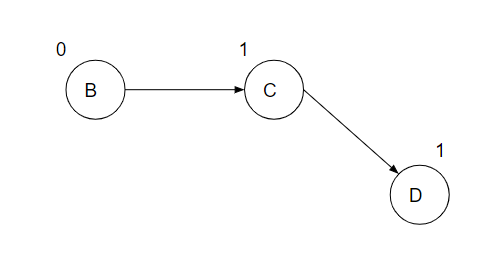
\includegraphics[scale=0.4]{assets/dag_ex_deg_3.png}
    \end{center}
    Here, note that $B$ is the only node with the lowest in-degree. So, we remove it and add it to the ordering. The ordering now looks like: 
    \begin{verbatim}
        [A, E, B]
    \end{verbatim}
    \item The graph now looks like:
    \begin{center}
        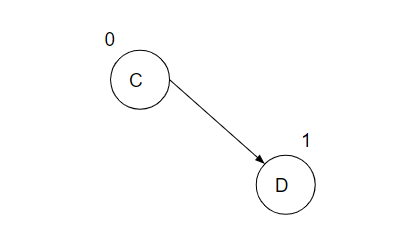
\includegraphics[scale=0.4]{assets/dag_ex_deg_4.png}
    \end{center}
    Here, $C$ has the lowest in-degree so we remove it and add it to the ordering. The ordering now looks like: 
    \begin{verbatim}
        [A, E, B, C]
    \end{verbatim}
    \item By now, it's trivial to see that $D$ has in-degree 0, so we add it.
    \begin{verbatim}
        [A, E, B, C, D]
    \end{verbatim}
    And we are done. 
\end{itemize}

\subsubsection{Topological Sort}
This is a particularly useful algorithm. 
\begin{itemize}
    \item Many graph algorithms are relatively easy to find the answer for $v$ if you've already found the answer for everything downstream of $v$. 
    \begin{itemize}
        \item We can topologically sort $G$. 
        \item Then, solve for $v$ in reverse topological order.
    \end{itemize}
\end{itemize}


\subsection{Problem: Strongly Connected Components \& Metagraphs}
In undirected graphs, we had a very clean description of reachability: $v$ was reachable from $w$ if and only if they were in the same connected component. Well, this no longer works for digraphs. How do we achieve a clean description of reachability in a directed graph? 
\begin{itemize}
    \item Note that reachability is no longer symmetric. That is, we can reach $w$ from $v$ but not the other way around. 
    \item Can we maybe allow reachability in either direction?
    \item Maybe we can allow the ability to follow edges in either direction? However, this treats a digraph as an undirected graph. 
\end{itemize}

\begin{definition}{Strongly Connected Components}{}
    In a directed graph $G$, two vertices $v$ and $w$ are in the same \textbf{strongly connected component} if $v$ is reachable from $w$ and $w$ is reachable from $v$.
\end{definition}

\subsubsection{Equivalence Relation}
Let $v \sim w$ if $v$ is reachable from $w$ and vice versa.
\begin{proposition}
    This is an equivalence relation. Namely:
    \begin{itemize}
        \item $v \sim v$ ($v$ is reachable from itself).
        \item $v \sim w \implies w \sim v$ (relation is symmetric).
        \item $u \sim v \text{ and } v \sim w \implies u \sim w$.
    \end{itemize}
\end{proposition}

\subsubsection{Relationship to Components}
Essentially, when we have this equivalence relation, we can split a set into components (equivalence classes) so that $v \sim w$ if and only if $v$ and $w$ are in the same component.

\bigskip 

Take any $v$, the set of all $w$ so that $v \sim w$ is the component of $v$. Then, everything connects to everything else in this equivalence class and does not connect (both ways) to anything outside. 

\subsubsection{Example: SCCs}
Consider the following graph:
\begin{center}
    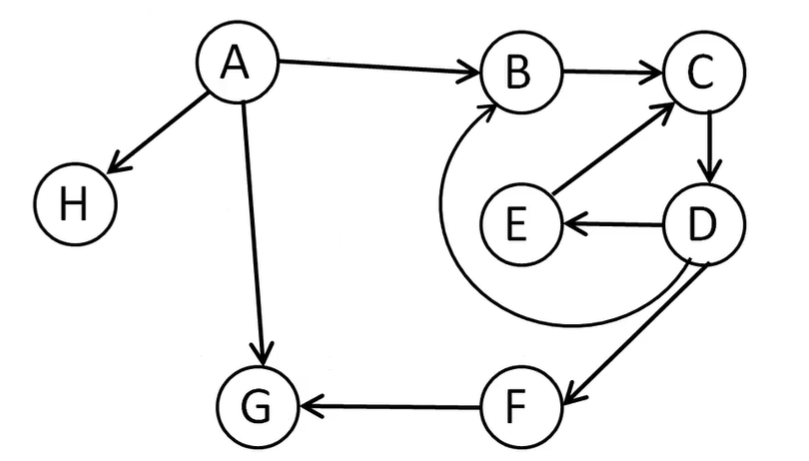
\includegraphics[scale=0.4]{assets/scc.png}
\end{center}
How many strongly connected components does this graph have? 

\begin{mdframed}[]
    The answer is \textbf{5}. If we use the idea of equivalence classes above, then the equivalence classes are: 
    \begin{itemize}
        \item $B$, $C$, $D$, $E$. 
        \item $A$
        \item $H$
        \item $G$
        \item $F$
    \end{itemize}
    Here, we note that $B$, $C$, $D$, and $E$ are all reachable from each other. However, these vertices and, for example, $A$ are not reachable both ways. 
\end{mdframed}

\subsubsection{Connectivity}
Do strongly connected components completely describe connectivity in $G$?
\begin{itemize}
    \item \textbf{No}. In directed cases, we can have an edge between strongly connected components. In the undirected case, connected components told you everything that there was to know. However, in the directed case, we can have these two strongly connected components consisting of just a single vertex $v$ and $w$. However, just knowing these components doesn't tell you if there is an edge from $v$ to $w$ or vice versa. There could be an edge that could be extra information that we need to know. 
    \begin{verbatim}
        [v] ---------> [w]
    \end{verbatim}

    \item We need extra information to describe how SCCs connect. 
\end{itemize}

\subsubsection{Metagraph}
\begin{definition}{Metagraph}{}
    The \textbf{metagraph} of a directed graph $G$ is a graph whose vertices are the strongly connected components of $G$, where there is an edge between $C_1$ and $C_2$ if and only if $G$ has an edge between some vertex of $C_1$ and some vertex of $C_2$. 
\end{definition}
\textbf{Remark:} If you're given the strongly connected components and the metagraph of a graph $G$, then you can you can figure out connectivity within the full graph.

\bigskip

So, the corresponding metagraph of the above graph in the example would be: 
\begin{center}
    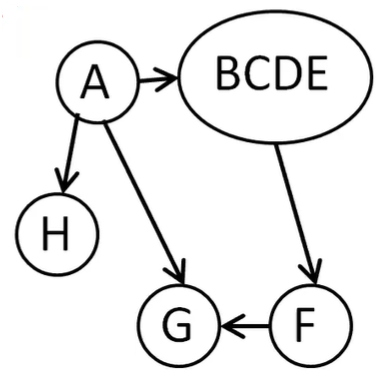
\includegraphics[scale=0.6]{assets/scc_meta.png}
\end{center}

\subsubsection{Result}
\begin{theorem}{}{}
    The metagraph of any directed graph is a DAG. 
\end{theorem}

\begin{mdframed}[]
    \begin{proof}
        Assume for the sake of contradiction that it is not a DAG. Then, the metagraph has a cycle. Now, let's suppose we have a bunch of strongly connected components; call these SCCs $C_1, C_2, \dots, C_n$. Then, since the metagraph has a cycle, then the strongly connected components form a cycle. That is, we can go from $C_1$ to $C_2$ to $C_n$ back to $C_1$. However, this implies that we have one giant strongly connected component since we can get from one $C_i$ to another $C_j$ ($i \neq j$) and vice versa.     
    \end{proof}
\end{mdframed}

\subsubsection{Easy Algorithm to Compute SCC \& Metagraph}
Given a directed graph $G$, compute the SCCs of $G$ and its metagraph. 
\begin{itemize}
    \item For each $v$, compute vertices reachable from $v$.
    \item Find pairs $v$, $w$ so that $v$ reachable from $w$ and vice versa.
    \item For each $v$, the corresponding $w$'s are in the SCC of $v$.
\end{itemize}
The runtime is $O(|V|(|V| + |E|))$.

\subsubsection{Observation and Better Algorithm}
Suppose that $SCC(v)$ is a sink in the metagraph.
\begin{itemize}
    \item $G$ has no edges from $SCC(v)$ to another $SCC$. 
    \item We can run \code{explore(v)} to find all vertices reachable from $v$. This will contain all vertices in $SCC(v)$. But, it contains no other vertices. 
    \item If $v$ is in the SCC, then \code{explore(v)} finds exactly $v$'s component. 
\end{itemize}
With this observation, we consider the following strategy:
\begin{itemize}
    \item Find $v$ in a sink SCC of $G$. 
    \item Run \code{explore(v)} to find the component $C_1$.
    \item Repeat process on $G \setminus C_1$.
\end{itemize}
The problem is, how do we find $v$ that is in a sink?
\begin{proposition}
    Let $C_1$ and $C_2$ be SCCs of $G$ with an edge from $C_1$ to $C_2$. If we run \code{DFS} on $G$, the largest postorder number of any vertex in $C_1$ will be larger than the largest postorder number in $C_2$. 
\end{proposition}

The reason why we care is because if $v$ is the vertex with the largest postorder number, then: 
\begin{itemize}
    \item There is no edge to $SCC(V)$ from any other SCC. 
    \item SCC is a \underline{source} SCC.
\end{itemize}
However, we wanted a \emph{sink} SCC. So, how do we relate these two?
\begin{itemize}
    \item A sink is like a source, only with edges going in the opposite direction.
\end{itemize}
So, we define a reverse graph like so: 
\begin{definition}{Reverse Graph}{}
    Given a directed graph $G$, the \textbf{reverse graph} of $G$ (denoted $G^R$) is obtained by reversing the directions of all the edges of $G$.
\end{definition}
Some properties of reverse graphs are: 
\begin{itemize}
    \item $G$ and $G^R$ have the same number of vertices and edges. 
    \item $G = (G^R)^R$. 
    \item $G$ and $G^R$ have the same SCCs. 
    \item The sink SCCs of $G$ are the source SCCs of $G^R$. 
    \item The source SCCs of $G$ are the sink SCCs of $G^R$. 
\end{itemize}

The better algorithm we have is: 
\begin{verbatim}
    SCCs(G)
        Run DFS(G^R), record postorder 
        Find v with largest v.post 
        Set all vertices unvisited 
        Run explore(v)
        Let C be the visited vertices 
        Return SCCs(G - C) union {C}
\end{verbatim}

The issue with our algorithm is that we recompute the postorder for every SCC we need to find. However, we don't need to do this; rather, after removing some strongly connected components to get $G'$, the largest postorder number of vertices in $G'$ is still in a sink component of $G'$. 

\subsection{Better Algorithm}
\begin{verbatim}
    SCCs(G)
        Run DFS(G^R), record postorders
        Mark all vertices as unvisited 
        For v in V in reverse postorder 
            If v not in a component yet     // if v is not visited 
                explore(v) on G-components found,
                marking new component 
\end{verbatim}

So, really, this is just 2 DFSs, so the runtime is $O(|V| + |E|)$. 

















\newpage 
\section{Paths in Graphs}
DFS and \code{explore} allow us to determine \emph{if} it is possible to get from one vertex to another, and using the DFS tree, you can also find a path. However, this is often not an efficient path. This is because DFS picks one path and tries to go to the end of that path before trying a different path. If that path happens to be a not-so-ideal path, then we've taken a much longer path than necessary. For example, consider the following graph:
\begin{center}
    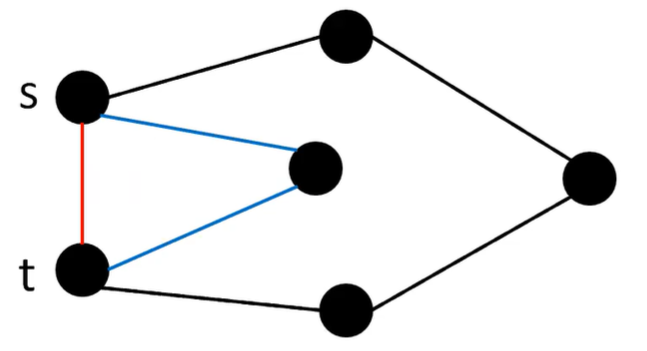
\includegraphics[scale=0.4]{assets/dfs_bfs_comp.png}
\end{center}
Suppose we wanted to get from $s$ to $t$. Using DFS, we might take the black path; the one with 4 edges. How do we guarantee that we take the shortest path, i.e. the red path? 

\subsection{Problem: Finding Shortest Path in Unweighted Graph}
Given a graph $G$ with two vertices $s$ and $t$ in the same connected component, how do we find the \emph{best} path from $s$ to $t$? In fact, what do we mean by the best path? 
\begin{itemize}
    \item Least expensive. 
    \item Best scenery.
    \item Shortest.
\end{itemize}
For now, we want the fewest edges. 

\subsubsection{Observation}
\begin{proposition}
    If there is a path from vertices $s$ to $v$ with length at most $d$, then there is some $w$ adjacent to $v$ where there is a path a length at most $(d - 1)$ from vertices $s$ to $w$.
\end{proposition} 

\begin{mdframed}[]
    \begin{proof}
        If $w$ is the next-to-last vertex on the path, then there are $d$ edges to get you from $s$ to $v$ and that means the number of edges you have to take from $s$ to $w$ is only $d - 1$. This means that if we know all of the vertices with distance at most $d - 1$, then we can find all of the vertices with distance at most $d$.
    \end{proof}
\end{mdframed}

For example, consider the following (annotated) graph:
\begin{center}
    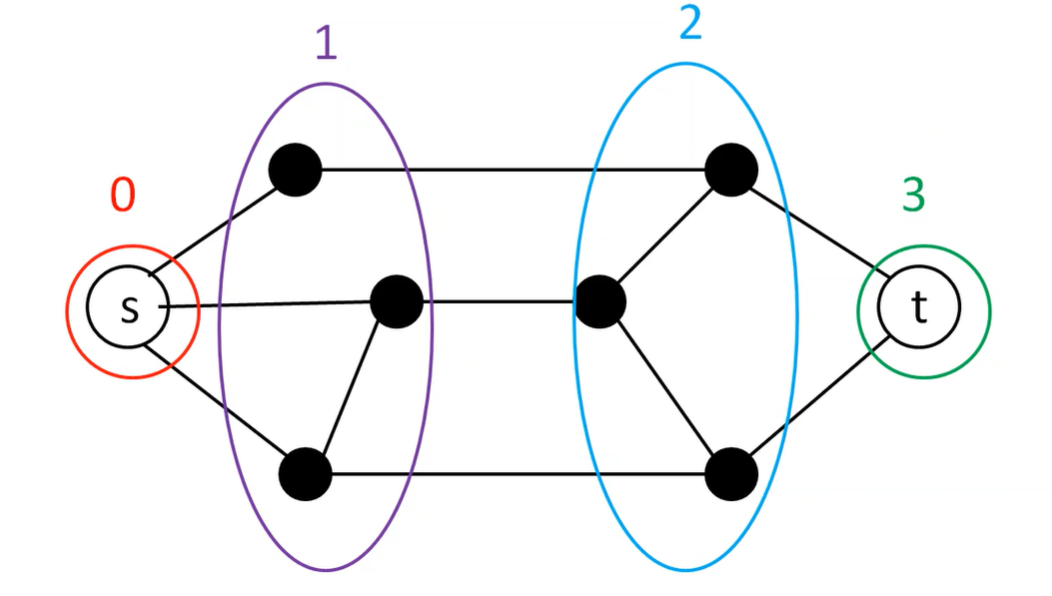
\includegraphics[scale=0.4]{assets/1_2_3_dist.png}
\end{center}
Here, suppose we start at $s$.
\begin{itemize}
    \item The only place we can get with a path of length 0 is $s$, or the one vertex in the red circle labeled \code{0}.
    \item If we want to travel one edge, the only places we can get with a path of length one are the vertices in the purple circle labeled \code{1}.
    \item If we want to travel two edges, we can get to some vertex that is adjacent to one of the vertices in the purple circle. For each of the purple vertices, if we list all of the adjacent vertices, the only new vertices we can reach are the vertices in the cyan circle labeled \code{2}.
    \item Finally, if we want to travel three edges, we can get to something that is adjacent to the vertices at distance 2, which means we can get to $t$, or the vertex in the green circle labeled \code{3}. 
\end{itemize}
By the way we constructed these sets (the circles), it's not possible to get to $t$ at distance 2 because, for that to happen, it has to be adjacent to the vertices at distance 1, which it isn't.

\subsubsection{Algorithm Idea}
This observation gives us a pretty reasonable way to find an algorithm. In particular, if we want to find the best path length between $s$ and $t$, we really need to find the best path length between $s$ and every other vertex in the graph.

\bigskip 

So, the idea is, for each $d$, create a list of all vertices at distance $d$ from $s$.
\begin{itemize}
    \item For $d = 0$, this is just $\{s\}$.
    \item For larger $d$, we want all new vertices adjacent to vertices at distance $d - 1$.
\end{itemize}

\subsubsection{Algorithm}
The algorithm is as follows:
\begin{verbatim}
    1    ShortestPaths(G, s)
    2        Initialize Array A
    3        A[0] = {s}
    4        dist(s) = 0
    5        For d = 0 to n
    6            For u in A[d]
    7                For (u, v) in E
    8                    if dist(v) undefined
    9                        dist(v) = d + 1
    10                       add v to A[d + 1]
\end{verbatim}

\subsubsection{Improving the Algorithm}
How can we improve this?
\begin{itemize}
    \item What if \code{dist(v)} undefined at end? We can set the distances of all vertices to infinity.\footnote{Note that \code{+} next to a line number means added code and \code{c} next to a line number means changed line.}
    \begin{verbatim}
        1    ShortestPaths(G, s)
        2+       For each v in V, dist(v) = infinity 
        3        Initialize Array A
        4        A[0] = {s}
        5        dist(s) = 0
        6        For d = 0 to n
        7            For u in A[d]
        8                For (u, v) in E
        9c                   if dist(v) = infinity
        10                       dist(v) = d + 1
        11                       add v to A[d + 1]
    \end{verbatim}
    Here, at the end of the algorithm, any vertices that could not be found will be assigned a distance of infinity to indicate that it could not be reached. 

    \item The algorithm goes through \code{A[0]}, \code{A[1]}, and so on in order. We can just use a queue.
    \begin{verbatim}
        1    ShortestPaths(G, s)
        2        For each v in V, dist(v) = infinity 
        3c       Initialize Queue Q
        5        dist(s) = 0
        6c       While Q not empty
        7c           u = front(Q)
        8            For (u, v) in E
        9                if dist(v) = infinity
        10c                  dist(v) = dist(u) + 1
        11c                  Q.enqueue(v)
    \end{verbatim}

    \item What if we want to keep track of the paths? 
    \begin{verbatim}
        1    ShortestPaths(G, s)
        2        For each v in V, dist(v) = infinity 
        3        Initialize Queue Q
        4        dist(s) = 0
        5        While Q not empty
        6            u = front(Q)
        7            For (u, v) in E
        8                if dist(v) = infinity
        9                    dist(v) = dist(u) + 1
        10                   Q.enqueue(v)
        11+                  v.prev = u     // Keep track of path
    \end{verbatim}
    With this change, we can simply follow the chain of \code{prev}ious vertices, which is the path that was taken. 
\end{itemize}

\subsubsection{Breadth First Search}
In our last change above, we note that we simply have BFS.
\begin{verbatim}
    BFS(G, s)
        For v in V, dist(v) = infinity 
        Initialize Queue Q
        Q.enqueue(s)
        dist(s) = 0
        While Q is not empty
            u = front(Q)
            For (u, v) in E
                If dist(v) = infinity
                    dist(v) = dist(u) + 1
                    Q.enqueue(v)
                    v.prev = u
\end{verbatim}
The total runtime is $O(|V| + |E|)$.
\begin{itemize}
    \item In the first few lines, we have $O(|V|)$ time.
    \item In the while loop and the \code{front(Q)} lines, we have $O(|V|)$ iterations. 
    \item In the edge iteration, we have $O(|E|)$ iterations. 
\end{itemize}

\subsubsection{DFS vs. BFS}
\begin{itemize}
    \item Similarities:
    \begin{itemize}
        \item The way both algorithms process vertices is the same (\code{visited} for DFS vs. \code{dist < infinity} for BFS).
        \item For each vertex, process all unprocessed neighbors.
    \end{itemize}
    \item Differences:
    \begin{itemize}
        \item DFS uses a stack to store vertices waiting to be processed. 
        \item BFS uses a queue.
    \end{itemize}
    \item Big Effect:
    \begin{itemize}
        \item DFS goes depth-first: very long path. Get a very ``skinny'' tree. 
        \item BFS is breadth first: visits all side paths. Get a very shallow tree since we process all of the neighbors.
    \end{itemize}
\end{itemize}

\subsubsection{Edge Length}
The number of edges in a path is not always the right measure of distance. Sometimes, taking several shorter steps is preferably to taking a few longer ones. 

\bigskip 

We can assign each edge $(u, v)$ a non-negative \underline{length} $\ell(u, v)$. The length of a path is the sum of the lengths of its edges.






\subsection{Problem: Finding Shortest Path in Weighted Graph}
Given a graph where each edge has some length $\ell$, how do we find the shortest path between two vertices? 


\subsubsection{Trivial Way}
The idea is the break edges into unit length edges. So, an edge of length 5 can actually be seen as 5 edges of length 1. With this conversion, we can run BFS. 
\begin{center}
    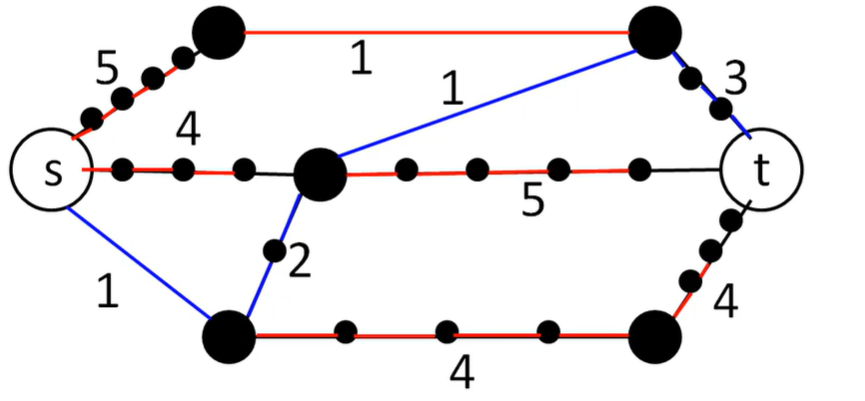
\includegraphics[scale=0.4]{assets/bfs_unit_edges.png}
\end{center}
Here, we see that the blue path has distance 7 (the lowest) while the red paths are the other paths that the BFS algorithm took. 

\bigskip 

Now, this \emph{works}. However, there are some issues. 
\begin{itemize}
    \item BFS is linear time for the graph that we run it on. However, we're breaking this graph up so every edge can be represented as a unit edge (so an edge of weight $n$ becomes $n$ edges of weight 1). The runtime is $\BigO(\text{Sum of Edge Lengths})$.
    \item What if we have an edge of length one million? 
    \item What if our edges have decimal weights (e.g. $\pi$, $15.12314352452$, so on)?
\end{itemize}

\subsubsection{Another Way}
If we have very long edge lengths, most steps will just consist of advancing slightly (one unit) along a bunch of edges. The issue is, there may be a time period where all we're doing is advancing along one unit for each path that BFS is taking. 

\bigskip 

So, how do we ``fast forward'' through these boring steps? Well, occasionally, we have an interesting step where, for instance, the wavefront hits a new vertex. In other words, every time you hit a new vertex, you might need to update some things. But, ignoring that, all we're really doing is slowly advancing through each edge. 

\subsubsection{Algorithm}
This algorithm is associated with the ``ooze'' that was mentioned in lecture. 
\begin{verbatim}
    Distances(G, s, l)
        dist(v) = 0
        While not all distances found 
            Find minimum over (v, w) in E
                with v discovered w not 
                of dist(v) + l(v, w)
            dist(w) = dist(v) + l(v, w)
            prev(w) = v
\end{verbatim}

\subsubsection{Why Does This Work?}
\begin{proposition}
    Whenever the algorithm assigns a distance to a vertex $v$, that is the length of the shortest path from $s$ to $v$. 
\end{proposition}

\begin{mdframed}[]
    \begin{proof}
        We use induction.
        \begin{description}
            \item[Base Case:] We know that \code{dist(s) = 0}. The empty path has length 0. 
            \item[Inductive Step:] When assigning distances to $w$, suppose that all previously assigned distances are correct. We can imagine a bubble containing the vertices $s$ and $v$, with edge denoted by $\text{dist}(v)$. By the inductive hypothesis, we assume that all edge lengths inside this bubble is correct. Take a vertex $w$ which is outside of the bubble so that the path length from $v$ (inside the bubble) to $w$ has length $\ell(v, w)$. This is the shortest path from $s$ to any vertex outside the bubble. 
        \end{description}
    \end{proof}
\end{mdframed}

\subsubsection{Runtime of Initial Algorithm}
This runs in $\BigO(|V| \cdot |E|)$ time. There are $\BigO(|V|)$ iterations and $\BigO(|E|)$ edges.
\begin{itemize}
    \item This is too slow because every iteration we have to check every edge. 
    \item The idea is that most of the comparison doesn't change much iteration to iteration. So, we can use this to save time. 
    \item Specifically, record for each $w$ the best value of $\text{dist}(v) + \ell(v, w)$. 
\end{itemize}

\subsubsection{Better Algorithm}
Our better algorithm is based on the observations that we had above.
\begin{verbatim}
    Distances(G, s, l)
        For v in V 
            dist(v) = infinity 
            done(v) = false 
        dist(s) = 0
        done(s) = false 

        while not all vertices done 
            Find v not done with minimum dist(v)
            done(v) = true 
            For (v, w) in E 
                if dist(v) + l(v, w) < dist(w)
                    dist(w) = dist(v) + l(v, w)
                    prev(w) = v
\end{verbatim}
The initialization is $O(|V|)$, and the while loop is $\BigO(|V|)$. The for loop is $\BigO(|E|)$ time. Thus, the runtime is: 
\[\BigO(|V|^2 + |E|)\]
\begin{itemize}
    \item This repeatedly asks for the smallest vertex. Even though not much is changing from round to round, the algorithm is computing the minimum from scratch every time.
    \item We can use a data structure to help answer a bunch of similar questions faster than answering each question individually (like the one above).
\end{itemize}

\subsubsection{Priority Queue}
A \textbf{priority queue} is a data structure that stores elements sorted by a \textbf{key} value. Its operations are: 
\begin{itemize}
    \item \code{insert}: Adds a new element to the priority queue.
    \item \code{decreaseKey}: Changes the key of an element of the priority queue to a specified smaller value. 
    \item \code{deleteMin}: Deletes the element with the lowest key from the priority queue. 
\end{itemize}

\subsubsection{Even Better Priority Queue}
\begin{verbatim}
    Dijkstra(G, s, l)
        Initialize Priority Queue Q 
        For v in V
            dist(v) = infinity
            Q.insert(v) // using dist(v) as key
        dist(s) = 0
        while Q not empty
            v = Q.deleteMin()
            For (v, w) in E
                if dist(v) + l(v, w) < dist(w)
                    dist(w) = dist(v) + l(v, w)
                    prev(w) = v
                    // w has a faster path and needs to updated in
                    // the priority queue 
                    Q.decreaseKey(w)
\end{verbatim}
The runtime is as follows: 
\begin{itemize}
    \item We need to iterate $\BigO(|V|)$ times for the initial loop. 
    \item In the \code{while} loop, we run $\BigO(|V|)$ times. 
    \item We need to run through the edges $\BigO(|E|)$ times. 
\end{itemize}
So, $\BigO(|V|)$ \code{insert}s + $\BigO(|V|)$ \code{deleteMin}s + $\BigO(|E|)$ \code{decreaseKey}. The runtime of Dijkstra's algorithm now depends on what priority queue we use. 

\subsubsection{Priority Queue Implementations}
Here, we go over some implementations of priority queues. 

\begin{itemize}
    \item \textbf{Unsorted List:} Store $n$ elements in an unsorted list. 

    \begin{center}
        \begin{tabular}{p{0.85in}|p{0.75in}|p{4in}}
            \textbf{Operation} & \textbf{Runtime} & \textbf{Explanation} \\ 
            \hline 
            \code{Insert}      & $\BigO(1)$ & Add it at the end of the list. \\ 
            \code{DecreaseKey} & $\BigO(1)$ & Assuming the operation comes with a pointer to where the element is stored in your data structure, take that element and decrease its key value. \\ 
            \code{DecreaseMin} & $\BigO(n)$ & We need to potentially scan the entire list. \\ 
        \end{tabular}
    \end{center}
    For Dijkstra, we would have $\BigO(|V|^2 + |E|)$. 


    \item \textbf{Binary Heap:} Store elements in a balanced binary tree with each element having smaller key value than its children.

    \begin{center}
        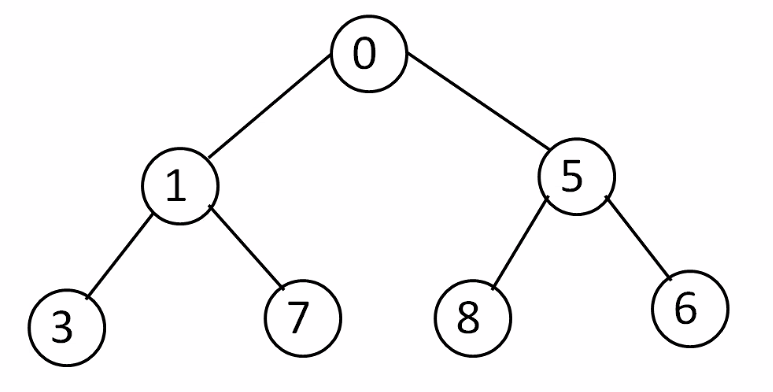
\includegraphics[scale=0.5]{assets/bin_heap.png}
    
        \textbf{Figure:} A binary heap.
    \end{center}
    The smallest key is at the top (\code{0}) and there are $\log{n}$ levels. 
    
    \begin{center}
        \begin{tabular}{p{0.85in}|p{0.75in}|p{4in}}
            \textbf{Operation} & \textbf{Runtime} & \textbf{Explanation} \\ 
            \hline 
            \code{Insert}      & $\BigO(\log(n))$ & Add the key at the bottom, then bubble the new key up until it's in the right place. \\ 
            \code{DecreaseKey} & $\BigO(\log(n))$ & We need to change the key. Then, we might need to bubble up the changed key until it's in the right place. \\ 
            \code{DecreaseMin} & $\BigO(\log(n))$ & We remove and then return the root node. Then, we move the bottom-most node to the root. After this, we might need to continuously bubble down the root node until it's in the right place. \\ 
        \end{tabular}
    \end{center}
    For Dijkstra, we would have $\BigO(\log(|V|)(|V| + |E|))$. 

    \item \textbf{d-ary Heap:} This is like a binary heap, but each node has $d$ children. 
    
    \begin{center}
        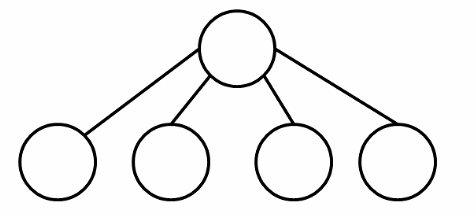
\includegraphics[scale=0.5]{assets/dary_heap.png}
    
        \textbf{Figure:} A 4-ary heap.
    \end{center}
    
    There are $\frac{\log(n)}{\log(d)}$ levels, so bubble up is faster. However, bubble down is slower since we need to compare more children. 
    
    \begin{center}
        \begin{tabular}{p{0.85in}|p{0.75in}|p{4in}}
            \textbf{Operation} & \textbf{Runtime} & \textbf{Explanation} \\ 
            \hline 
            \code{Insert}      & $\BigO\left(\frac{\log(n)}{\log(d)}\right)$ & Same thing as binary heap, essentially. \\ 
            \code{DecreaseKey} & $\BigO\left(\frac{\log(n)}{\log(d)}\right)$ & Same idea as binary heap, \emph{but} the bubbling up is a lot faster. \\ 
            \code{DecreaseMin} & $\BigO\left(\frac{d\log(n)}{\log(d)}\right)$ & This is because, for bubble down, we need to compare more children; specifically, the $d$ children. \\ 
        \end{tabular}
    \end{center}
    For Dijkstra, we would have $\BigO\left(\frac{\log(|V|)(d|V| +|E|)}{\log(d)}\right)$. If the number of edges is substantially greater than the number of vertices, this can potentially be an improvement. 

    
    \item \textbf{Fibonacci Heap:} This is an advanced data structure that uses amortization\footnote{So, you might spend more time on a particular operation, but the overall runtime will be ``consistent.''}. We are not concerned with its implementation. 

    \begin{center}
        \begin{tabular}{p{0.85in}|p{0.75in}}
            \textbf{Operation} & \textbf{Runtime} \\ 
            \hline 
            \code{Insert}      & $\BigO(1)$ \\ 
            \code{DecreaseKey} & $\BigO(1)$ \\ 
            \code{DecreaseMin} & $\BigO(\log(n))$ \\ 
        \end{tabular}
    \end{center}
    For Dijkstra, we would have $\BigO(|V|\log(|V|) + |E|)$. This is the most ideal runtime, and thus the runtime that we can assume. 
\end{itemize}
Therefore, with a Fibonacci Heap, Dijkstra's algorithm would have a runtime of $\boxed{\BigO(|V|\log(|V|) + |E|)}$.



\subsection{Problem: Finding Shortest Path in Unweighted Graph with Negative Edge Weights}
So far, we've talked about non-negative lengths. However, depending on what we're representing as lengths, we might have \emph{negative} lengths. That being said, the problem statement is the same - find the path with the smallest sum of edge weight. 

\bigskip 

Right now, Dijkstra's algorithm doesn't actually work on negative edge values. To see why this is the case, consider the following visualization: 
\begin{center}
    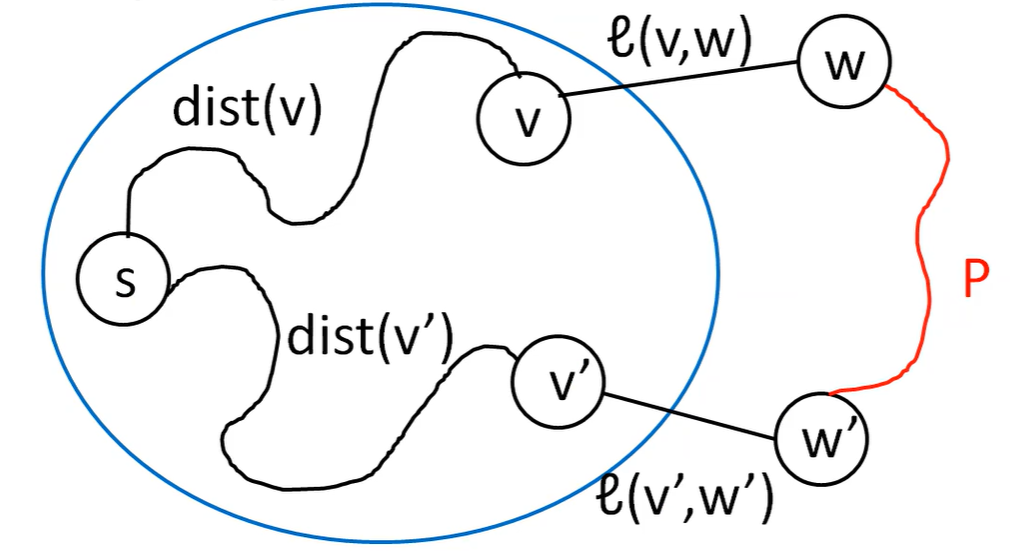
\includegraphics[scale=0.3]{assets/neg_bubble.png}
\end{center}
Here, the bubble represents all correctly assigned distances. In other words, here, $s$ and and $v$ has edge length $\text{dist}(v)$, the shortest distance between the two. Then, from $v$ (inside the bubble) to $w$ (outside the bubble), if we consider the edge length $\ell(v, w)$, it follows that this must be the shortest path. The point was that this must be the right distance to $w$; any other way to get to $w$ means that we would have to leave the bubble some other way (in our case, from $s$ to $v'$ to $w'$). Then, there has to be a path connecting $w'$ to $w$, of which we denote $P$. So, it follows that:  
\[\text{dist}(v) + \ell(v, w) \leq \text{dist}(v') + \ell(v', w') + \ell(P)\]
This correctly works if $\ell(P)$ is non-negative. However, if $\ell(P)$ is negative, we run into an issue. 

\bigskip 

Thus, the problem becomes: find the shortest path from one vertex to another when there are potnetially negative edge weights. 

\subsubsection{Negative Weight Cycles}
\begin{definition}{}{}
    A \textbf{negative weight cycle} is a cycle where the total weight of edges is negative. 
\end{definition}
\textbf{Remarks:}
\begin{itemize}
    \item If $G$ has a negative weight cycle, then there are probably no shortest paths since we can go around the cycle over and over again. 
    \item For an undirected graph $G$, a single negative weight edge gives a negative weight cycle by going back and forth on it. So, we usually don't talk about the negative edge weight in the context of an undirected graph. 
\end{itemize}
For example, consider the following graph:
\begin{center}
    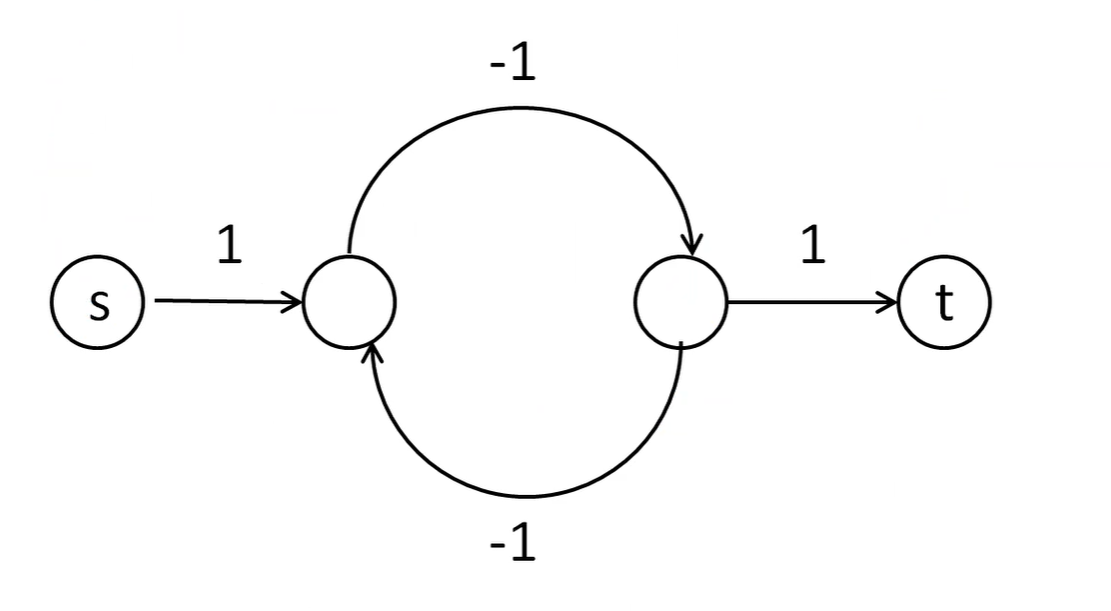
\includegraphics[scale=0.2]{assets/neg_cycle_1.png}
\end{center}
Here, the shortest path length from $s$ to $t$ is as small as we like it to be. So, really, the shortest path length is $-\infty$. This graph\textbf{also} answers an important question:
\begin{mdframed}[]
    What stops us from adding a constant to every edge length so every edge length is non-negative, thus letting us run Dijkstra's algorithm? 
\end{mdframed}
Well, if we added a constant to every edge length so that every edge length is non-negative, then there would only be one answer. For example, if we added 1 to each edge length, the shortest path becomes $2 + 0 + 2 = 4$. But since we added 1 to each edge length and we went through three edges, our final answer is $1$. \emph{However}, this completely avoids the fact that we could just loop around the negative cycle many times. 

\subsubsection{Fundamental Shortest Paths Formula}
For any vertex $w$ that isn't the source $s$, $w \neq s$,
\[\text{dist}(w) = \min_{(v, w) \in E} \text{dist}(v) + \ell(v, w)\]
This says that the distance of $w$ is equal to the minimum over all edges $v$ to $w$ in $E$ of the distance to $v$ plus the length of the edge from $v$ to $w$. 
\begin{center}
    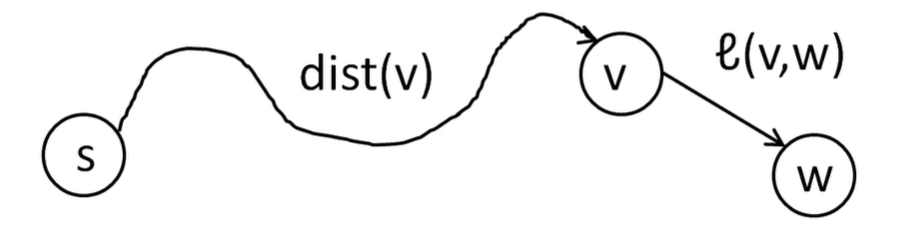
\includegraphics[scale=0.4]{assets/fun_sho_path.png}
\end{center}
Looking at the visualization above, we're saying that the path from $s$ to $v$ has length $\text{dist}(v)$; this is the shortest path from $s$ to $v$.

\bigskip 

We can use a system of equations to solve for the distances from $s$ to ever other vertex in the graph. When $\ell \geq 0$, Dijsktra gives an order to solve in. But, with negative edge weights, this order is no longer clear. 


\subsubsection{Algorithm Idea}
Instead of finding the shortest paths, which may not exist due to a negative edge cycle, we instead find the shortest paths of length at most $k$ edges. So, for $w \neq s$, we have: 
\[\text{dist}_{k}(w) = \min_{(v, w) \in E} \text{dist}_{k - 1}(v) + \ell(v, w)\]
\begin{center}
    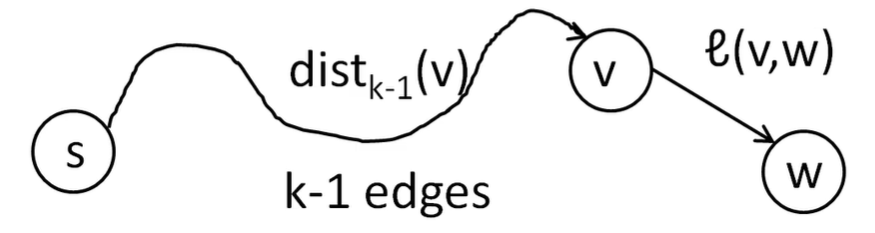
\includegraphics[scale=0.4]{assets/fun_sho_path_2.png}
\end{center}
If we look at a path from $s$ to $w$ with at most $k$ edges, this is a path from $s$ to $v$ that uses at most $k - 1$ edges for some $v$ plus a single edge from $v$ to $w$. The best length this path could have is $\text{dist}_{k - 1}(v) + \ell(v, w)$, where our $\text{dist}_{k - 1}(v)$ is minimized. 

\subsubsection{Bellman-Ford Algorithm}
This formula gives rise to the \emph{Bellman-Ford} algorithm. 
\begin{verbatim}
    Bellman-Ford(G, s, l)
        dist_{0}(v) = infinity for all v 
        dist_{0}(s) = 0
        For k = 1 to n
            For w in V
                dist_{k}(w) = min(dist_{k}(w), dist_{k - 1}(v) + l(v, w))
            dist_{k}(s) = min(dist_{k}(s), 0)
\end{verbatim}
We note that each iteration of the outer-loop is $\BigO(|E|)$ time. However, what value of $k$ do we use? 

\subsubsection{Example: Applying the Bellman-Ford Algorithm}
Find the shortest path from $s$ to every other vertex in the graph shown below. For convenience, let the top-left vertex be denoted $A$, the top-right vertex be $B$, and the bottom-right vertex be $C$. 
\begin{center}
    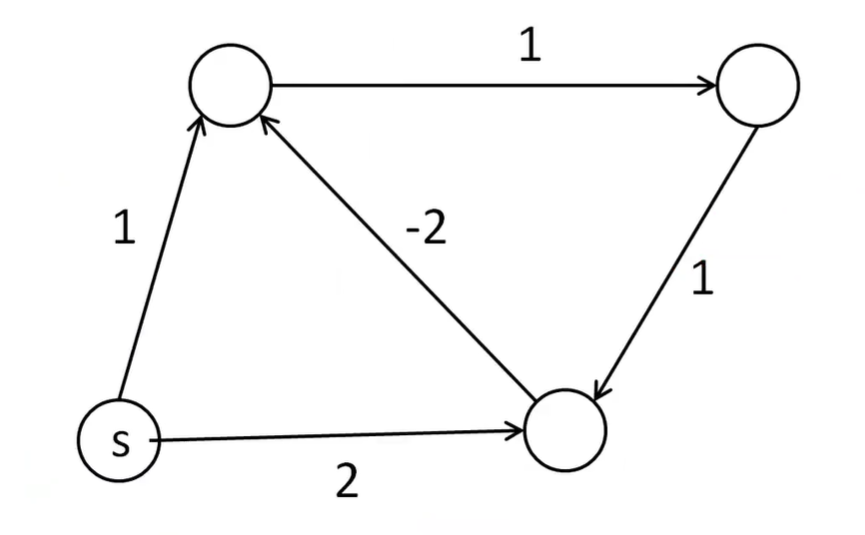
\includegraphics[scale=0.4]{assets/shortest_path_problem.png}
\end{center}

\begin{mdframed}[]
    \begin{itemize}
        \item First, when $k = 0$, $s = 0$ and everything else is assigned $\infty$; you can't get to anywhere else with no edges. Therefore, the distances are: 
        \begin{center}
            \begin{tabular}{c|c c c c}
                $k$ & $s$   & $A$       & $B$       & $C$ \\ 
                \hline 
                0   & 0     & $\infty$  & $\infty$  & $\infty$
            \end{tabular}
        \end{center}

        \item When $k = 1$, we consider all vertices that we can reach with one edge. So, you still can't reach vertex $B$ since it needs at least two edges. But, we can get from $s$ to $A$ with path length 1, and we can get from $s$ to $C$ with path length 2. So: 
        \begin{center}
            \begin{tabular}{c|c c c c}
                $k$ & $s$   & $A$       & $B$       & $C$ \\ 
                \hline 
                0   & 0     & $\infty$  & $\infty$  & $\infty$ \\ 
                1   & 0     & 1         & $\infty$  & 2
            \end{tabular}
        \end{center}
        In other words, these are the shortest distances we can get from a path of length one to each of our vertices. 

        \item When $k = 2$, we consider all vertices that we can reach with two edges. First, we can reach vertex $B$ with just two edges (from $s$ to $A$ and from $A$ to $B$). $A$ has distance 1 so $B$ must have distance 2. We can't do any better with $s$ or $C$, but note that we can actually improve $A$ (if we go from $s$ to $C$ and from $C$ to $A$) by getting it down to distance 0. Therefore: 
        \begin{center}
            \begin{tabular}{c|c c c c}
                $k$ & $s$   & $A$       & $B$       & $C$ \\ 
                \hline 
                0   & 0     & $\infty$  & $\infty$  & $\infty$ \\ 
                1   & 0     & 1         & $\infty$  & 2 \\ 
                2   & 0     & 0         & 2         & 2
            \end{tabular}
        \end{center}

        \item When $k = 3$, we consider all vertices that we can reach with three edges. So, we can again reach every vertex. In particular, note we can update vertex $B$'s distance. This is because if $A$ is 0, then there is a path from $A$ to $B$ that has length 1 ($s \to C \to A \to B$). So: 
        \begin{center}
            \begin{tabular}{c|c c c c}
                $k$ & $s$   & $A$       & $B$       & $C$ \\ 
                \hline 
                0   & 0     & $\infty$  & $\infty$  & $\infty$ \\ 
                1   & 0     & 1         & $\infty$  & 2 \\ 
                2   & 0     & 0         & 2         & 2 \\ 
                3   & 0     & 0         & 1         & 2
            \end{tabular}
        \end{center}

        \item Past $k = 3$, we notice that the distances no longer change. In other words, the process has stabilized. 
    \end{itemize}
\end{mdframed}

\subsubsection{Analysis}
\begin{proposition}
    If $n \geq |V| - 1$ and if $G$ has no negative weight cycles, then for all $v$,
    \[\text{dist}(v) = \text{dist}_{n}(v)\]
\end{proposition}
This says that if we run the Bellman-Ford algorithm, there is a limit. Assuming there are no negative weight cycles\footnote{If there is a negative weight cycle, there is probably no shortest path.}, we only need to run the algorithm for $|V| - 1$ rounds for a final runtime of $\BigO(|V||E|)$.

\begin{mdframed}[]
    \begin{proof}
        We need to show that the shortest path has fewer than $|V|$ edges. Suppose that there is a path that has at least $|V|$ edges, then by the pigeonhole principle, it must contain the same vertex twice. This means that there is a loop. If we remove the loop (which we assume has non-negative total weight, i.e. not a negative weight cycle), then we get a shorter path. This new path has at most $|V| - 1$ edges since we can only hit each vertex at most once. Note that this path is no longer than the one with the loop since we're considering the \emph{shortest} distance. 
    \end{proof}
\end{mdframed}

\subsubsection{Revised Bellman-Ford Algorithm}
With this analysis in mind, our algorithm looks like: 
\begin{verbatim}
    Bellman-Ford(G, s, l)
        dist_{0}(v) = infinity for all v 
        dist_{0}(s) = 0
        For k = 1 to |V|
            For w in V
                dist_{k}(w) = min(dist_{k}(w), dist_{k - 1}(v) + l(v, w))
            dist_{k}(s) = min(dist_{k}(s), 0)
        Return dist_{|V|}(t)
\end{verbatim}
Which we now know computes the shortest paths \emph{if no negative weight cycles} in $\BigO(|V||E|)$ time. 


\subsubsection{Detecting Negative Cycles}
\emph{If} there are no negative weight cycles, Bellman-Ford computes the shortest paths. Suppose there \emph{are} negative weight cycles. Well, Bellman-Ford will calculate some distances which will probably be garbage values.

\bigskip 

How do we know whether or not there are any negative weight cycles? 

\subsubsection{Negative Cycle Detection}
\begin{proposition}
    For any $n \geq |V| - 1$, there are \textbf{no} negative weight cycles reachable from $s$ if and only if, for every $v \in V$:
    \[\text{dist}_{n}(v) = \text{dist}_{n + 1}(v)\]
\end{proposition}
So, to detect negative cycles, all we need to do is run one more round of Bellman-Ford and see if any distances change. 

\begin{mdframed}[]
    \begin{proof}
        Suppose no negative weight cycles exist. Then, for any $n \geq |V| - 1$, $\text{dist}_{n}(v) = \text{dist}(v)$. So, $\text{dist}_{n}(v) = \text{dist}(v) = \text{dist}_{n + 1}(v)$ by the transitive property (since $n + 1 \geq n \geq |V| - 1$). 

        \bigskip 

        Suppose $\text{dist}_{n}(v) = \text{dist}_{n + 1}(v)$ for all $v$. Then: 
        \begin{equation*}
            \begin{aligned}
                \text{dist}_{n + 2}(w) &= \min_{(v, w) \in E} (\text{dist}_{n + 1}(v) + \ell(v, w)) \\ 
                    &= \min_{(v, w) \in E} (\text{dist}_{n}(v) + \ell(v, w)) \\
                    &= \text{dist}_{n + 1}(w)
            \end{aligned}
        \end{equation*}
        We essentially apply the idea that if $\text{dist}_{n}(v) = \text{dist}_{n + 1}(v)$, then the same idea holds for $n + 1$. In other words, if the distances are the same for one round from $n$ to $n + 1$, then it will be the same for $n + 1$ to $n + 2$ and so on. If the distance functions stabilize for one round, they will stabilize forever. So: 
        \[\text{dist}_{n}(v) = \text{dist}_{n + 1}(v) + \text{dist}_{n + 2}(v) + \text{dist}_{n + 3}(v) + \dots\]
        \emph{However}, if there were a negative weight cycle, the distances would decrease eventually. 
    \end{proof}
\end{mdframed}


\subsection{Problem: Finding Shortest Paths in DAGs (With Arbitrary Edge Weights)}
We saw that shortest paths is harder when we needed to deal with negative weight cycles. For general graphs, we needed to use Bellman-Ford which is much slower than our other algorithms. In our case here, if we're working with a DAG, then there are faster algorithms that we can apply. 

\bigskip 

Recall that, for any vertex $w$ that isn't the source $s$, $w \neq s$,
\[\text{dist}(w) = \min_{(v, w) \in E} \text{dist}(v) + \ell(v, w)\]
We can use topological ordering for DAGs to compute the shortest distance.

\subsubsection{Algorithm}
The algorithm is as follows: 
\begin{verbatim}
    ShortestPathsInDAG(G, s, l)
        TopologicalSort(G)
        For w in V in topological order
            If w = s
                dist(w) = 0
            Else
                dist(w) = min(dist(v) + l(v, w))
\end{verbatim}
This has runtime $\BigO(|V| + |E|)$. 



\subsection{Shortest Path Algorithms Summary}
\begin{center}
    \begin{tabular}{p{3in}|p{1.5in}|p{1.5in}}
        \textbf{Path Type} & \textbf{Algorithm} & \textbf{Runtime} \\ 
        \hline 
        Unit Weights, General Graph & \code{Breadth First Search} & $\BigO(|V| + |E|)$ \\ 
        Non-Negative Weights, General Graph & \code{Dijsktra} & $\BigO(|V|\log(|V|) + |E|)$ \\ 
        Arbitrary Weights, General Graph & \code{Bellman-Ford} & $\BigO(|V||E|)$ \\ 
        Arbitrary Weights, DAG & \code{ShortestPathsInDAG} & $\BigO(|V| + |E|)$
    \end{tabular}
\end{center}


















\newpage 
\section{Divide and Conquer}
The idea behind divide and conquer is as follows: 
\begin{enumerate}
    \item \underline{Divide:} Break the given problem into similar pieces (i.e. subproblems of same type). This step involves breaking the problem into smaller sub-problems. Sub-problems should represent a part of the original problem. This step generally takes a recursive approach to divide the problem until no sub-problem is further divisible.
    \item \underline{Conquer:} Recursively solve these pieces (sub-problems). This step receives a lot of smaller sub-problems to be solved. Generally, at this level, the problems are considered 'solved' on their own.
    \item \underline{Combine:} Appropriately combine the answers. When the smaller sub-problems are solved, this stage recursively combines them until they formulate a solution of the original problem.
\end{enumerate}

\subsection{Problem: Integer Multiplication}
Suppose we're given two $n$-bit binary numbers and are asked to find their product. 

\subsubsection{Naive Algorithm}
The naive algorithm is to do multiplication like we would from elementary school. This runs in $\BigO(n^2)$ time because we need to write down $\BigO(n^2)$ bits of numbers to add (addition is done in linear time and is omitted).

\subsubsection{Improving the Algorithm: Two-Digit Multiplication}
Suppose we tried to multiply $ab$ by $cd$. This is normally done like so: 
\begin{verbatim}
                        a           b
                    x   c           d
                        -------------
                        ad         bd 
            +   ac      bc          0
                ---------------------
                ac      ad+bc      bd 
\end{verbatim}
This requires 4 one-digit multiplications and one addition. The \textbf{trick} is to compute $ac$, $bd$, $(a + b)(c + d)$. We note that (\emph{digit-wise}): 
\[bc + ad = (a + b)(c + d) - ac - bd\]
This requires \emph{3} one-digit multiplications and 4 addition/subtractions.

\subsubsection{Improving the Algorithm: Larger Base}
We can essentially generalize the above to larger bases with more digits. For example:
\begin{verbatim}
                a1      a2      a3   ...a(n/2)      a(n/2 + 1)   ...an
            x   b1      b2      b3   ...b(n/2)      b(n/2 + 1)   ...bn
                ------------------------------------------------------
                AC                      AD + BC                     BD 
\end{verbatim}
Where we can split the digits so that $A$ takes the first half of the first number, $B$ takes the second half of the first number, $C$ takes the first half of the second number, and $D$ takes the second half of the second number. 

\subsubsection{Formally}
Suppose we wanted to multiply $N$ by $M$. Then: 
\begin{enumerate}
    \item Let $X \approx \sqrt{N + M}$ be a power of 2. 
    \item Write $N = AX + B$ and $M = CX + D$. This can be done by just taking the high and low bits. 
    \item $NM = ACX^2 + (AD + BC)X + BD = ACX^2 + ((A + B)(C + D) - AC - BD)X + BD$, where the multiplication by $X$ are just bit shifts. 
\end{enumerate}

\subsubsection{Algorithm}
\begin{verbatim}
    ImprovedMult(N, M):
        Let X be 2^(log(N + M) / 2)
        Write N = AX + B, M = CX + D 
        P1 = Product(A, C)
        P2 = Product(B, D)
        P3 = Product(A + B, C + D)
        Return P1 X^2 + [P3 - P1 - P2]X + P3
\end{verbatim}
The first two lines take $\BigO(n)$ time, the three \code{Product} calls take $\BigO(n^2)$, and the last step takes $\BigO(n)$, for a total runtime of $\BigO(n^2)$. Despite there not being an asymptotic difference, note that this algorithm runs in $\BigO\left(\frac{3}{4}n^2 + n\right)$ time, whereas the naive algorithm runs in $\BigO(n^2)$ time, so there is a slight improvement. 

\subsubsection{Further Improvements}
Our algorithm still uses the naive algorithm (\code{Product}). However, we don't actually need to use this; we can just use our own implementation! We introduce \emph{Karatsuba's Algorithm}.

\begin{verbatim}
    KaratsubaMult(N, M)
        If N + M < 99
            Return Product(N, M)
        Let X be 2^(log(N + M) / 2)
        Write N = AX + B, M = CX + D 
        P1 = KaratsubaMult(A, C)
        P2 = KaratsubaMult(B, D)
        P3 = KaratsubaMult(A + B, C + D)
        Return P1 X^2 + [P3 - P1 - P2]X + P3
\end{verbatim}
Here, the pre-processing and post-processing still takes $\BigO(n)$ time. The three recursive calls are a bit tricky. 

\subsubsection{Runtime Recurrence}
Karatsuba's multiplication on inputs of size $n$ spends $\BigO(n)$ time, and then makes three recursive calls to problems of approximately half the size. If $T(n)$ is the runtime for $n$-bit inputs, we have the recurrence:
\[T(n) = \begin{cases}
    \BigO(1) & n = \BigO(1) \\ 
    3T(n / 2 + \BigO(1)) + \BigO(n) & \text{Otherwise}
\end{cases}\]
This isn't exactly a clean recurrence that we can solve. That being said, this runs in roughly $\BigO(n^{\log_{2}(3)})$ time. We will explain this later. 

\subsection{Generalization \& Master Theorem}
We will often get runtime recurrences with divide and conquer looking something like: 
\[T(n) = \begin{cases}
    \BigO(1) & n = \BigO(1) \\ 
    aT\left(\frac{n}{b} + \BigO(1)\right) + \BigO(n^d) & \text{Otherwise}
\end{cases}\]
Here, the second line is saying $a$ subproblems of size $\frac{n}{b}$. Note that the recursive subcalls are a constant \emph{fraction} of the size of the original. For example, if $T(n) = 2T(n - 1)$, then $T(n) = \BigO(2^n)$. 

\subsubsection{Tracking Recursive Calls}
We have: 
\begin{itemize}
    \item 1 recursive calls of size $n$
    \item $a$ recursive calls of size $n / b + O(1)$
    \item $a^2$ recursive calls of size $n / b^2 + O(1)$
    \item \dots
    \item $a^k$ recursive calls of size $n / b^k + O(1)$
\end{itemize}
So, the total runtime is: 
\begin{equation*}
    \begin{aligned}
        \text{Total Runtime } &= \sum_{k = 0}^{\log_{b}(n)} a^k \BigO\left(\left(\frac{n}{b^k}\right)^d\right) \\ 
            &= \BigO(n^d) \sum_{k = 0}^{\log_{b}(n)} \left(\frac{a}{b^d}\right)^k
    \end{aligned}
\end{equation*}

There are several cases to consider. 
\begin{enumerate}
    \item $a > b^d$: Increasing geometric series dominated by last term. The runtime is dominated by recursive calls at the bottom level. The runtime would be $O(n^{\log){b}(a)})$.
    \item $a < b^d$: Decreasing geometric series is dominated by the first term. Rutime is mostly based on the cleanup steps at the top level. The runtime is $O(n^d)$. 
    \item $a = b^d$: Every level of the recursion does the same amount of work. The runtime is $O(n^d \log(n))$. 
\end{enumerate}

\subsubsection{Master Theorem}
\begin{theorem}{Master Theorem}{}
    Let $T(n)$ be given by the recurrence:
    \[T(n) = \begin{cases}
        \BigO(1) & n = \BigO(1) \\ 
        aT\left(\frac{n}{b} + \BigO(1)\right) + \BigO(n^d) & \text{Otherwise}
    \end{cases}\]
    Then we have: 
    \[T(n) = \begin{cases}
        \BigO(n^{\log_{b}(a)}) & a > b^d \\ 
        \BigO(n^d \log(n)) & a = b^d \\ 
        \BigO(n^d) & a < b^d
    \end{cases}\]
\end{theorem}

\subsubsection{Example: Runtime}
Suppose that a divide and conquer algorithm needs to solve 4 recursive subproblems of half the size and do $\BigO(n^2)$ addition work. What is the runtime? 
\begin{mdframed}[]
    Here, we have 4 subproblems ($a = 4$) of half the size ($b = 2$) and we need to do $\BigO(n^2)$ additional work ($d = 2$). So, our recurrence is given by 
    \[T(n) = \begin{cases}
        \BigO(1) & n = \BigO(1) \\ 
        4T\left(\frac{n}{2} + \BigO(1)\right) + \BigO(n^2) & \text{Otherwise}
    \end{cases}\]
    Since $b^d = 2^2 = 4$ and $a = b^d$, it follows that the runtime is 
    \[\BigO(n^2 \log(n))\]
\end{mdframed}


\subsection{Problem: Matrix Multiplication}
Suppose we wanted to multiply $n \times n$ matrices.

\subsubsection{Recall}
If $AB = C$, then 
\[C_{i, j} = \sum_{k} A_{i, k} B_{k, j}\]
The naive algorithm computes this sum of $n$ terms for each of $n^2$ entries, so the runtime is given by $\BigO(n^3)$.

\subsubsection{Block Matrix Multiplication}
If we divide the matrix into blocks, we can get the product of the full matrix in terms of the products of the blocks. 
\[
    \begin{bmatrix}
        A & B \\ C & D
    \end{bmatrix} \begin{bmatrix}
        E & F \\ G & H
    \end{bmatrix} = \begin{bmatrix}
        AE + BG & AF + BH \\ 
        CE + DG & CF + DH 
    \end{bmatrix}
\]
Here, $A, B, C, \dots$ are $(n / 2) \times (n / 2)$ matrices. 

\subsubsection{Divide and Conquer Algorithm}
We can compute 8 products of $(n / 2) \times (n / 2)$ matrices, and do some addition to get an answer. The runtime is 
\[T(n) = 8T(n / 2) + \BigO(n^2)\]
The Master Theorem states that this would give us $\BigO(n^3)$ runtime. And, this isn't hard to see why. If we unrolled what this algorithm was doing, we're essentially just doing the naive multiplication.



\subsection{Problem: Sorting}
Given a list $L$ of numbers, return $L$ in sorted order.

\subsubsection{Algorithm Idea}
An idea is to: 
\begin{itemize}
    \item Divide $L$ into two parts, $L_1$ and $L_2$. 
    \item Sort $L_1$ and $L_2$. 
    \item Finally, \emph{merge} both $L_1$ and $L_2$ together. 
\end{itemize}

\subsubsection{Merge Operation}
One question we have is, how do we define the \emph{merge} operation? Well, suppose we have
\[L_1 = [1, 3, 6, 10]\]
\[L_2 = [2, 4, 5, 7, 8, 9]\]

We can combine the two lists by comparing the two smallest elements an then putting the smaller of the two elements in the new list. So, for example, the first element in $L_1$ is 1 and the first element in $L_2$ is 2, so we can put $1$ into the final list and somehow point $L_1$ to the second element so we don't consider $1$ again. Then, we can consider $3$ in $L_1$ and $2$ in $L_2$; in this case, we put $2$ into the final list and point $L_2$ to the second element so we don't consider $2$ again. We can keep doing this until we go through every element in both parts of the list. 

\bigskip 

The algorithm can be described like so: 
\begin{verbatim}
    Merge(A, B):
        Let C be the list with the length being len(A) + len(B)
        // Kane uses one-indexing instead of zero-indexing.
        a = 1 
        b = 1
        for c = 1 to len(C):
            if b > len(B)
                C[c] = A[a]
                a++ 
            else if a > len(A)
                C[c] = B[b]
                b++ 
            else if A[a] < B[b]
                C[c] = A[a]
                a++ 
            else 
                C[c] = B[b]
                b++ 
        Return C
\end{verbatim}
This runs in $\BigO(|A| + |B|)$ time, particularly due to the \code{for}-loop. 

\subsubsection{Merge Sort Algorithm}
\begin{verbatim}
    MergeSort(L):
        // Every divide & conquer algorithm needs a base case 
        if len(L) == 1:
            return L
        
        Split L into approx. equal lists L1, L2
        return Merge(MergeSort(L1), MergeSort(L2))
\end{verbatim}

To analyze the runtime, we note the following:
\begin{itemize}
    \item \underline{Base Case:} The base case runs in $\BigO(1)$ time; this is obvious (and is expected for any base case).
    \item \underline{Divide \& Conquer:} The divide and conquer part comes in several steps. 
    \begin{itemize}
        \item \underline{Divide:} We divide our list $L$ into approximately equal-sized lists $L_1$ and $L_2$. We assume that this takes $\BigO(1)$ time. 
        \item \underline{Conquer:} It takes $2T(n / 2 + \BigO(1))$ time to recursively solve two subproblems, each of size $\frac{n}{2}$. The $\BigO(1)$ is due to the possibility that one of the two lists may have unequal sizes (e.g. one sublist has size 5 and another sublist has size 6). At the end of the day, we can just simplify this down to $2T(n / 2)$. 
        \item \underline{Combine:} Merging an $n$-element sublist takes $\BigO(n)$ time. This term absorbs the $\BigO(1)$ time from the divide part of the algorithm.  
    \end{itemize}
\end{itemize}
We then have (by the Master Theorem):
\[T(n) = 2T(n / 2) + \BigO(n)\]
Note that $a = 2$, $b = 2$, and $d = 1$, so the final runtime is given by the Master Theorem:
\[\BigO(n\log n)\]

\subsection{Problem: Order Statistics}
Given a list of numbers $L$, find the \textbf{median} or the \textbf{largest element} or the \textbf{10th smallest} element of $L$. Essentially, you want to find something based on the order in some way.

\bigskip 

Let's focus on one particular problem: Given $L$ and $k$, find the $k$th smallest element of $L$. 

\subsubsection{Easy Algorithm}
The easy algorithm is to sort $L$ and then return $L[k]$. The runtime is $\BigO(n \log n)$, but there are better ways to do this. 

\subsubsection{The Idea for the Divide Step}
First, we pick a \emph{pivot} $x \in L$ at random here, and we sort all elements in $L$ relative to $x$. That is, every element to the \emph{left} of $x$ is less than $x$, every element to the \emph{right} of $x$ is greater than $x$, and every element in the center is equal to $x$. In other words: 
\begin{verbatim}
                                           L = x
                                        ------------
    ------------------------------------            ------------------------------------
            L < x                                                         L > x
\end{verbatim}
In this sense, we can sort these elements into categories in $\BigO(n)$ time. Then: 
\begin{itemize}
    \item We note that the $k$th smallest element is less than $x$ if and only if $|L_{< x}| \geq k$. If this is the case, then the answer is the $k$th smallest element of $L_{< x}$. 
    \item The answer is $x$ if and only if $|L_{< x}| < k$ and $|L_{< x}| + |L_{= x}| \geq k$.
    \item Otherwise, the answer is the $(k - |L_{< x}| - |L_{= x}|)$th smallest in $L_{> x}$. 
\end{itemize}

\subsubsection{Divide and Conquer Algorithm}
\begin{verbatim}
    OrderStats(L, k)
        Pick x in L randomly 
        Sort into L[<x], L[=x], L[>x]
        If len(L[<x]) >= k
            return OrderStats(L[<x], k)
        else if len(L[<x]) + len(L[=x]) >= k
            return x 
        else 
            return OrderStats(L[>x], k - len(L[<x]) - len(L[=x]))
\end{verbatim}
The idea is that we use randomization to improve our runtime. If we didn't pick a random $x \in L$, then it's very possible that the $x$ that we pick is the smallest or biggest $x$, which means we would essentially have to consider $n - 1$ elements, and thus we would have a divide algorithm that takes $T(n - 1)$ time (and so $\BigO(n^2)$ time). By randomly selecting an $x \in L$
\begin{itemize}
    \item There is a 50\% chance that $x$ is selected in the middle half. 
    \item If so, no matter where the answer is, the recursive call is at most $3n / 4$. 
    \item On average, we might need two tries to reduce calls. 
\end{itemize}
The idea behind the $3n / 4$ is that, when we pick this $x$, we either recurse on everything bigger than $x$ or smaller than $x$. Because $x$ is in this middle half, there are at least $n / 4$ elements on either sides: 
\begin{verbatim}
        n / 4                             n / 2                                 n / 4  
    -----------------|--------x---------------------------------------|-----------------
\end{verbatim}
So, we have the runtime 
\[T(n) = \BigO(n) + T(3n / 4)\]
By the Master Theorem, we get the \emph{expected}  
\[\BigO(n)\]


\subsection{Problem: Searching Problem}
Given a sorted list $L$ and a number $x$, find the location of $x \in L$.

\subsubsection{Naive Algorithm}
The naive algorithm is to iterate over each element in $L$ and see where $x$ is in $L$. This takes $\BigO(n)$ time as the element in question might be at the end of the list.  

\bigskip 

\textbf{Remark:} Usually, you cannot beat $\BigO(n)$ because any algorithm needs to read the entire input. \emph{However}, since the list is guaranteed to be sorted, we can do better.

\subsubsection{Algorithm Idea}
First, we want to split $L$ into two sublists. The idea is to take advantage of the fact that $L$ is sorted to see which of the two sublists we should check. Essentially:
\begin{itemize}
    \item If $L[i] > x$, then the location must be before $i$.
    \item If $L[i] < x$, then the location must be after $i$. 
    \item If $L[i] = x$, then we found it. 
\end{itemize}
Of course, we don't want to actually \emph{split} the list; that would take too much time. Instead, we can have two indices $i$ and $j$ which determine which part of the list to check. 

\subsubsection{Divide and Conquer Algorithm}
\begin{verbatim}
    // Search between L[i] and L[j]
    BinarySearch(L, i, j, x)
        // This is the base case. 
        if j < i
            return 'error'
        k = (i + j) / 2
        if L[k] == x
            return k
        if L[k] > x
            return BinarySearch(L, i, k - 1, x)
        if L[k] < x 
            return BinarySearch(L, k + 1, j, x)
\end{verbatim}
To analyze the runtime, we note the following:
\begin{itemize}
    \item \underline{Base Case:} The base case runs in $\BigO(1)$ time; this is obvious (and is expected for any base case).
    \item \underline{Divide \& Conquer:} The divide and conquer part comes in several steps. 
    \begin{itemize}
        \item \underline{Divide:} The divide part comes from the calculation of $k$, which determines what range we want to consider when recursively calling \code{BinarySearch}.
        \item \underline{Conquer:} We're only interested in running through a \emph{subset} of $L$. Recall that, with binary search, while we're still working with the big list $L$, the range that we check will always be half of the previous range that was considered. With this in mind, it takes $T(n / 2 + \BigO(1))$ time to recursively solve one subproblem of size $\frac{n}{2}$. The $\BigO(1)$ is due to the possibility that one of the two ranges may have unequal sizes (e.g. one range covers 5 elements and another range has covers 6). At the end of the day, we can just simplify this down to $T(n / 2)$. 
        \item \underline{Combine:} Combining the answer is as simple as returning $k$. 
    \end{itemize}
\end{itemize}
We then have (by the Master Theorem):
\[T(n) = T(n / 2) + \BigO(n)\]
Note that $a = 1$, $b = 2$, and $d = 0$, so the final runtime is given by the Master Theorem:
\[\BigO(\log n)\]


\subsubsection{Puzzles \& Applications}
\begin{mdframed}[]
    Binary search, or something related to that, occurs when we try to solve a problem with a finite number of possible answers and, every time we make a guess as to what the answer is, we eliminate a \emph{constant fraction} of the possibilities. \textbf{Put it another way}, lots of puzzles have binary search-like answers; as long as you can spend \emph{constant time} to divide your search space by some constant fraction, you can use binary search in $\BigO(\log(n))$ time.  
\end{mdframed}
Suppose you have 27 coins, one of which is \emph{heavier} than the others, and a balance. You are asked to determine the heavy coins in 3 weighings. The idea is: 
\begin{itemize}
    \item After one weighing, you're down to 9 possibilities. 
    \item After another weighing, you're down to 3 possibilities.
    \item After a third weighing, you're down to just 1 possibility. 
\end{itemize}


\subsection{Problem: Closest Pair of Points}
Given $n$ points in the plane, $(x_1, y_1), \dots, (x_n, y_n)$, find the pair $(x_i, y_i)$ and $(x_j, y_j)$ whose Euclidean distance is as small as possible. 

\subsubsection{Naive Algorithm}
The naive algorithm is to simply try every pair of points. This runs in $\BigO(n^2)$ time; you have $n$ points so $n^2$ possibilities. 

\subsubsection{Divide and Conquer Outline}
In order to use divide and conquer, you need to find some way to divide the set of points into two equally sized subsets. One reasonable way to do this is to draw a line and cut the plane so that you can consider the points on the left and right of the line. 
\begin{center}
    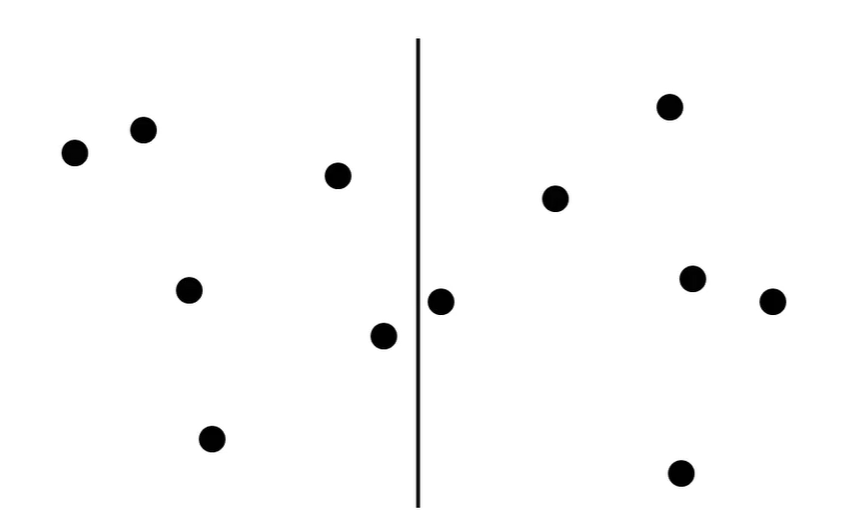
\includegraphics[scale=0.2]{assets/closest_pts_1.png}
\end{center}
From there, you can compute the closest pair of points on each side. 
\begin{center}
    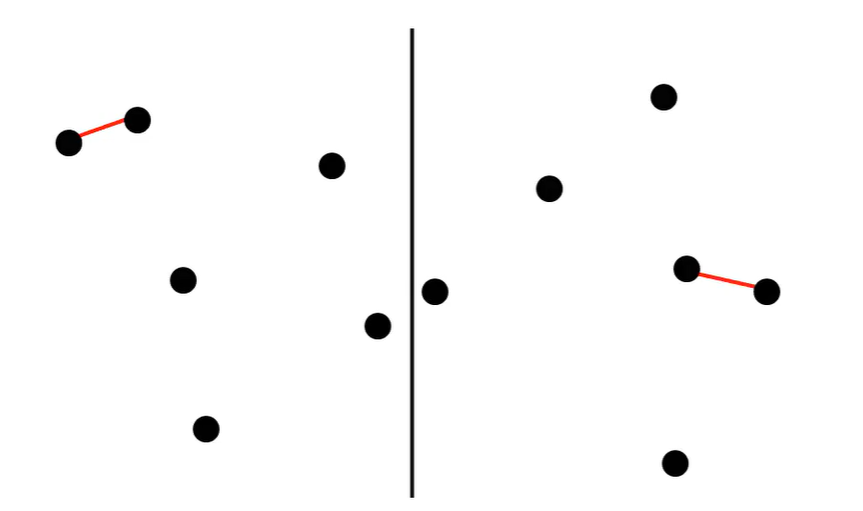
\includegraphics[scale=0.2]{assets/closest_pts_2.png}
\end{center}
After we do this, we need to somehow recombine the answers to our subproblems so we can get the answer. \textbf{However}, we can't simply just return the better of the two pairs (denoted by the red line) because it's possible that the best pair of points actually \emph{crosses} the line that we used to cut our problem in half (which we didn't consider since these two points are in separate subsets). So, what do we do? 

\subsubsection{Observation}
Consider the following set of points, with the dividing line: 
\begin{center}
    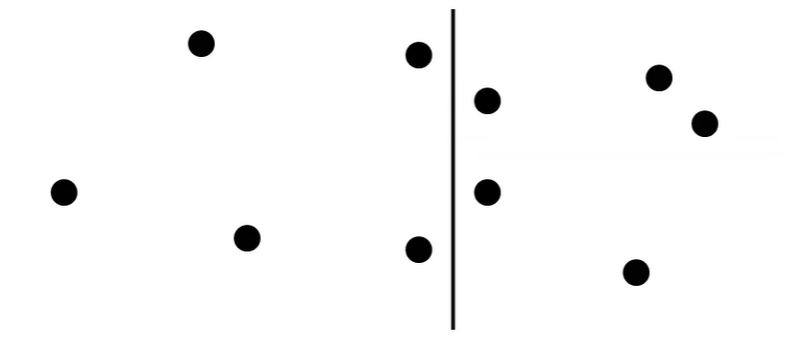
\includegraphics[scale=0.3]{assets/closest_pts_3.png}
\end{center}
Suppose that the closest pair of points on \emph{either side} of the dividing line is at distance $\delta$; that is, two points on the same side has distance $\delta$. 
\begin{center}
    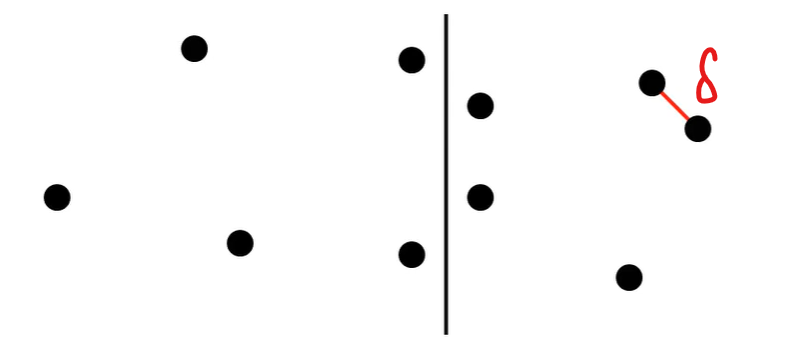
\includegraphics[scale=0.3]{assets/closest_pts_4.png}
\end{center}
At the very least, we only need to care about points \emph{within} $\delta$ of the dividing line. So, we only need to consider a \emph{strip} of width $2\delta$:
\begin{center}
    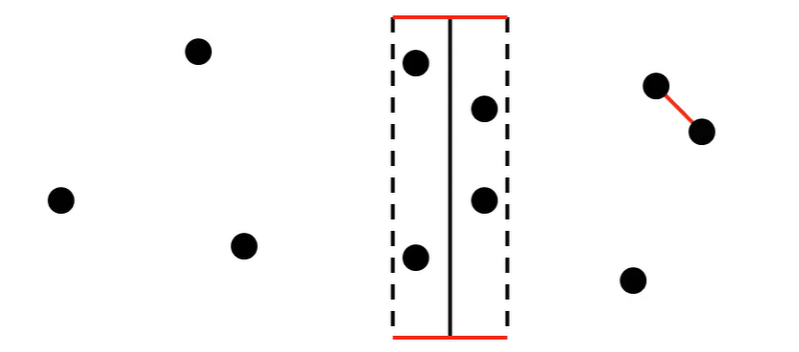
\includegraphics[scale=0.3]{assets/closest_pts_5.png}
\end{center}
In our case here, we now only focus our attention on any points within this strip. We now need to know if there is some pair of points in this strip where the distance between the points in that pair is \emph{less than} $\delta$. In other words, is there a pair of points in this strip whose distance is \emph{better} than the distance that we already found (i.e. $\delta$)?


\subsubsection{Main Idea}
The main idea is that we know that any pair of points on the same side of the line has to be separated by at least $\delta$. So, the points inside this strip must be reasonably spaced out vertically. So, if we want to find some pair of points that are closer to $\delta$, there can't be that many other points in between them. If we sort the points vertically (by their $y$-coordinates), then two points that are super close to each other cannot be far off in that ordering. 
\begin{proposition}
    Take the points within $\delta$ of the dividing line and sort them by $y$-coordinate. Any one of these points can only be within $\delta$ of the 8 closest points on either side of it. 
\end{proposition}
So, sort everything by $y$-coordinate. Then, look at the next 8 points\footnote{What really matters is that this is \textbf{some constant}; it can be 5 or 10 or 127 or whatever.} in $y$-coordinate above it and the next 8 points in $y$-coordinate below it. Those are the only possible points that can possibly be within $\delta$ of the point that we're considering. 

\bigskip 

If the proposition is true, then this means we only need to check a few pair of points crossing the line. The \emph{idea} is that the points on each side of the line are separated by at least $\delta$. This is because we know that $\delta$ is the distance to the closest pair of points for any pair of points on either side of the line. This means that there isn't enough room to cram many points into a narrow region because this forces points to be spread out. 

\begin{mdframed}[]
    \begin{proof}
        Suppose we have the dividing line, some $\delta$, and a point.
        \begin{center}
            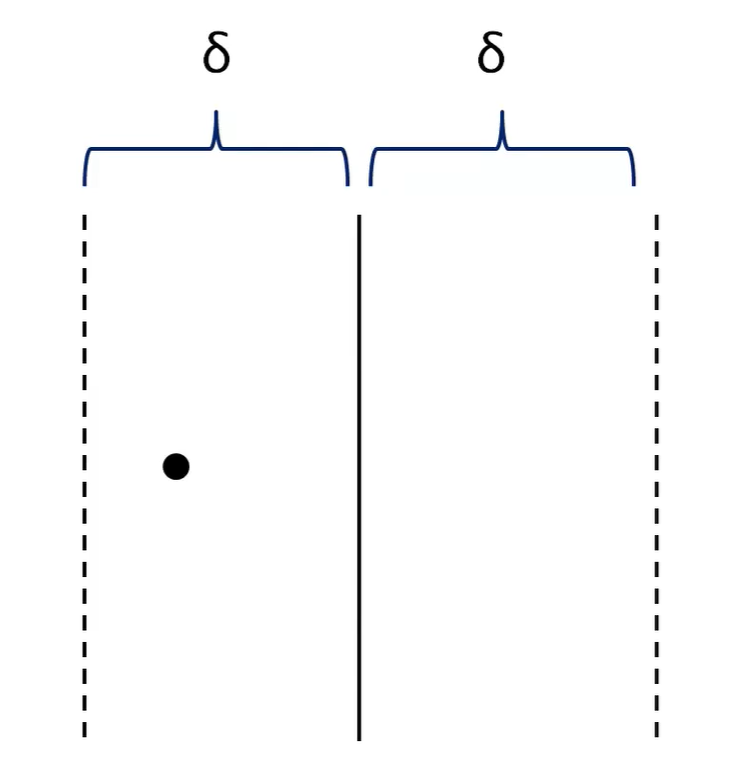
\includegraphics[scale=0.37]{assets/closest_proof_1.png}
        \end{center}
        Any nearby point has to be within this strip and the $y$-coordinate of that point we're looking for must be within $\delta$ of the $y$-coordinate that we have. So, we can create a bigger box and every other point that we want to match this one point with must be somewhere in this box.
        \begin{center}
            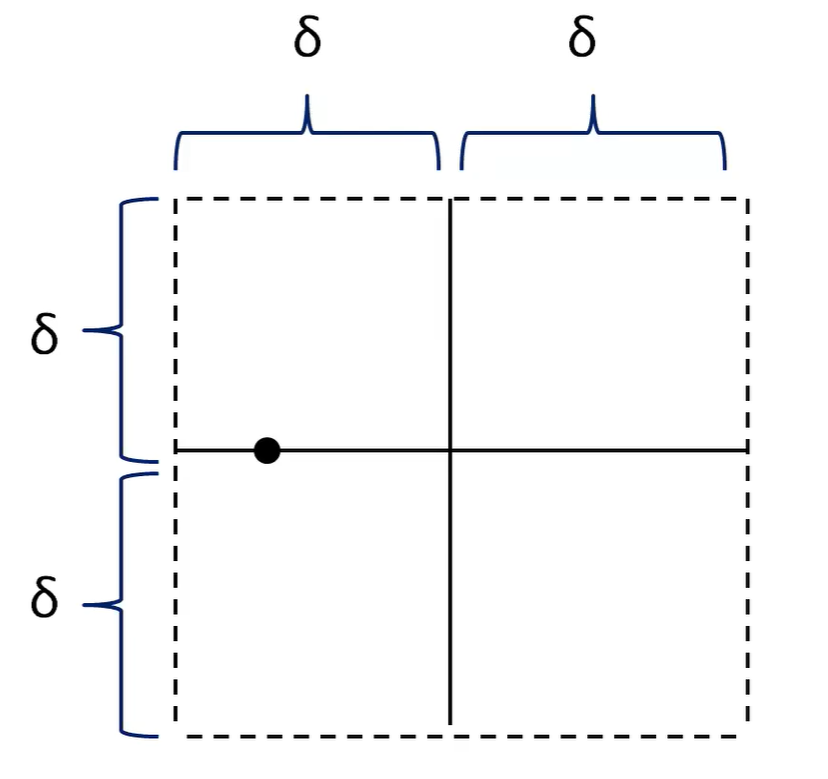
\includegraphics[scale=0.37]{assets/closest_proof_2.png}
        \end{center}
        So, we can subdivide this region into $\delta / 2$-sided squares. 
        \begin{center}
            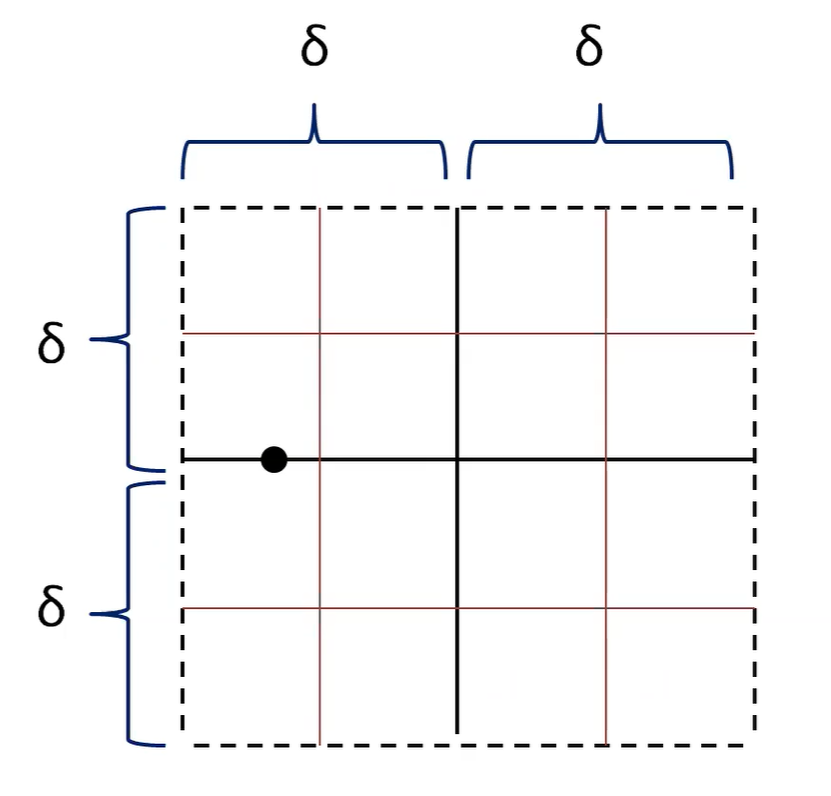
\includegraphics[scale=0.37]{assets/closest_proof_3.png}
        \end{center}
        There are now 16 squares; 8 of them are above the point and 8 of them are below the point. The claim is that each of these little squares can have at most one point. This is because if we take any two points inside the same square, the distance between those points will be less than $\delta$. In particular, since every square is either on the left or right side of the dividing line, we can't have two points in the same square with distance less than $\delta$ because then there would be points on the same side of the dividing line with distance less than $\delta$. 
        \begin{center}
            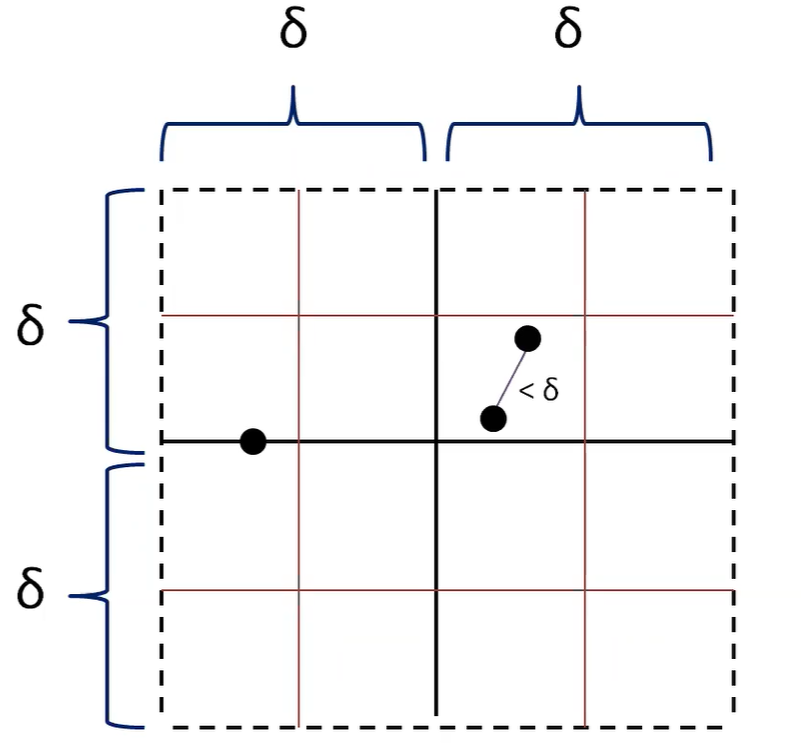
\includegraphics[scale=0.37]{assets/closest_proof_4.png}

            \textbf{Figure:} Two points in the same square with distance less than $\delta$, a contradiction to our original claim that $\delta$ was the smallest distance between two points on the same side of the line. 
        \end{center}
        
        So, the point is that there is at most one point in each square\footnote{Note that there is a possibility that there is a point on the dividing line. In this case, just move the dividing line until there are no points on it. Alternatively, we can treat points on the line as being on the left/right of the dividing line.}. Thus, there are at most 8 points below and above our given point; any other points close to our given point must be farther than $\delta$ or outside of the strip. This completes the proof. 
    \end{proof}
\end{mdframed}

\subsubsection{The Algorithm}
\begin{verbatim}
    CPP(S)
        // Base case, brute force it. 
        If len(S) <= 3
            return closest distance 
        
        Find line L evenly dividing points.                     // (a)
        Sort S into S_{left}, S_{right}                         // (b)
        // D is delta 
        let D = min(CPP(S_{left}), CPP(S_{right}))              // (c)
        let T be the points within D of L                       // (d)
        Sort T by y-coordinate                                  // (d)
        Compare each element of T to 8 closest on either side.  // (e)
            Let min dist be D' 
        Return min(D, D')
\end{verbatim}

The runtime analysis is as follows: 
\begin{enumerate}[\hspace{0.5cm}(a)]
    \item First, finding the line that evenly divides the points take $\BigO(n)$ time. 
    \item Sorting the points into the two sets takes $\BigO(n)$ time. 
    \item The two recursive calls take $2T(n / 2)$ time. 
    \item Finding and sorting $T$ takes $\BigO(n\log(n))$ time. 
    \item Comparing each element of $T$ to 8 closest on either side takes $\BigO(n)$ time. 
\end{enumerate}
This gives us the recurrence: 
\[T(n) = \BigO(n\log(n)) + 2T(n / 2)\]
This is not a runtime recurrence that we can use the Master Theorem for; this is particularly because the Master Theorem uses $\BigO(n^d)$ whereas we have $\BigO(n\log(n))$. However, by running a Master Theorem-like argument, we have that 
\[T(n) = \BigO(n\log^{2}(n))\]
Alternatively, if we are more careful and have \code{CPP} take points already sorted by $y$-coordinate, we can reduce this runtime down to $\BigO(n\log(n))$. 






















\newpage 
\section{Greedy Algorithms}
A greedy algorithm is an algorithm where you want to build up some solution one step at a time. At every step, you come up with some notion of what the \emph{best} choice you can make is, and make that choice; in other words, at every step, you make the \emph{best available choice} until you can no longer make any choices. 

\bigskip 

A few things to keep in mind regarding greedy algorithms:
\begin{itemize}
    \item They are very simple (almost trivial) and clean to write. \emph{When they work}, they tend to be very good algorithms. 
    \item It's not uncommon to write a greedy algorithm that seems to work, but actually fails. Thus, proving correctness is very important. 
\end{itemize}

\subsection{Problem: Making Change}
Given some amount of money (in US dollars), you want to make the exact change for it using as few bills and coins as possible. For example, if we wanted to make change for a single dollar, you would use a single dollar bill instead of 100 pennies. 

\subsubsection{Greedy Algorithm}
The algorithm is to repeatedly add the biggest denomiation still available.

\subsubsection{Example: Making Change}
What is the most optimal way to make change for \$12.73? Here, we define optimal as using the least number of bills and coins to make exact chamge. 

\begin{mdframed}[]
    Suppose we wanted to make change for \$12.73. 
    \begin{itemize}
        \item We can begin with a change for \$10 bill, so we now need to make change for \$2.73.
        \item We can next use two \$1 bills, so we now need to make change for \$0.73. 
        \item Next, we can use two quarters, so we now need to make change for \$0.23.
        \item Next, we can use two dimes, so we now need to make change for \$0.03.
        \item Finally, we can use three pennies. 
    \end{itemize}
    At the end, we only needed 10 different bills and coins to make change.
\end{mdframed}


\subsubsection{Result}
\begin{proposition}
    For standard US currency denomiations, this algorithm is always optimal. 
\end{proposition}

\begin{mdframed}[]
    \begin{proof}
        This proof is omitted. 
    \end{proof}
\end{mdframed}

\subsubsection{Non-Application to Other Currencies}
This property does not necessarily hold for other currencies. 

\bigskip 

For example, suppose we have a country with currency $W$, where the denominations are $7W$, $5W$, and $1W$. What if we try to make change for $10W$?
\begin{itemize}
    \item We first use $7W$, leaving us with $3W$ left to make change. 
    \item Then, we use three $1W$ to cover the rest of the change needed. 
\end{itemize}
This leaves us with 4 different bills and coins. However, the optimal solution is actually to use two $5W$ instead. 


\subsection{Problem: Interval Scheduling}
You are trying to figure out your classes for the next quarter, and you are at a school where classes have weird times (e.g. 3:15 PM to 3:27 PM). You're not allowed to pick two classes that overlap. However, beyond this, you are a masochist and so you want to schedule as many classes as you possibly can; you don't care what classes you want to take, just that you can take them without having any overlaps.

\bigskip 

More formally, given a set $S$ of intervals $[x_i, y_i] = I_i$, you want to find a subset $T \subseteq S$ such that
\begin{enumerate}
    \item No two intervals in $T$ overlap. 
    \item Subject to condition 1, $|T|$ should be as large as possible. 
\end{enumerate}
For example, if we have the following intervals:
\begin{verbatim}
    |----------------------|
        |-----| |------------|
      |------| |-------| |------|
\end{verbatim}
It's not hard to see that the answer would be the three bottom intervals. 

\subsubsection{Greedy Algorithm Idea}
We want to build this schedule one interval at a time. Now, we want to figure out which intervals we should be adding. Some ideas include: 
\begin{itemize}
    \item Shortest intervals, because longer intervals are more expensive to add. 
    \item Fewest overlaps. 
    \item Ends soonest. 
    \item Starts soonest. 
\end{itemize}
Picking the shortest interval doesn't work; consider this counterexample, where the two longest intervals represent the best possible solution:
\begin{verbatim}
    |-----------------------------| |-----------------------------------|
                                |-----|
\end{verbatim}
Picking the intervals with fewest overlaps doesn't work; consider this counterexample, where picking the interval with the fewest overlaps locks ourselves from the best possible schedule: 
\begin{verbatim}
    |------| |------| |------| |------|
        |-------| |------| |-------|
        |-------|          |-------|
        |-------|          |-------|
        |-------|          |-------|
\end{verbatim}
Picking the intervals that start the soonest also doesn't work; consider this counterexample, where picking the interval that starts the soonest locks ourselves from the best possible answer: 
\begin{verbatim}
    |--------------------------------------------|
        |-----|                     |----|
\end{verbatim}
However, picking the interval that ends the soonest works! We define the interval that ends the soonest to be the interval where the endpoint is minimal. In the example below, $(a)$ ends the soonest because its endpoint is minimal (compared to $(b)$'s endpoint):
\begin{verbatim}
       (a)
    |------|
        |------|
           (b)
\end{verbatim}
Although not a proof, picking the intervals that ends the soonest in the above counterexamples gives us the best possible schedule.

\subsubsection{Intuition}
What does it mean for $T$ to have no overlapping intervals? Well, if $T$ has no overlaps, then we can sort $T$ in some order; that is, 
\[T = \{J_1, J_2, \dots, J_k\}\]
such that 
\[J_1 < J_2 < \dots < J_k\]
When we say that $J_1$ comes before $J_2$, we essentially are saying that if $J_1 = [x_1, y_1]$ and $J_2 = [x_2, y_2]$, then $y_1 < x_2$. But, this is the only requirement on the interval $J_1$. 

\subsubsection{Formal Proof}
We now want to formally prove that this is the case. 
\begin{mdframed}[]
    \begin{proof}
        Suppose the greedy algorithm produces the set $T$ such that 
        \[J_1 < J_2 < \dots < J_m \qquad J_i = [x_i, y_i]\]
        and each of $J_i \in T$. We will now prove, by induction on $k$, that \underline{any} set of intervals
        \[I_1 < I_2 < \dots \qquad I_i = [x_i', y_i']\]
        has $I_k$ ending no sooner than $J_k$. 
        \begin{itemize}
            \item \underline{Base Case:} For $k = 1$, we know that $J_1$ ends the earliest and so 
            \[y_1 \leq y_1'\]

            \item \underline{Inductive Step:} Suppose that this is true for $k$; that is, $y_k \leq y_k'$. So, $J_{k + 1}$ has the smallest possible $y$ for any interval with $x > y_k$. We know that $I_{k + 1} > I_k$, which means that $x_{k + 1}' > y_k'$. By the inductive hypothesis, we know that 
            \[x_{k + 1}' > y_k' \geq y_k\]
            This all implies that 
            \[y_{k + 1} \leq y_{k + 1}'\]
        \end{itemize}
        And this completes the proof. 
    \end{proof}
\end{mdframed}

\subsubsection{Greedy Algorithm}
\begin{verbatim}
    BestInterval(S):
        let T = {}
        while S not empty:
            let J = S with minimum end time 
            add J to T 
            remove all intervals overlapping J from S
        return T
\end{verbatim}
The \code{while}-loop takes $\BigO(n)$ time, and finding the minimum element and removing all intervals overlapping $J$ takes $\BigO(n)$ time, so the runtime is approximately $\BigO(n^2)$ time. 

\bigskip 

To optimize the algorithm, we can sort $S$ by the end time. 
\begin{verbatim}
    BestInterval(S):
        let T = {}
        Sort S by end time
        yMax = -inf 
        For I in S in order: 
            If start(I) > yMax: 
                add I to T 
                yMax = end(I)
        return T
\end{verbatim}
In our optimized algorithm, it takes $\BigO(n\log(n))$ time to sort and then $\BigO(n)$ time to iterate over the intervals. Therefore, the optimized runtime is approximately $\BigO(n\log(n))$ time. 

\subsection{Exchange Argument: Proving Correctness of Greedy Algorithms}
The exchange argument is a generic way\footnote{Of course, it may not always work and it may not be the best.} to prove correctness of a greedy algorithm. The idea for the exchange argument is as follows: 
\begin{itemize}
    \item Start from an arbitrary solution $A$. 
    \item Slowly turn $A$ into the greedy solution $G$, making it only better each step. 
    \item Conclude that $G$ is just as good as $A$, if not better. From there, you can conclude that since $A$ is arbitrary, then $G$ must be optimal. 
\end{itemize}

\subsubsection{Layout}
Construct a sequence of solutions 
\[A = A_0 \leq A_1 \leq A_2 \leq \dots \leq A_n \leq G\]
where $A_t$ agrees with the first $t$ greedy choices. Then, given any $A_t$ that agrees with the first $t$ greedy choices, there exists an $A_{t + 1}$ that agrees with the first $t + 1$ greedy choices and $A_{t + 1}$ is no worse than $A_t$, i.e. $A_{t + 1} \geq A_t$.

\bigskip 

Define an arbitrary $A$, we can say that $A = A_0$ (you made no choices so there's nothing to be consistent). From the layout above, we can construct an $A_1$. By induction, we can continue until we have an $A_n$, where $n$ is the number of choices that you had to make for the greedy algorithm. Finally, we need to show that $A_n \leq G$. 

\bigskip 

So, really, the goal is to find a sequence of solutions
\[A = A_0, A_1, \dots, A_n = G\]
such that 
\begin{itemize}
    \item $A_i \leq A_{i + 1}$ (i.e. $A_{i + 1}$ is just as good as $A_i$, if not better).
    \item $A_i$ agrees with $D_1, D_2, \dots, D_i$, where $D$ is the decision that the greedy algorithm made. 
\end{itemize}

\subsubsection{Example: Interval Scheduling Problem}
We will show that the greedy solution from the interval scheduling problem is, indeed, optimal. 

\begin{mdframed}[]
    \begin{proof}
        Let the greedy solution be defined by 
        \[G = J_1, J_2, \dots, J_n\]
        such that 
        \[A_t = \underbrace{J_1 < J_2, < \dots < J_t}_{\substack{A_t \text{ is some} \\ \text{solution that agrees} \\ \text {with the first } t \\ \text{decisions made by} \\ \text{the greedy algorithm.}}} < \overbrace{I_{t + 1} < I_{t + 2} < \dots < I_{m}}^{\substack{\text{After that, these} \\ \text{can be any arbitrary} \\ \text{intervals as long they} \\ \text{don't overlap.}}}\]
        We want to show that, given that the above is some valid set of intervals, we can find an $A_{t + 1}$ that is no worse than the above (i.e. no fewer intervals that $A_t$) but also includes the first $t + 1$ intervals of the greedy algorithm. There are two cases to consider:
        \begin{enumerate}
            \item If $m = t$ (if $A_t$ only has those $t$ intervals), then there's a clear way to improve it - by adding the next interval. So,
            \[A_t < A_{t + 1} = J_1 < J_2 < \dots < J_{t + 1}\]
            \item If $m > t$, then we can change the current solution to the solution which includes $J_{t + 1}$ by replacing $I_{t + 1}$ by $J_{t + 1}$. That is, 
            \[A_{t + 1} = J_1 < J_2 < \dots < J_{t + 1} < I_{t + 2} < \dots < I_m\]
            It's clear that $A_{t + 1} \geq A_t$. It's also clear that it agrees with the first $t + 1$ decisions of the greedy algorithm. We just need to check whether $A_{t + 1}$ is valid (i.e. if we add $A_{t + 1}$, then will the intervals overlap?). One thing we need to verify is whether the intervals are disjoint. Now, because $G$ is valid, it's clear that 
            \[J_1 < J_2 < \dots < J_{t + 1}\]
            and because $A_t$ is valid, then 
            \[I_{t + 2} < I_{t + 3} < \dots < I_{m}\]
            So, we need to show that $J_{t + 1} < I_{t + 2}$. Recall that $J_{t + 1}$ has the smallest max among all intervals greater than $J_t$. Since $I_{t + 1} > J_t$, this means that
            \[\max(J_{t + 1}) \leq \max(I_{t + 1})\]
            But because the $I$'s don't overlap, that says that 
            \[\min(I_{t + 2}) > \max(I_{t + 1}) \geq \max(J_{t + 1})\] 
            But, this shows that $I_{t + 2} > J_{t + 1}$, so we are done. 
        \end{enumerate}
        This concludes the proof. 
    \end{proof}
\end{mdframed}

\subsubsection{Summary}
So, the end idea is that we started with an arbitrary sequence
\[A_0 = I_1 < I_2 < \dots < I_m\]
such that none of the decisions agree with the greedy solution, we can transform them so that the first interval agree 
\[A_1 = J_1 < I_2 < \dots < I_m\]
and then the second interval 
\[A_2 = J_1 < J_2 < \dots < J_m\]
If we keep going with this, eventually we'll end up with 
\[A_m = J_1 < J_2 < \dots < J_m\]
Now, expanding upon this, we have 
\[A_{m + 1} = J_1 < J_2 < \dots < J_m < J_{m + 1}\]
and then eventually we'll reach the desired conclusion
\[A_n = J_1 < J_2 < \dots < \dots < J_n\]
In particular, $n \geq m$ and so the greedy solution is just as good as any other solution. 


\subsection{Problem: Optimal Caching}
To give some background, we discuss the memory hierarchy in a very simplified form.
\begin{itemize}
    \item Your computer has a CPU and a disk, which stores your memory. 
    \item On old computers, your disk was often a spinning platter of metal. To read a random entry, you need to spin this metal until the head points to the appropriate location. 
    \item Your disk operates on the order of milliseconds; however, your CPU operates on the order of nanoseconds. 
    \item To solve this, you also have a cache, which is often stored on the same chip as the CPU. 
    \item If we need to access some memory many times, instead of storing it on the disk, we can store it on the cache. If the memory is in the cache, it is very easy to look up since it is right there on the CPU on the chip. 
    \item The cache is relatively small; we assume that the cache can store $k$ words.
\end{itemize}
An unrealistic assumption that we'll make is that we know what memory accesses the program is going to make ahead of time. Consider the following example below, where $k = 2$ and we make another assumption that whenever we want to operate on some point in memory, we always load it in cache instead of in the disk. 
\begin{verbatim}
    time            -------------------------------------------------       
    memory access   a   b   a   b   c   a   d   e   c   b   c   a   c

    cache 1         a   -   -   -   -   -   -   -   c   -   -   -   -       
    cache 2             b   -   -   c   -   d   e   -   b   -   a   -
\end{verbatim}
This particular memory/cache schedule satisfies the sequence of memory accesses that are made. At every time when some location in memory needs to be accessed, it is already in one of the two locations in the cache. As for how expensive this is, suppose that the cost of the schedule is the number of times we need to load the new memory into cache. So, in our example above, this would be \textbf{8} cache misses (8 times when we needed to read something that wasn't in the cache and thus needed to be loaded from disk).

\bigskip 

This leads us to the optimal caching problem. Given $k$ and a sequence of memory accesses, find a consistent cache schedule\footnote{Schedule of what memory location is in cache at what time in such a way that when we need to access that memory location, it is already in cache (maybe it was just loaded there, but it's there)} such that the number of loads from disk is minimized. 

\bigskip 

So, with the example above, the memory/cache schedule needed to load from disk 8 times. Can we do it in fewer times? 

\subsubsection{Observation}
We should only load new memory on a cache miss. In other words, if we need to load some memory that isn't in cache, then we will. Now, the question becomes: when we load something new in memory, what do we throw out? i.e. if cache 1 has $a$ and cache 2 has $b$, and we needed to load $c$, what would we throw out of cache?
\begin{itemize}
    \item Least recently used: throw out the memory that was least recently used. 
    \item Furthest in the future: since we have the sequence of memory accesses (including the future ones), we can see, in memory, how long it will take before that particular location is needed again, and the one that is furthest in the future is the one that we throw out. 
    \item Least frequently used: throw out the memory that isn't being used frequently.
    \item Least frequently used in the future.  
\end{itemize}
Here, \emph{furthest in the future} works. 

\subsubsection{Proof that Furthest in the Future Works}
\begin{mdframed}[]
    \begin{proof}
        We make use of the exchange argument. Here, we say that $A_t$ agrees with $G$, the greedy solution, for the first $t$ timesteps. That is, up to time $t$, both $A_t$ and $G$ do exactly the same thing; after time $t$, they do something else. 
        \begin{verbatim}
            timestep --------------------------- t -------------
            A        xxxxxxxxxxxxxxxxxxxxxxxxxxxxx aaaaaaaaaaaaa
            G        xxxxxxxxxxxxxxxxxxxxxxxxxxxxx ggggggggggggg
        \end{verbatim}
        We want to show how to get from $A_t$ to $A_{t + 1}$. In other words, if we can find something that agrees with $G$ for $t$ timesteps, we can turn it into something that agrees $G$ for $t + 1$ timesteps and is no worse (no more extra memory loads than we had before). To do this, we need to show a bunch of different cases. 
        \begin{itemize}
            \item \underline{Case 1: No cache misses at time $t + 1$.} In this case, $G$ does nothing. 
            \begin{itemize}
                \item \underline{Case 1a: $A_t$ also does nothing.} In this case, $A_{t + 1} = A_t$. 
                \item \underline{Case 1b: $A_t$ does replace something.} In this case, to get $A_{t + 1}$, we put off those replacements by one timestep. 
        \begin{verbatim}
            timestep ------------------ t --- t+1 --- t+2
            A                           x     a
                                        y     b
                                        z     c
            G                           x               a
                                        y               b
                                        z               c
        \end{verbatim}
                So, if $A_t$ replaces $x$, $y$, and $z$ by $a$, $b$, and $c$, then because there wasn't a cache misses, then the memory access being asked for at timestep $t + 1$ is none of $a$, $b$, or $c$, and so in particular we can put off replacing these by $a$, $b$, and $c$ until timestep $t + 2$. 
            \end{itemize}

            \item \underline{Case 2: Cache miss at time $t + 1$.} Here, we make a reduction that $A_t$ only replaces the missed element. In other words, say we had to load up $w$ but the cache already has $a$, $b$, and $c$; then, we can replace $a$ with $w$ and keep $b$ and $c$. 
            \begin{itemize}
                \item \underline{Case 2a: Load into same location as $G$.} Then, $A_{t + 1} = A_t$ since we already agree with the greedy solution. 
                \item \underline{Case 2b: Load into a different location than $G$.} In other words, suppose at time $t + 1$ we needed to load $w$, but the cache for both $A_t$ and $G$ had $x$, $y$, and $z$. Then, maybe the cache will replace $y$ with $w$ while the greedy will replace $x$ with $w$; that is: 
        \begin{verbatim}
                                              (w)
            timestep ------------------ t --- t+1
            A                           x     a
                                        y     w
                                        z     c
            G                           x     w
                                        y     b
                                        z     c
        \end{verbatim}
                In this case, we need to consider several subcases. 
                \begin{itemize}
                    \item \underline{Case 2bi: $A_t$ throws out $x$ before using it.} For example, 
        \begin{verbatim}
                                              (w)     (p)
            timestep ------------------ t --- t+1 --- t+2
            A                           x     -       p
                                        y     w       -
                                        z     -       -
            A_{t+1}                     x     w
                                        y     -       p
                                        z     -
        \end{verbatim}
                    In this case, one way to think about it is that $A_t$ throws out $y$ and then $x$. Instead, we can throw out $x$ and then $y$. 

                    \item \underline{Case 2bii: Need $x$ first.} Then, $x$ is furthest in the future, so there must be some call $y$ also early.
                \end{itemize}
            \end{itemize}
        \end{itemize}
        This concludes the proof. 
    \end{proof}
\end{mdframed}

\subsection{Problem: Huffman Codes}
Suppose, for simplicity, that our alphabet was $a, b, c, d$. If we have a string of letters that we wanted to encode, say, abcdacbdadccb, we would need to store it in the computer as a bunch of \code{0}'s and \code{1}'s. So, we can let $a = \code{00}$, $b = \code{01}$, $c = \code{10}$, and $d = \code{11}$. Then, we can encode the string above like so 
\begin{center}
    \begin{tabular}{c c c c c c c c c c c c c}
        a & b & c & d & a & c & b & d & a & d & c & c & b \\ 
        \hline 
        00 & 01 & 10 & 11 & 00 & 10 & 01 & 11 & 00 & 11 & 10 & 10 & 01 
    \end{tabular}
\end{center}
With this encoding, it's easy to decode as long as we have the mapping. This has an issue, though: suppose we have the string aaaaaaaaaaaabaacaa. Then, it's obvious that we're encoding \code{a} many more times than the other three letters. So, is there a way to map \code{a} to one bit instead of two bits so we can code the \code{a}'s with fewer bits? 

\bigskip 

Suppose $a = \code{0}$, $b = \code{1}$, $c = \code{00}$, and $d = \code{01}$. Then, we have soem ambiguity. If we had the string \code{00}, then this would map to either \code{aa} or \code{c}. So, how do we make this work?  

\bigskip 

Now suppose $a = \code{0}$, $c = \code{10}$, $b = \code{110}$, and $d = \code{111}$. Then, if we have the string \code{00001000101100001110100}, how do we decode this? Well, if we start reading from the left, then we note that: 
\begin{itemize}
    \item We first read the \code{0}. This can only map to \code{a} as the other characters start with \code{1}.
    \item Doing this three more times, we end up with \code{aaa}. Now, we consider the character \code{1}. There are three mappings where \code{1} starts first: \code{b}, \code{c}, and \code{d}. So, we read in the next character, \code{0}. Here, we note that this can only be \code{c} as \code{c} maps to a string \code{10} but the other two mappings start with \code{11}. 
    \item We can repeat this process until we're done reading the string.
\end{itemize}
At the end, the decoded string is: 
\begin{center}
    \begin{tabular}{c c c c c c c c c c c c c c c c}
        0 & 0 & 0 & 0 & 10 & 0 & 0 & 10 & 110 & 0 & 0 & 0 & 111 & 0 & 10 & 0 \\ 
        \hline 
        a & a & a & a & c  & a & a & c  & b   & a & a & a & d   & a & c  & a
    \end{tabular}
\end{center}
This is an example of \textbf{prefix-free encoding}: that is, no letters $x$, $y$ is the encoding of $x$ a prefix of the encoding of $y$. 

\bigskip 

Our problem statement is as follows: Given an alphabet where each letter $x$ has a frequency\footnote{The number of times it appears in the string.} $f(x)$, we want a prefix-free encoding of the alphabet such that the encoding length $\sum_{x} f(x) \cdot |\text{encoding}(x)|$ is minimized.


\subsubsection{Rewording the Problem}
Our first observation is that there is a binary tree representation of the prefix-free encoding, where taking the left branch is the \code{0} bit and the right branch is the \code{1} bit. Then, you can place letters in locations corresponding to their encoding. For example, the tree representation of the above prefix-free encoding is: 
\begin{verbatim}
                        /\
                       /  \ 
                      a   /\ 
                         /  \ 
                        c   /\ 
                           /  \ 
                          b    d 
\end{verbatim} 
So, for a prefix-free encoding, the letters are at the leaves of the binary tree. So, we can rephrase the problem
\[\sum_x f(x) \cdot \text{depth}(x)\]
where the depth is the same as the length of the encoding of some $x$. 

\subsubsection{Easy Case}
Suppose we fix the tree structure. That is, our tree must look like 
\begin{verbatim}
    /\
   /  \ 
  ?   /\ 
     /  \ 
    ?   /\ 
       /  \ 
      ?    ?
\end{verbatim} 
We know that we have four letters where one letter has depth 1, one letter has depth 2, and two letters have depth 3. Now, the best way to assign letters is to assign the \emph{high frequency} letters to the smaller depths. To see this, we note that 
\begin{verbatim}
    \ 
     \ 
     /\ 
    /  \
   x    . 
         . 
          . 
           \ 
            y 
\end{verbatim}
To compare $x$ and $y$, we want to compare
\[d_1 f(x) + d_2 f(y)\]
with 
\[d_2 f(x) + d_1 f(y)\]
where $d_i$ is the depth. Then, we can factor this out like so 
\[(d_1 - d_2)(f(x) - f(y))\]
If $x$ has lower frequency and it was stored at the smaller depth, then switching them would decrease the total expense. So, if we have a fixed tree, there is a greedy algorithm:
\begin{itemize}
    \item Sort letters by frequency. 
    \item Sort location by depth. 
    \item Assign letters with higher frequencies to lower depth.
\end{itemize}

\subsubsection{Observation}
Two of the deepest elements are siblings. Note that the deepest elements correspond to the letters with little frequency. Thus, the key insight here is 
\begin{mdframed}[]
    The two least frequent letters in the alphabet might as well be siblings. 
\end{mdframed}

\subsubsection{An Example}
Suppose we had: 
\begin{itemize}
    \item 30 copies of \code{a}
    \item 15 copies of \code{b}
    \item 25 copies of \code{c}
    \item 50 copies of \code{d}
    \item 65 copies of \code{e}
\end{itemize}
We can assume that \code{b} and \code{c} are siblings since they have the lowest frequencies. So: 
\begin{verbatim}
      /\ 
     /  \ 
    b    c
\end{verbatim}
Next, note that we can call the parent of \code{b} and \code{c} \emph{\code{b} or \code{c}}, and thus treat it as a ``different letter.'' We can also give this ``different letter'' a value of \code{40}, as \code{b} and \code{c} appear 40 times. Thus, we now have the alphabet:
\begin{itemize}
    \item 30 copies of \code{a}
    \item 40 copies of \code{b} or \code{c}
    \item 50 copies of \code{d}
    \item 65 copies of \code{e}
\end{itemize}
Notice that we can repeat the process again. In particular, notice that \code{b} or \code{c} \emph{and} \code{a} are siblings since they have the lowest frequencies. So: 
\begin{verbatim}
      /\ 
     /  \ 
    a   /\ 
       /  \ 
      b    c
\end{verbatim}
Again, we can call the parent of \code{a} and \code{b} or \code{c} \emph{\code{a} or \code{b} or \code{c}}, and treat it as a ``different letter'' with the value being 70. Thus, we now have the alphabet:
\begin{itemize}
    \item 70 copies of \code{a} or \code{b} or \code{c}
    \item 50 copies of \code{d}
    \item 65 copies of \code{e}
\end{itemize}
We now repeat this process. Here, we see that \code{d} and \code{e} are siblings since they have the lowest frequencies. So: 
\begin{verbatim}
    /\     /\ 
   /  \   /  \ 
  d    e a   /\ 
            /  \ 
           b    c
\end{verbatim}
We call the parent of \code{d} and \code{e} \emph{\code{d} or \code{e}} and give it a value of 115. Thus, we now have the alphabet:
\begin{itemize}
    \item 70 copies of \code{a} or \code{b} or \code{c}
    \item 115 copies of \code{d} or \code{e}
\end{itemize}
But since there are only two ``letters,'' we can just pair them up: 
\begin{verbatim}
         /\ 
        /  \
       /    \ 
      /      \
     /\      /\ 
    /  \    /  \ 
   d    e  a   /\ 
              /  \ 
             b    c
\end{verbatim}

\subsubsection{Algorithm}
The algorithm is as follows, where 
\begin{itemize}
    \item $S$ is the alphabet. 
    \item $f$ is the frequency function. 
\end{itemize}

\begin{verbatim}
    HuffmanCode(S):
        while |S| > 1:
            Let x, y be least frequent elements of S 
            Create z with f(z) = f(x) + f(y)
            Make x, y children of z 
            Remove x, y from S 
            Add z 

        Return element in S 
\end{verbatim}

If $S$ has size $n$, then the runtime is $\BigO(n^2)$. This is because we need to iterate over the \code{while} loop, and for each iteration we need to do a linear scan. But, we can make use of a \emph{priority queue} to optimize our algorithm.

\begin{verbatim}
    OptimizedHuffmanCode(S):
        Insert S into priority queue Q 
        while |Q| > 1:
            Let x = deleteMin(Q)
            Let y = deleteMin(Q)
            Create z with f(z) = f(x) + f(y)
            Make x, y children of z 
            Q.Insert(z)

        Return deleteMin(Q) 
\end{verbatim}
This runs in $\BigO(n\log(n))$. 

\subsubsection{Takeaways}
There are some takeaways from this. 
\begin{itemize}
    \item To find a greedy decision procedure, a good thing to do first is to find a safe first step. The safe first step in this algorithm is that the two elements might as well be siblings. Once you made that decision, you need to reduce the problem back to a copy of the original problem. 
    \item Often, in order to turn something into a greedy algorithm, you might need to rearrange the way the problem is phrased; i.e. rephrase the problem. The original phrasing of this problem -- finding the prefix-free encodings of letters of this alphabet which minimize the total encoding length -- is awkward to phrase as a greedy algorithm. The idea that we can pair two elements as siblings would be incredibly awkward to phrase under the original problem statement.  
\end{itemize}

\subsection{Problem: Minimum Spanning Trees}
Given a weighted graph $G$, find a minimum spanning tree of $G$. 

\subsubsection{Tree}
\begin{definition}{}{}
    A \textbf{tree} is a connected, \emph{undirected} graph with no cycles. 
\end{definition}
\textbf{Remark:} This is different from a DAG. 

\subsubsection{Spanning Tree}
\begin{definition}{}{}
    A \textbf{spanning tree} for a graph $G$ is a subset $T$ of the \emph{edges} of $G$ such that
    \begin{itemize}
        \item The edges forms a tree. 
        \item All vertices in $G$ are covered in $T$; that is, the vertices in $T$ are the same as the vertices in $G$. 
    \end{itemize}
\end{definition}

\subsubsection{Minimum Spanning Tree}
\begin{definition}{}{}
    Given a weighted graph $G$, a \textbf{minimum spanning tree} of $G$ is a spanning tree where the sum of the weights of the edges are as small as possible. 
\end{definition}

\subsubsection{Tree Properties}
\begin{lemma}{}{}
    For an undirected graph $G = (V, E)$, any two of the below imply the third. 
    \begin{enumerate}
        \item $|E| = |V| - 1$. 
        \item $G$ is connected. 
        \item $G$ has no cycles. 
    \end{enumerate}
\end{lemma}

\begin{mdframed}[]
    \begin{proof}
        Suppose we build $G$ one edge at a time. Initially, we have $|V|$ many connected components with 0 edges. When we add an edge, this reduces the number of connected components by one unless the new edge is part of a cycle. To show this, suppose we have connected components $A$, $B$, $C$, and $D$. 
        \begin{itemize}
            \item \underline{Case 1: Not Cycles.} Suppose we have an edge connecting $A$ to $B$. Since this edge is not part of a cycle, there are now three connected components.
            \item \underline{Case 2: Cycles.} Suppose $A$ has two vertices $A'$ and $A''$, and we connect an edge from $A'$ to $A''$. Since $A'$ and $A''$ are in this connected component $A$, this implies that there was already a edge from $A'$ to $A''$. Therefore, adding another edge creates a cycle. Clearly, this doesn't reduce the number of connected components. 
        \end{itemize}
        If there are no cycles, then it will be the case that the number of connected components will be $|V| - |E|$. On the other hand, if there are cycles, the number of connected components will be bigger than $|V| - |E|$. From this alone, we can show that the lemma holds for two of the conditions. 
        \begin{itemize}
            \item If we assume that (1) and (2) holds, then since $G$ is connected, the number of connected components is 1. On the other hands, $|V| - |E|$ is also equal to 1, so there must be no cycles. 
            \item If we assume that (1) and (3) holds, then since $G$ has no cycles, then $|V| - |E| = 1$, so there is one connected component, and thus the graph is connected.
            \item If we assume that (2) and (3) holds, then again we know that the number of connected components is 1 since we're connected, so the number of edges must be one less than the number of vertices.
        \end{itemize}
        This proves the lemma. 
    \end{proof}
\end{mdframed}

\begin{corollary}{}{}
    If $G$ is a tree, then $|E| = |V| - 1$. 
\end{corollary}

\subsubsection{Intuition for a Greedy Algorithm}
The intuitive -- and obvious -- way to begin is to just pick the edge with the smallest weight. That edge will be a part of your tree. From there, it becomes somewhat unclear what we should do. However, this works! 

\begin{lemma}{}{}
    If $e$ is a minimum weight edge in $G$, then there is a minimum spanning tree of $G$ that contains $e$. 

    \bigskip 

    If $e$ is a unique minimum weight edge in $G$, then all minimum spanning trees of $G$ will contain $e$. 
\end{lemma}

\begin{mdframed}[]
    \begin{proof}
        Take a minimum spanning tree $T$. If $e \in T$, then we're done. Otherwise, suppose we add $e$ to our minimum spanning tree. Then, we get a cycle. So, we can find some other $e'$ in this cycle and let $T' = T \cup \{e\} \setminus \{e'\}$. This is another spanning tree as the tree is still connected with the right number of edges. Then, the weight of $T'$ is given by 
        \[w(T') = w(T) + w(e) - w(e')\]
        but since $e$ is a minimum weight edge, and the weight of $e$ must be no more than $e'$, so it follows that 
        \[w(T') \leq w(T)\] 
        Additionally, if $e$ is a unique minimum weight edge, then $w(T') < w(T)$. So, we are done. 
    \end{proof}
\end{mdframed}

\subsubsection{Example: MST}
\begin{center}
    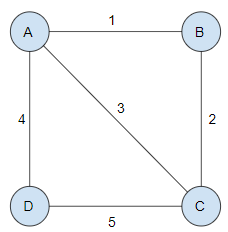
\includegraphics[scale=0.6]{assets/mst_1.png}
\end{center}
Consider the graph above. Find the minimum spanning tree. 

\begin{mdframed}[]
    From our lemma, we know that the edge of weight 1 must be in the tree since it is minimal. So, we can select it. 
    \begin{center}
        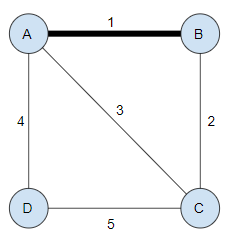
\includegraphics[scale=0.8]{assets/mst_2.png}
    \end{center}
    Our lemma doesn't say anything about what to do when we have to consider multiple edges. However, we can use a trick -- something we know is that $A$ and $B$ essentially form a connected component, so we can ``merge'' them together.
    \begin{center}
        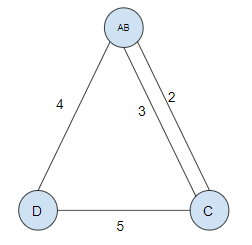
\includegraphics[scale=0.8]{assets/mst_2a.png}
    \end{center}
    From here, we can see that the edge of weight 2 must be in the tree since it is minimal. So, we can select it. 
    \begin{center}
        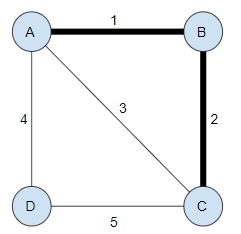
\includegraphics[scale=0.8]{assets/mst_3.png}
    \end{center}
    Making use of the same trick that we described above, we have: 
    \begin{center}
        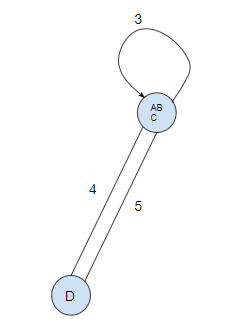
\includegraphics[scale=0.8]{assets/mst_3a.png}
    \end{center}
    Since MSTs cannot include loops, the edge of weight 4 must be in the tree since it is minimal. So, we can select it.
    \begin{center}
        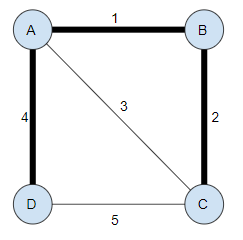
\includegraphics[scale=0.8]{assets/mst_4.png}
    \end{center}
    Since we have reached every vertex in $G$, we are done. Indeed, if we try to use the trick that we described above, we get: 
    \begin{center}
        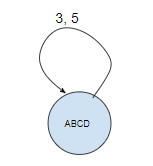
\includegraphics[scale=0.8]{assets/mst_4a.png}
    \end{center}
    Here, it's obvious that the only edges we need to consider would just loop back, and since we don't allow loops, we are done. 
\end{mdframed}
So, the lemma only gave us the first step of the process. However, by contracting along the edge, we get a new version of the original problem, from which we can apply the lemma again. By repeating this process, we get the MST. 

\subsubsection{Kruskal's Algorithm}
Kruskal's algorithm essentially says to repeatedly add the lightest edge that does not create a cycle. That is: 

\begin{verbatim}
    Kruskal(G):
        T = {}
        while |T| < |V| - 1:
            find lightest e such that T u {e} does not have a cycle 
            add e to T 

        return T 
\end{verbatim}
To check that $T \cup \{e\}$ doesn't create a cycle, we can check if the endpoints of $e$ are in different connected components of $T$. What we mean by this is, if we're just adding the lightest edge every time, it's possible that we'll have several trees; for the sake of simplicity, call these two trees $T_1$ and $T_2$. Then, if one endpoint of an edge $e$ is in $T_1$ and the other endpoint is in $T_2$, then it's not a cycle. If both endpoints $e$ are in $T_1$ or $T_2$ (but not both), then this will form a cycle and so we don't consider this $e$.

\bigskip 

The while loop runs in roughly $\BigO(|V|)$ time. For each iteration, we need to check if there is a cycle that can be formed by picking some $e$; this takes $\BigO(|V|)$ time. Going through all of the edges take $\BigO(|E|)$ time. Therefore, the final runtime is $\BigO(|V|^2 |E|)$ time. 

\subsubsection{First Optimization of Krustal's Algorithm: Recomputing Edge Weights}
Something to note is that, when we're checking edge weights, we're constantly going to see the same edges. If we, for example, add an edge $e = 5$ to our tree, then we don't need to consider the edges with weight less than 5. So, one optimization we can make is to simply not consider any edges that have weight less than the heaviest edge in the tree. So: 
\begin{verbatim}
    Kruskal(G):
        T = {}
        for e in E in increasing order of weight:
            if endpoints in different connected components:
                add e to T 
        return T 
\end{verbatim}
Sorting takes $\BigO(|E|\log(|E|))$. The loop goes through $|E|$ iterations, and computing the connected components takes $|V|$ time. So, our new runtime is 
\[\BigO(|E|\log(|E|) + |V||E|) = \BigO(|V||E|)\]
which is somewhat better. 

\subsubsection{First Optimization of Krustal's Algorithm: Union-Find}
Something else to note is that, when checking connected components, we're essentially computing the same connected components over and over again, all while barely making changes to said connected components. So, we want a data structure that can keep track of a bunch of sets. The idea is that we want a data structure that can
\begin{itemize}
    \item Create a new set: \code{v}
    \item Join two sets: \code{join(v, e)}
    \item Check representative element to see if $v$ and $w$ are in the same set: \code{rep(v)}
\end{itemize}
This is known as the \emph{union-find} data structure. Each set is a directed tree with the representative element at the root. This might look something like\footnote{Imagine each branch pointing upwards, and that each node can have more than 2 children (i.e. it's not a binary tree).}
\begin{verbatim}
                A
               / \ 
              /   \ 
             B     C 
            /|\     \ 
           / | \     \ 
          D  E  F     G 
\end{verbatim}
where the representative is $A$. So, creating a new set takes $\BigO(1)$ time. Finding the representative takes $\BigO(\text{depth of tree})$. Joining two trees (which is as simple as having one representative point to the other representative) takes $\BigO(\text{depth of tree})$ time, since we need to find the representative of the given elements. If we maintain the depth correctly, then the runtimes become $\BigO(\log(\text{number of nodes}))$. 

\bigskip 

So, with this in mind, our revised algorithm is as follows: 
\begin{verbatim}
    Kruskal(G):
        T = {}
        add each v to Union-Find data structure
        for e = (u, v) in increasing order of weight:
            if rep(u) != rep(v):
                add e to T 
                join(u, v)
        return T 
\end{verbatim}
Sorting takes $\BigO(|E|\log(|E|))$. Adding $|V|$ vertices take $\BigO(|V|)$ times ($|V|$ \code{join} calls). Then, iterating through each edge takes $\BigO(|E|)$ time. For each edge, we need to perform $|E|$ \code{rep} operations, and it we have $|V|$ \code{join} operations. Overall, this takes $\BigO(|E|\log(|E|))$ time, assuming we have a reasonable union-find implementation\footnote{Note that the above discussion of union-find is far from ideal. We can make use of, say, path compression to make this more ideal.}. 

\subsubsection{Trees and Cuts}
\begin{lemma}{}{}
    Let $G$ be a weighted graph, and let $C$ be a cut (i.e. a partition of the vertices of $G$ into two sets). 
    \begin{itemize}
        \item Let $e$ be a lowest weight edge crossing $C$. Then, there exists a MST of $G$ that contains $e$. 
        \item Let $e$ be the unique lowest weight edge crossing $C$. Then, every MST of $G$ contains $e$. 
    \end{itemize}
\end{lemma}

\begin{mdframed}[]
    \begin{proof}
        Suppose we have a cut $C$ which splits the vertices $V$ into two subsets $V_1$ and $V_2$. Let $T$ be a MST; then, $T$'s edges will have to cross this cut at some point. If $e \in T$, we're done. Otherwise, we can add the edge to $T$ such that it crosses the cut. This creates a cycle $R$, which implies that $R$ contains some other $e'$ that crosses the cut $C$. Then, let
        \[T' = T \cup \{e\} \setminus \{e'\}\]
        Then, the weight of $T'$ is given by 
        \[w(T') = w(T) + w(e) - w(e')\]
        but since $e$ is a minimum weight edge, and the weight of $e$ must be no more than $e'$, so it follows that 
        \[w(T') \leq w(T)\] 
        Additionally, if $e$ is a unique minimum weight edge, then $w(T') < w(T)$, which is a contradiction as this implies that $T$ wasn't a minimum spanning tree. So, we are done. 
    \end{proof}
\end{mdframed}

\subsubsection{Prim's Algorithm}
Prim's algorithm relies on the above lemma. Let $b(v)$ be the lightest weight edge (for vertices that we have not reached) that we have discovered that allows us to reach $v$ from the vertices that we have reached. 
\begin{verbatim}
    Prims(G):
        T = {}
        b(v) = inf 
        b(s) = 0
        Insert all V's into priority queue Q 
        while Q not empty:
            u = DeleteMin(Q)
            If u != s:
                Add (u, prev(u)) to T 
            For all (u, v) in E: 
                if v in Q and b(v) > l(u, v):
                    b(v) = l(u, v)
                    DecreaseKey(v)
                    prev(v) = u 
        return T 
\end{verbatim}
Basically, what's going on is that: 
\begin{itemize}
    \item For all $v$ in the priority queue (which we haven't reached), $b(v)$ will store the cheapest length of an edge that connects it to some vertex that is already connected to $s$, and \code{prev(v)} will tell you the other end of that best edge.
    \item So, find the vertex in $Q$ with the smallest with the smallest value of $b$, which is the lightest edge which connects some vertex in $u$ which has been connected to $s$ to some vertex that hasn't. We will add that edge to the tree, and then we need to do some updates. 
\end{itemize} 
This algorithm looks nearly like Dijkstra's algorithm, and in fact has the same runtime as Dijkstra's algorithm. That is, $\BigO(|V|\log(|V|) + |E|)$.





























\newpage 
\section{Dynamic Programming}
Consider the Fibonacci sequence 
\[F_n = F_{n - 1} + F_{n - 2}\]
The naive algorithm would just recursively call $F_{n - 1}$ and $F_{n - 2}$, which is very inefficient, especially since we would be making duplicate calls. Instead, we can \emph{tabulate} the answers, thus saving us a bunch of time. 

\bigskip 

So, what is a dynamic program? The idea is as follows: 
\begin{enumerate}
    \item Relate your answer to some family of similar subproblems. In the case of Fibonacci, we had to relate the $n$th Fibonacci number to all of the Fibonacci numbers before it; that is, we had to compute $F_t$ for all $t \in [t, n] \subseteq \Z$.
    \item There should be a recurrence relation that gives the answer to each subproblem in terms of answers to simpler subproblems. 
    \item Create a \emph{table}, compute the answers to all subproblems, and then tabulate them (store the answers in the table so that you can refer back to the table when you need the answer from the previous iteration for your current iteration). This is done in the simplest to most complicated order. 
\end{enumerate}
\textbf{Remark:} You can \emph{usually} look up entries in the table in constant time. Generally speaking, the table is done using an array or a hash map. 

\bigskip 

A few notes about dynamic programming. 
\begin{itemize}
    \item The general correct proof outline is to prove by induction that each table entry is filled out correctly. Essentially, you want to make sure the base case is correct, and then make use of the recurrence relationship for the inductive hypothesis.
    \item The runtime of dynamic programming is \emph{usually} the number of subproblems \emph{multiplied by} the time per subproblem. 
    \item For finding the recurrence, which is very important in a dynamic programming algorithm, you often look at the first or last choice and see what things look like without that choice.
\end{itemize}


\subsection{Problem: Longest Common Subsequence}
Given a sequence $a_1 a_2 \dots a_n$, we can get a subsequence by removing some entries in the sequence. For example, if we have a sequence \code{ABCD}, a subsequence would be \code{ACD} (by removing the \code{B}). Given two sequences $a_1 a_2 \dots a_n$ and $b_1 b_2 \dots b_m$, then the common subsequence is just some $c_1 \dots c_k$ that is a subsequence of both $a_1 a_2 \dots a_n$ and $b_1 b_2 \dots b_m$. 

\bigskip 

So, the problem statement is as follows: Given two sequences, compute the longest common subsequences. That is, the subsequence with as many letters as possible. 

\subsubsection{Example: Longest Common Subsequence}
Suppose $X = \code{ABCBA}$ and $Y = \code{ABACA}$. Then, the longest common subsequence of $X$ and $Y$ is \code{ABCA}.

\subsubsection{Case Analysis}
How do we compute \code{LCSS}($A_1 A_2 \dots A_n$, $B_1 B_2 \dots B_m$)? We need to consider several cases for the common subsequence. 
\begin{enumerate}
    \item It does not use $A_n$ (it does not use the last letter in the sequence $A$). That is, if the common subsequence does not use $A_n$, it is actually a common subsequence of 
    \[A_1 A_2 A_{n - 1} \text{ and } B_1 B_2 \dots B_m\]
    Therefore, in this case, the longest common subsequence would be 
    \[\code{LCSS}(A_1 A_2 \dots A_{n - 1}, B_1 B_2 \dots B_m)\]


    \item It does not use $B_m$ (It does not use the last letter in the sequence $B$). If the common subsequence does not use $B_m$, it is actually a common subsequence of 
    \[A_1 A_2 A_n \text{ and } B_1 B_2 \dots B_{m - 1}\]
    Therefore, in this case, the longest common subsequence would be 
    \[\code{LCSS}(A_1 A_2 \dots A_n, B_1 B_2 \dots B_{m - 1})\]

    
    \item It uses both $A_n$ and $B_m$, and these characters are the same. If a common subsequence uses both $A_n$ and $B_m$, then:
    \begin{itemize}
        \item These characters must be the same.
        \item Such a subsequence can be obtained by taking a common subsequence of $A_1 A_2 \dots A_{n - 1}$ and $B_1 B_2 \dots B_{m - 1}$ and adding a copy of $A_n = B_m$ to the end. 
        \item Therefore, the longest length of such a subsequence is given by 
        \[\code{LCSS}(A_1 A_2 \dots A_n, B_1 B_2 \dots B_{m - 1}) + 1\]
    \end{itemize}
\end{enumerate}
\textbf{Remark:} We can be in both case 1 and case 2.

\subsubsection{Recursion}
We've broken the longest common subsequence into three different cases, and for each of these cases we managed to compute the longest common subsequence of subsequences in that case by a longest common subsequence problem that is a little bit simpler than the one that we started at. Of course, the \emph{best} longest common subsequence overall is just the best that we can get from any of these three cases. 

\bigskip 

So, all we need to do is look at the three cases and take the \emph{maximum} of the subsequences. That is
\[\code{LCSS}(A_1 A_2 \dots A_n, B_1 B_2 \dots B_m) = \max \begin{rcases}
    \begin{dcases}
        \code{LCSS}(A_1 A_2 \dots A_{n - 1}, B_1 B_2 \dots B_m) \\ 
        \code{LCSS}(A_1 A_2 \dots A_n, B_1 B_2 \dots B_{m - 1}) \\ 
        \code{LCSS}(A_1 A_2 \dots A_{n - 1}, B_1 B_2 \dots B_{m - 1})
    \end{dcases}
\end{rcases}\]
where the last option is allowed only if $A_n = B_m$. 

\subsubsection{Analyzing Recursive Calls}
Suppose we make a call to \code{LCSS}($A_1 \dots A_n$, $B_1 \dots B_m$). What recursive calls are made? 
\begin{center}
    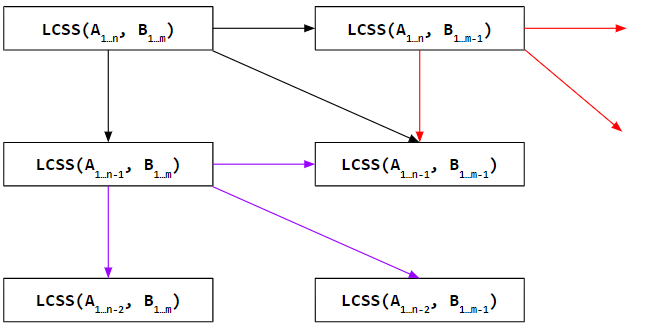
\includegraphics[scale=0.9]{assets/lcss_1.png}
\end{center}
Here, many recursive calls are omitted. However, the key thing to note is that we're making a call to \code(LCSS)($A_1 A_2 \dots A_{n - 1}$, $B_1 B_2 \dots B_{m - 1}$) three times (there are three different paths to get to that function call). 

\begin{note}{}{}
    This is the key difference between a dynamic programming algorithm and a divide and conquer algorithm. 
    \begin{itemize}
        \item The recursive subcalls for a divide and conquer algorithm are significantly smaller than the original problem. So, you never have to compute that many recursive subcalls even if you do the entire recursion tree.
        \item The recursive subcalls for a dynamic program algorithm are almost as big as the original call. \emph{However}, the same subproblems will show up multiple times in the recursion tree. So, rather than recomputing each subproblem, we can compute each subproblem once and then \emph{store} the result so we can refer to it later if we need it. 
    \end{itemize}
    In the case of our problem above, we only ever see $\code{LCSS}(A_1 A_2 \dots A_k, B_1 B_2 \dots B_{\ell})$ for some $k$ and $\ell$. 
\end{note}

\subsubsection{Base Case}
Our recursion also needs a base case. So, our base case is: 
\[\code{LCSS}(\emptyset, B_1 B_2 \dots B_m) = \code{LCSS}(A_1 A_2 \dots A_n, \emptyset) = 0\]

\subsubsection{Algorithm}
To take advantage of the fact that our dynamic program makes multiple \emph{repeated} subcalls (i.e. subcalls with the same inputs), we use \emph{tabulation} to \emph{store} the results of one subcall and then, when needed, we can retrieve the results of the subcall. 

\bigskip 

Thus, our algorithm is\footnote{Because the \code{verbatim} environment is limiting, I'll represent $A_1 A_2 \dots A_n$ as $A[1..n]$ and $B_1 B_2 \dots B_m$ as $B[1..m]$.}: 
\begin{verbatim}
    LCSS(A[1..n], B[1..m]):
        Initialize Array T[0..n, 0..m]
        // T[i, j] will store LCSS(A[1..i, 1..j])
        For i = 0 to n: 
            For j = 0 to m:
                // Base Case 
                If i == 0 OR j == 0: 
                    T[i, j] = 0
                
                // Case (3)
                Else if A[i] == B[j]
                    T[i, j] = max(T[i - 1, j], T[i, j - 1], T[i - 1, j - 1] + 1)
                
                // Case (1) or (2)
                Else: 
                    T[i, j] = max(T[i - 1, j], T[i, j - 1])

        Return T[n, m]
\end{verbatim}
The runtime is as follows: 
\begin{itemize}
    \item The outer loop runs in $n$ time. 
    \item The inner loop runs in $m$ time. 
    \item Everything inside the inner loop runs in constant time. 
\end{itemize}
This gives us the runtime $\BigO(nm)$. 

\subsubsection{Example: Longest Common Subsequence Redux}
Suppose $X = \code{ABCBA}$ and $Y = \code{ABACA}$. Find the longest common subsequence.

\begin{mdframed}[]
    We will tabulate the process. Call the table $T$. 
    \begin{center}
        \begin{tabular}{|c|c|c|c|c|c|c|}
            \hline 
                & $\emptyset$ & \code{A} & \code{AB} & \code{ABA} & \code{ABAC} & \code{ABACA} \\
            \hline 
            $\emptyset$     &   &   &   &   &   & \\ 
            \hline
            \code{A}        &   &   &   &   &   & \\ 
            \hline
            \code{AB}       &   &   &   &   &   & \\ 
            \hline
            \code{ABC}      &   &   &   &   &   & \\ 
            \hline
            \code{ABCB}     &   &   &   &   &   & \\ 
            \hline
            \code{ABCBA}    &   &   &   &   &   & \\ 
            \hline
        \end{tabular}
    \end{center}

    We will go through each table one row at a time. 
    \begin{enumerate}
        \item If we start at \code{i = 0}, then regardless of the value of \code{j}, the entire first row will be \code{0} by the first \code{if}-condition. So: 
        \begin{center}
            \begin{tabular}{|c|c|c|c|c|c|c|}
                \hline 
                    & $\emptyset$ & \code{A} & \code{AB} & \code{ABA} & \code{ABAC} & \code{ABACA} \\
                \hline 
                $\emptyset$     & 0 & 0 & 0 & 0 & 0 & 0 \\ 
                \hline
                \code{A}        &   &   &   &   &   &   \\ 
                \hline
                \code{AB}       &   &   &   &   &   &   \\ 
                \hline
                \code{ABC}      &   &   &   &   &   &   \\ 
                \hline
                \code{ABCB}     &   &   &   &   &   &   \\ 
                \hline
                \code{ABCBA}    &   &   &   &   &   &   \\ 
                \hline
            \end{tabular}
        \end{center}

        \item Now, when \code{i = 1}, then we need to consider the value of \code{j}. 
        \begin{itemize}
            \item If \code{j = 0}, then the entry at \code{T[1, 0] = 0}.
            
            \item If \code{j = 1}, then we're comparing \code{A} with \code{A}, so we need to consider the second \code{if}-condition. In this case, we need to check the entry directly above (\code{T[i - 1, j]}), to the left (\code{T[i, j - 1]}), and directly adjacent in the top-left entry (\code{T[i - 1, j - 1] + 1}). Here, we see that the values are \code{0}, \code{0}, and \code{0 + 1 = 1}, respectively. So, we store the \emph{maximum} of these values in \code{T[1, 1]}. Thus, \code{T[1, 1] = 1}. 
            
            \item If \code{j = 2}, then we're comparing \code{A} with \code{AB}, so we need to consider the third \code{if}-condition. In this case, we check the entry directly above \code{T[i - 1, j]} and directly to the left (\code{T[i, j - 1]}), and take the maximum. In our case, we have \code{0} and \code{1} (which we computed from the previous bullet point), respectively. Thus, \code{T[1, 2] = 1}.
            
            \item If \code{j = 3}, then we're comparing \code{A} with \code{AB}, so we need to consider the second \code{if}-condition. In this case, we check the entry directly above, left, and adjacent (add one to the end result) of \code{[i, j] = [1, 3]}. We get the values \code{0}, \code{1}, and \code{0 + 1 = 1}, respectively. Thus, \code{T[1, 3] = 1}.  
            
            \item Continuing on, we get \code{1}'s for the remaining cells in this row. 
        \end{itemize}
        Therefore, the second row is: 
        \begin{center}
            \begin{tabular}{|c|c|c|c|c|c|c|}
                \hline 
                    & $\emptyset$ & \code{A} & \code{AB} & \code{ABA} & \code{ABAC} & \code{ABACA} \\
                \hline 
                $\emptyset$     & 0 & 0 & 0 & 0 & 0 & 0 \\ 
                \hline
                \code{A}        & 0 & 1 & 1 & 1 & 1 & 1 \\ 
                \hline
                \code{AB}       &   &   &   &   &   &   \\ 
                \hline
                \code{ABC}      &   &   &   &   &   &   \\ 
                \hline
                \code{ABCB}     &   &   &   &   &   &   \\ 
                \hline
                \code{ABCBA}    &   &   &   &   &   &   \\ 
                \hline
            \end{tabular}
        \end{center}

        Omitting the rest of the work, we see that the result is: 
        \begin{center}
            \begin{tabular}{|c|c|c|c|c|c|c|}
                \hline 
                    & $\emptyset$ & \code{A} & \code{AB} & \code{ABA} & \code{ABAC} & \code{ABACA} \\
                \hline 
                $\emptyset$     & 0 & 0 & 0 & 0 & 0 & 0 \\ 
                \hline
                \code{A}        & 0 & 1 & 1 & 1 & 1 & 1 \\ 
                \hline
                \code{AB}       & 0 & 1 & 2 & 2 & 2 & 2 \\ 
                \hline
                \code{ABC}      & 0 & 1 & 2 & 2 & 3 & 3 \\ 
                \hline
                \code{ABCB}     & 0 & 1 & 2 & 2 & 3 & 3 \\ 
                \hline
                \code{ABCBA}    & 0 & 1 & 2 & 3 & 3 & 4 \\ 
                \hline
            \end{tabular}
        \end{center}
        And so the answer is given by the bottom-right entry, or \boxed{\code{4}}. 
    \end{enumerate}
\end{mdframed}

\subsubsection{Finding the Longest Common Subsequence}
The above algorithm finds the \emph{length} of the longest common subsequence. What if we wanted the actual subsequence? Well, we can \emph{backtrack}. So, consider the table above. 
\begin{center}
    \begin{tabular}{|c|c|c|c|c|c|c|}
        \hline 
            & $\emptyset$ & \code{A} & \code{AB} & \code{ABA} & \code{ABAC} & \code{ABACA} \\
        \hline 
        $\emptyset$     & 0 & 0 & 0 & 0 & 0 & 0 \\ 
        \hline
        \code{A}        & 0 & 1 & 1 & 1 & 1 & 1 \\ 
        \hline
        \code{AB}       & 0 & 1 & 2 & 2 & 2 & 2 \\ 
        \hline
        \code{ABC}      & 0 & 1 & 2 & 2 & 3 & 3 \\ 
        \hline
        \code{ABCB}     & 0 & 1 & 2 & 2 & 3 & 3 \\ 
        \hline
        \code{ABCBA}    & 0 & 1 & 2 & 3 & 3 & 4 \\ 
        \hline
    \end{tabular}
\end{center}
We can use this trick, based on the recurrence, to find out what the subsequence is. If you're at \code{[i, j]}, consider the neighbors \code{[i - 1, j]}, \code{[i, j - 1]}, and \code{[i - 1, j - 1]}. 
\begin{itemize}
    \item If the values at all three of those entries are equal, then take the diagonal path; that is, take \code{[i - 1, j - 1]}.
    \item If \code{[i - 1, j - 1]} and \code{[i - 1, j]} are equal but \code{[i, j - 1]} isn't equal to any of those two, then take the \code{[i, j - 1]} path. 
    \item If \code{[i - 1, j - 1]} and \code{[i, j - 1]} are equal but \code{[i - 1, j]} isn't equal to any of those two, then take the \code{[i - 1, j]} path. 
\end{itemize}
Once you reach the beginning, then you backtrack again. For each \emph{diagonal} path that was taken, take the last letter of one of the subsequences (the subsequences corresponding to the cell should end with the same letter). Once you reach back to the bottom-right square, then you can just concatenate the letters that you found.
\begin{center}
    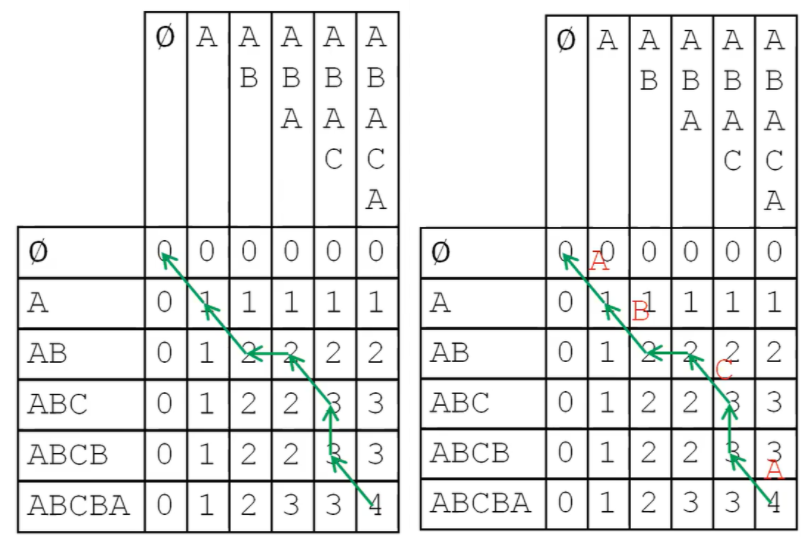
\includegraphics[scale=0.7]{assets/lcss_2.png}
\end{center}


\subsubsection{Proof of Correctness}
We now need to prove, by induction, that this algorithm is correct. 

\begin{mdframed}[]
    \begin{proof}
        We will use induction on $i$, $j$ to show that the value assigned to $T[i, j]$ is the correct value for \code{LCSS}($A_1 \dots A_i$, $B_1 \dots B_j$).
        \begin{itemize}
            \item \underline{Base Case:} When $i = 0 $ or $j = 0$, then we assign \code{0} since the empty string has no common subsequence with a string of some length. 
            \item \underline{Inductive Step:} Suppose the previous values are assigned correctly. We note that, because of the recursive relationship and the inductive hypothesis (since we have previously filled out $T[i - 1, j]$, $T[i, j - 1]$, and $T[i - 1, j - 1]$ correctly), that $T[i, j]$ gets the correct values. 
        \end{itemize}
        This completes the proof. 
    \end{proof}
\end{mdframed}

\subsection{Problem: Knapsack}
You are a burglar and are in the process of robbing a home. You have found several valuable items, but the sack you brought can only hold so much weight. What is the best combination of items to steal? 

\bigskip 

Some alternative formulations are: 
\begin{itemize}
    \item You are packing for a trip and your suitcase can only store so much stuff. You want to pack the most useful items for this trip. 
    \item You're building a spacecraft, but launching a spacecraft is incredibly expensive based on its weight. So, you want to decide what are the best modules to put on a spacecraft. 
\end{itemize}

\textbf{Problem Statement:} You have an available list of items. Each item has a non-negative integer weight. Your sack also has a capacity. The goal is to find the collection of items so that:
\begin{enumerate}
    \item The total weight of all of the items is less than or equal to the capacity.
    \item Subject to condition 1, the total value is as large as possible. 
\end{enumerate}
There are two slight variations of this problem:
\begin{itemize}
    \item Each item can be taken as many times as you want. 
    \item Each item can be taken at most once. 
\end{itemize}
In our case, we'll assume that you can take each item as many times as you want. 

\subsubsection{Example: Knapsack}
Suppose you have the following items: 
\begin{center}
    \begin{tabular}{c|c|c}
        \textbf{Item} & \textbf{Weight} & \textbf{Value} \\ 
        \hline 
        A & 1 & \$1 \\ 
        B & 2 & \$4 \\ 
        C & 3 & \$3 \\ 
        D & 4 & \$5
    \end{tabular}
\end{center}
Further suppose that the maximum capacity is 6. What is the best set of items to take, assuming you can only take one copy of each item? 

\begin{mdframed}[]
    We can brute-force this. 
    \begin{itemize}
        \item With weights $1 + 2 + 3 = 6$ (A, B, C), you can get $1 + 4 + 3 = \$8$. 
        \item With weights $4 + 2 = 6$ (B, D), you can get $5 + 4 = \$9$. 
    \end{itemize}
    The other weights smaller than 6 do not give us the best choice. Thus, the best set of items to take is $\{B, D\}$ with a value of \$9. 
\end{mdframed}


\subsubsection{Greedy Algorithms Don't Work}
Problems like this one usually suggest greedy algorithms as a solution. However, greedy algorithms don't work. To see that this is the case, consider the following two counterexamples.
\begin{enumerate}
    \item \underline{Most Valuable Item:} Suppose the greedy algorithm defines ``best'' to be the most valuable item. Suppose you have a knapsack of capacity 6 and the following set of items that you can steal, where you can only take one of each item. 
    \begin{center}
        \begin{tabular}{c|c|c}
            \textbf{Item} & \textbf{Weight} & \textbf{Value} \\ 
            \hline 
            A & 6 & \$10 \\ 
            B & 3 & \$9 \\ 
            C & 3 & \$9 
        \end{tabular}
    \end{center}
    Then: 
    \begin{itemize}
        \item The greedy solution would immediately go for $A$, since it is the most valuable item, which has value \textbf{\$10} and weight 6. 
        \item The optimal solution is $B$ and $C$, which has value \textbf{\$18} and weight 6.
    \end{itemize}

    \item \underline{Biggest Value/Weight:} Suppose the greedy algorithm defines ``best'' to be the item with the highest value to weight ratio. Again, suppose you have a knapsack of capacity 6 and the following set of items that you can steal, where you can only take one of each item. 
    \begin{center}
        \begin{tabular}{c|c|c}
            \textbf{Item} & \textbf{Weight} & \textbf{Value} \\ 
            \hline 
            A & 4 & \$5 \\ 
            B & 3 & \$3 \\ 
            C & 3 & \$3 
        \end{tabular}
    \end{center}
    Then:
    \begin{itemize}
        \item The greedy solution would immediately go for $A$, since $A$ has the highest value/weight ratio, which has value \textbf{\$5} and weight 4. Since the other items have weight 3 and $4 + 3 > 6$, we can't pick any of those items.  
        \item The optimal solution is $B$ and $C$, which has value \textbf{\$6} and weight 6.
    \end{itemize}
\end{enumerate}

\subsubsection{Subproblems}
Suppose we make \emph{one} choice of an item to go into the bag. Then, what is left? 
\begin{itemize}
    \item The remaining items must have a total weight at most $\text{Capacity} - \text{Weight of Item}$. 
    \item The total value of the items is 
    \[\text{Value of Item} + \text{Value of Other Items}\]
    \item Therefore, we want to maximize the value of the other items subject to their weight not exceeding the $\text{Capacity} - \text{Weight of Chosen Item}$.
\end{itemize}
Therefore, the subproblem is 
\[\text{BestValue}(\text{c'})\]
where $c'$ is the new capacity. 

\subsubsection{Recursion}
What is $\text{BestValue}(C)$, where $C$ is the capacity?
\begin{itemize}
    \item If there are \emph{no items} in the bag, then
    \[\text{Value} = 0\]
    \item If item $i$ is in the bag, then the value is given by 
    \[\text{Value} = \text{BestValue}(C - \text{Weight}(i)) + \text{Value}(i)\]
\end{itemize}
So, the best attainable value for a sack with capacity $C$ is the maximum of either: 
\begin{itemize}
    \item 0, \emph{or}
    \item For the item $i$ with weight such that $\text{Weight}(i) \leq C$ and $\text{Weight}(i)$ is maximal,
    \[\text{Value}(i) + \text{BestValue}(C - \text{Weight}(i))\]
\end{itemize}
Therefore, the recursion is given by 
\[\text{BestValue}(C) = \max(0, \max_{\text{Weight}(i) \leq C} \left(\text{Value}(i) + \text{BestValue}(C - \text{Weight}(i))\right))\]
Here, the 0 takes into account the possibility that the sack might be too small to fit any items. 

\subsubsection{Algorithm}
The algorithm, which makes use of the recurrence above, can be described like so: 
\begin{verbatim}
    Knapsack(Wt, Val, Cap):
        Create Array T[0..Cap]
        // Consider all capacities from 0..Cap 
        For C = 0 to Cap: 
            // Accounts for the fact that the sack might be too small to 
            // hold any items
            T[C] = 0
            // This is computing the maximum of all of the possible items
            For items i with Wt(i) <= C:
                If T[C] < Val(i) + T[C - Wt(i)]:
                    T[C] = Val(i) + T[C - Wt(i)]
        Return T[Cap]
\end{verbatim}
To see the runtime, we note that: 
\begin{itemize}
    \item There are $\BigO(\text{Cap})$ subproblems (the outer \code{for}-loop).
    \item For each subproblem, we need to (possibly) consider all of the possible items (the inner \code{for}-loop).
\end{itemize}
Therefore, the runtime is given by 
\[\BigO(\text{Cap} \cdot \text{Num. Items})\]

\subsubsection{Example: Knapsack Redux}
Suppose you have the following items: 
\begin{center}
    \begin{tabular}{c|c|c}
        \textbf{Item} & \textbf{Weight} & \textbf{Value} \\ 
        \hline 
        A & 1 & \$1 \\ 
        B & 2 & \$4 \\ 
        C & 3 & \$3 \\ 
        D & 4 & \$5
    \end{tabular}
\end{center}
Further suppose that the maximum capacity is 6. 

\begin{enumerate}
    \item What is the highest possible value you can get, (assuming you can only take as many of the same item as you want)? 

    \begin{mdframed}[]
        We can make use of the algorithm above. We define the table $T$ like so: 
        \begin{center}
            \begin{tabular}{|c|c|c|c|c|c|c|c|}
                \hline 
                \code{C}         & 0 & 1 & 2 & 3 & 4 & 5 & 6 \\ 
                \hline 
                \code{BestValue} &   &   &   &   &   &   &   \\ 
                \hline 
            \end{tabular}
        \end{center}
        \begin{itemize}
            \item Start at $c = 0$. Then, it's trivial to see that you can't get anything of value since, well, your capacity is 0. So, $T[0] = 0$ and 
            \begin{center}
                \begin{tabular}{|c|c|c|c|c|c|c|c|}
                    \hline 
                    \code{C}         & 0 & 1 & 2 & 3 & 4 & 5 & 6 \\ 
                    \hline 
                    \code{BestValue} & 0 &   &   &   &   &   &   \\ 
                    \hline 
                \end{tabular}
            \end{center}
    
            \item Now, we're at $c = 1$. By the algorithm we can initially set $T[1] = 0$. There are two choices that we can consider:
            \begin{itemize}
                \item We can fit item A in and get $\$1$.
                \item Or, we can fit nothing and get $\$0$.  
            \end{itemize}
            Clearly, the better choice is $\$1$, so we put that into $T[1]$. 
            \begin{center}
                \begin{tabular}{|c|c|c|c|c|c|c|c|}
                    \hline 
                    \code{C}         & 0 & 1 & 2 & 3 & 4 & 5 & 6 \\ 
                    \hline 
                    \code{BestValue} & 0 & 1 &   &   &   &   &   \\ 
                    \hline 
                \end{tabular}
            \end{center}
    
            \item Next, we're at $c = 2$. By the algorithm we can initially set $T[2] = 0$. There are several choices we can consider. 
            \begin{itemize}
                \item We can fit item B in and get $\$4$. 
                \item Or, we can take A, along with $T[1]$, and get $\$1 + \$1 = \$2$. 
            \end{itemize}
            Clearly, \$4 is the better choice, so we put that into $T[2]$. 
            \begin{center}
                \begin{tabular}{|c|c|c|c|c|c|c|c|}
                    \hline 
                    \code{C}         & 0 & 1 & 2 & 3 & 4 & 5 & 6 \\ 
                    \hline 
                    \code{BestValue} & 0 & 1 & 4 &   &   &   &   \\ 
                    \hline 
                \end{tabular}
            \end{center}
    
            \item Next, we're at $c = 3$. There are several choices to consider.
            \begin{itemize}
                \item We can fit item C in and get $\$3$.
                \item We can fit item A, along with what we already have in $T[2]$, and get $\$1 + \$4 = \$5$.
                \item We can fit item B, along with what we already have in $T[1]$, and get $\$2 + \$1 = \$3$. 
            \end{itemize}
            Clearly, \$5 is the better choice, so we put that into $T[3]$. 
            \begin{center}
                \begin{tabular}{|c|c|c|c|c|c|c|c|}
                    \hline 
                    \code{C}         & 0 & 1 & 2 & 3 & 4 & 5 & 6 \\ 
                    \hline 
                    \code{BestValue} & 0 & 1 & 4 & 5 &   &   &   \\ 
                    \hline 
                \end{tabular}
            \end{center}
    
            \item Next, we're at $c = 4$. There are, again, several cases to consider. 
            \begin{itemize}
                \item We can fit item D in and get $\$4$. 
                \item We can fit item C, along with what we have in $T[1]$, and get $\$3 + \$1 = \$4$.
                \item We can fit item B, along with what we have in $T[2]$, and get $\$4 + \$4 = \$8$. 
                \item We can fit item A, along with what we have in $T[3]$, and get $\$1 + \$5 = \$6$.
            \end{itemize}
            Here, we see that \$8 is the best choice, so we put that into $T[4]$. 
            \begin{center}
                \begin{tabular}{|c|c|c|c|c|c|c|c|}
                    \hline 
                    \code{C}         & 0 & 1 & 2 & 3 & 4 & 5 & 6 \\ 
                    \hline 
                    \code{BestValue} & 0 & 1 & 4 & 5 & 8 &   &   \\ 
                    \hline 
                \end{tabular}
            \end{center}
    
            \item Next, we're at $c = 5$. There are several choices to consider. 
            \begin{itemize}
                \item We can fit item D, along with $T[1]$, and get $\$5 + \$1 = \$6$.
                \item We can fit item C, along with $T[2]$, and get $\$3 + \$4 = \$7$.
                \item We can fit item B, along with $T[3]$, and get $\$4 + \$5 = \$9$.
                \item We can fit item A, along with $T[4]$, and get $\$1 + \$8 = \$9$.
            \end{itemize}
            Here, we see that \$9 is the best choice. So, we put that into $T[5]$. 
            \begin{center}
                \begin{tabular}{|c|c|c|c|c|c|c|c|}
                    \hline 
                    \code{C}         & 0 & 1 & 2 & 3 & 4 & 5 & 6 \\ 
                    \hline 
                    \code{BestValue} & 0 & 1 & 4 & 5 & 8 & 9 &   \\ 
                    \hline 
                \end{tabular}
            \end{center}
    
            \item Next, we're at $c = 6$. There are several choices to consider.
            \begin{itemize}
                \item We can fit item D, along with $T[2]$, and get $\$5 + \$4 = \$9$.
                \item We can fit item C, along with $T[3]$, and get $\$3 + \$5 = \$8$.
                \item We can fit item B, along with $T[4]$, and get $\$4 + \$8 = \$12$.
                \item We can fit item A, along with $T[5]$, and get $\$1 + \$9 = \$10$. 
            \end{itemize}
            Here, we see that \$12 is clearly the better choice. So, we put that in $T[6]$.
            \begin{center}
                \begin{tabular}{|c|c|c|c|c|c|c|c|}
                    \hline 
                    \code{C}         & 0 & 1 & 2 & 3 & 4 & 5 & 6 \\ 
                    \hline 
                    \code{BestValue} & 0 & 1 & 4 & 5 & 8 & 9 & 12 \\ 
                    \hline 
                \end{tabular}
            \end{center}
        \end{itemize}
        So, the answer is given by $T[6] = 12$. 
    \end{mdframed}

    \item What was the best possible set of items to collect? 
    \begin{mdframed}[]
        Remember that our table $T$ was populated to have the following values: 
        \begin{center}
            \begin{tabular}{|c|c|c|c|c|c|c|c|}
                \hline 
                \code{C}         & 0 & 1 & 2 & 3 & 4 & 5 & 6 \\ 
                \hline 
                \code{BestValue} & 0 & 1 & 4 & 5 & 8 & 9 & 12 \\ 
                \hline 
            \end{tabular}
        \end{center}
        So, we can backtrack to find out what items we collected. 
        \begin{itemize}
            \item First, we note that, to get \$12, we had to pick item B along with whatever was in $T[4]$. So, we know that \textbf{B} was an item that we collected. But, since we had to use whatever was in $T[4]$, we consider that entry next. 
            \item At $T[4] = 8$, we note that, to get $\$8$, we had to pick item B along with whatever was in $T[2]$. So, we know that \textbf{B} was an item that was collected. Additionally, since we had to use whatever was in $T[2]$, we consider that entry next. 
            \item At $T[2] = 4$, we note that, to get $\$4$, we had to pick item B. So, we know that \textbf{B} was an item that was collected. Since we didn't have to depend on the maximum value at some other entry, we're done. 
        \end{itemize}

        Therefore, we collected three \textbf{B}'s for a total of \textbf{\$12}. 
    \end{mdframed}
\end{enumerate}

\subsubsection{Non-Repeating Items: Subproblems}
Suppose we tried to do this process with non-repeating items. We can try to repeat what we did above (with the subproblems) for this case. That is, suppose we put one item into the bag. 
\begin{itemize}
    \item Then, the remaining items must have total weight at most $\text{Capacity} - \text{Weight of Item}$.
    \item The total value of the items is 
    \[\text{Value of Item} + \text{Value of Other Items}\]
    \item Therefore, we want to maximize the value of the other items subject to their weight not exceeding the $\text{Capacity} - \text{Weight of Chosen Item}$ \textbf{and} such that the chosen item(s) cannot be picked again. 
\end{itemize}
The recursion needs to now keep track of the remaining capacity, since the item that was picked cannotbe used again. This makes the problem a little harder. So, we can try to make several subproblems (where $c'$ is the new capacity).
\begin{enumerate}
    \item Suppose the subproblem we use is $\text{BestValue}_{\neq i}(c')$. In other words, the best value we can achieve without using item $i$ that doesn't go over the capacity. However, we \textbf{cannot} make a recursion out of this. This is because after using item $j$, the remaining items cannot include $i$ and $j$. However, we need to create a recursion such that a recursive subproblem can be solved in terms of other recursive subproblems.
    
    \item Suppose the subproblem we include is $\text{BestValue}_{\neq i, \neq j}(c')$. Again, we cannot make a recursion for this because this would imply the need to exclude a third item. 
    
    \item Suppose the subproblem we use is
    \[\text{BestValue}_{S}(c') = \max\left(0, \max_{i \in S}(\text{Value}(i) - \text{BestValue}_{S \setminus \{i\}}(\text{Cap} - \text{Weight}(i)))\right)\]
    In other words, the best value achievable using only items from $S$ with total weight at most $\text{Cap}$. This recursion \emph{works}, but this doesn't give us a very good algorithm. This is because the number of subproblems is more than $2^{\text{Number of Items}}$ since we're effectively considering every possible subset ($S \setminus \{i\}$). 
    
    \item Instead of trying the above approaches, let's think of something else. Suppose we have items coming along a conveyor belt. You decide, one at a time, whether to add the item to your sack. Then, the question we can think about is -- do we take the last item or leave it alone? 
    \begin{itemize}
        \item If we take the item, the recursion becomes
        \[\text{BestValue}_{\leq n - 1}(\text{Cap} - \text{Weight}(n)) + \text{Value}(n)\]
        \item If we don't take the item, then the recursion becomes 
        \[\text{BestValue}_{\leq n - 1}(\text{Cap})\]
    \end{itemize}
    If we tried to convert this into a recursion, then we only need subproblems of the form 
    \[\text{BestValue}_{\leq k}(\text{Cap})\]
    In other words, what happens to the first $k$ items? Somehow, by imposing this order, we don't need to deal with every possible subset of items.
\end{enumerate}

\subsubsection{Non-Repeating Items: Recursion}
So, our recursion $\text{BestValue}_{\leq k}(\text{Cap})$ is defined by the highest total value of items with the total weight at most \text{Cap} using only items from the first $k$. Thus:
\begin{itemize}
    \item \underline{Base Case:} If $k = 0$, then we can't take any items. So: 
    \[\text{BestValue}_{\leq 0}(\text{Cap}) = 0\]

    \item \underline{Recursion:} $\text{BestValue}_{\leq k}(\text{Cap})$ is the maximum of either: 
    \begin{enumerate}
        \item $\text{BestValue}_{\leq k - 1}(\text{Cap})$: You don't take the item, so we're finding the best value of the $k - 1$ items. 
        \item If $\text{Weight}(k) \leq \text{Cap}$, then $\text{BestValue}_{\leq k - 1}(\text{Cap} - \text{Weight}(k)) + \text{Value}(k)$: You take the item, add on the value, and then add on the best value of the $k - 1$ items. 
    \end{enumerate}
\end{itemize}

\subsubsection{Non-Repeating Items: Example}
Suppose you have the following items: 
\begin{center}
    \begin{tabular}{c|c|c}
        \textbf{Item} & \textbf{Weight} & \textbf{Value} \\ 
        \hline 
        A & 1 & \$1 \\ 
        B & 2 & \$4 \\ 
        C & 3 & \$3 \\ 
        D & 4 & \$5
    \end{tabular}
\end{center}
Further suppose that the maximum capacity is 6. 

\begin{enumerate}
    \item Find the highest possible value you can get, assuming you can only take one copy of each item. 

    \begin{mdframed}[]
        Instead of a one-dimensional table, we have a two-dimensional table $T$. 
        \begin{center}
            \begin{tabular}{|c|c|c|c|c|c|c|c|}
                \hline 
                \code{Cap}  & 0 & 1 & 2 & 3 & 4 & 5 & 6 \\ 
                \hline 
                $\emptyset$ &   &   &   &   &   &   &    \\ 
                \hline 
                \code{A}    &   &   &   &   &   &   &    \\ 
                \hline 
                \code{AB}   &   &   &   &   &   &   &    \\ 
                \hline 
                \code{ABC}  &   &   &   &   &   &   &    \\
                \hline 
                \code{ABCD} &   &   &   &   &   &   &    \\ 
                \hline 
            \end{tabular}
        \end{center}
        Here, we say that $T[\code{x}, n]$ refers to the cell with the row being \code{x} (the items that we can pick) and the column being $n$ (the capacity).
        \begin{itemize}
            \item At the row with the $\emptyset$, we essentially have $k = 0$. In other words, we're not able to pick anything. So, it follows that, regardless of capacity, if there's nothing to pick, we'll end up with $\$0$.
            \begin{center}
                \begin{tabular}{|c|c|c|c|c|c|c|c|}
                    \hline 
                    \code{Cap}  & 0 & 1 & 2 & 3 & 4 & 5 & 6 \\ 
                    \hline 
                    $\emptyset$ & 0 & 0 & 0 & 0 & 0 & 0 & 0  \\ 
                    \hline 
                    \code{A}    &   &   &   &   &   &   &    \\ 
                    \hline 
                    \code{AB}   &   &   &   &   &   &   &    \\ 
                    \hline 
                    \code{ABC}  &   &   &   &   &   &   &    \\
                    \hline 
                    \code{ABCD} &   &   &   &   &   &   &    \\ 
                    \hline 
                \end{tabular}
            \end{center}
    
            \item Suppose we're at the row with \code{A}; that is, we have $k = 1$ so we can pick one item, which in our case is $A$. Now, when the capacity is 0, clearly we cannot pick anything. But, as long as the capacity is greater than or equal to 1, we can pick A (value of 1). So: 
            \begin{center}
                \begin{tabular}{|c|c|c|c|c|c|c|c|}
                    \hline 
                    \code{Cap}  & 0 & 1 & 2 & 3 & 4 & 5 & 6 \\ 
                    \hline 
                    $\emptyset$ & 0 & 0 & 0 & 0 & 0 & 0 & 0  \\ 
                    \hline 
                    \code{A}    & 0 & 1 & 1 & 1 & 1 & 1 & 1  \\ 
                    \hline 
                    \code{AB}   &   &   &   &   &   &   &    \\ 
                    \hline 
                    \code{ABC}  &   &   &   &   &   &   &    \\
                    \hline 
                    \code{ABCD} &   &   &   &   &   &   &    \\ 
                    \hline 
                \end{tabular}
            \end{center}
    
            \item Suppose we're at the row with \code{AB}; that is, we're at $k = 2$ so we can pick two items, which in our case is $A$ or $B$. Now, when the capacity is 0, clearly we cannot pick anything. When the capacity is 1, clearly we can only pick $A$, so we can take $T[\code{A}, 1]$. When the capacity is 2, clearly the most optimal choice is $B$ (value of 4). When the capacity is greater than 2, we can pick $B$ and $T[\code{A}, c]$, where $c$ is the capacity such that $c > 2$ (value of 5).
            \begin{center}
                \begin{tabular}{|c|c|c|c|c|c|c|c|}
                    \hline 
                    \code{Cap}  & 0 & 1 & 2 & 3 & 4 & 5 & 6 \\ 
                    \hline 
                    $\emptyset$ & 0 & 0 & 0 & 0 & 0 & 0 & 0  \\ 
                    \hline 
                    \code{A}    & 0 & 1 & 1 & 1 & 1 & 1 & 1  \\ 
                    \hline 
                    \code{AB}   & 0 & 1 & 4 & 5 & 5 & 5 & 5  \\ 
                    \hline 
                    \code{ABC}  &   &   &   &   &   &   &    \\
                    \hline 
                    \code{ABCD} &   &   &   &   &   &   &    \\ 
                    \hline 
                \end{tabular}
            \end{center}
    
            \item Suppose we're at the row with \code{ABC}; that is, we're at $k = 3$ so we can pick three items, which in our case is $A$ or $B$ or $C$. 
            \begin{itemize}
                \item Now, when the capacity is 0, clearly we cannot pick anything. 
                
                \item When the capacity is 1, clearly we can pick $T[\code{AB}, 1]$ (value of 1). 
                
                \item When the capacity is 2, clearly the most optimal choice is $T[\code{AB}, 2]$ (value of 4). This is because there isn't any space for item $C$. 
                
                \item When the capacity is 3, clearly the most optimal choice is just $T[\code{AB}, 3]$. Note that if we picked $C$, then we would be worse-off. 
                
                \item When the capacity is 4, clearly the most optimal choice is just $T[\code{AB}, 4]$. Note that if we picked $C$, then we would be worse-off. 
                
                \item When the capacity is 5, we can pick $C$ and also $T[\code{AB}, 2]$ (value of 7). 
                
                \item When the capacity is 6, we can pick $C$ and also $T[\code{AB}, 3]$ (value of 8). 
            \end{itemize}
            Thus: 
            \begin{center}
                \begin{tabular}{|c|c|c|c|c|c|c|c|}
                    \hline 
                    \code{Cap}  & 0 & 1 & 2 & 3 & 4 & 5 & 6 \\ 
                    \hline 
                    $\emptyset$ & 0 & 0 & 0 & 0 & 0 & 0 & 0  \\ 
                    \hline 
                    \code{A}    & 0 & 1 & 1 & 1 & 1 & 1 & 1  \\ 
                    \hline 
                    \code{AB}   & 0 & 1 & 4 & 5 & 5 & 5 & 5  \\ 
                    \hline 
                    \code{ABC}  & 0 & 1 & 4 & 5 & 5 & 7 & 8  \\
                    \hline 
                    \code{ABCD} &   &   &   &   &   &   &    \\ 
                    \hline 
                \end{tabular}
            \end{center}
    
            \item Suppose we're at the row with \code{ABCD}; that is, we're at $k = 4$ so we can pick all four items if we can, which in our case is $A$ or $B$ or $C$ or $D$. 
            \begin{itemize}
                \item Now, when the capacity is 0, clearly we cannot pick anything. 
                
                \item When the capacity is 1, clearly we can pick $T[\code{ABC}, 1]$ (value of 1). 
                
                \item When the capacity is 2, clearly the most optimal choice is $T[\code{ABC}, 2]$ (value of 4). 
                
                \item When the capacity is 3, clearly the most optimal choice is just $T[\code{ABC}, 3]$. 
                
                \item When the capacity is 4, clearly the most optimal choice is just $T[\code{ABC}, 4]$. Here, we could also just pick $D$.
                
                \item When the capacity is 5, the optimal choice is just $T[\code{ABC}, 3]$ (value of 7). Note that the other option is $D$ and $A$, which is worse. 
                
                \item When the capacity is 6, we can pick $D$ and also $T[\code{ABC}, 2]$ (value of 9). 
            \end{itemize}
            Thus: 
            \begin{center}
                \begin{tabular}{|c|c|c|c|c|c|c|c|}
                    \hline 
                    \code{Cap}  & 0 & 1 & 2 & 3 & 4 & 5 & 6 \\ 
                    \hline 
                    $\emptyset$ & 0 & 0 & 0 & 0 & 0 & 0 & 0  \\ 
                    \hline 
                    \code{A}    & 0 & 1 & 1 & 1 & 1 & 1 & 1  \\ 
                    \hline 
                    \code{AB}   & 0 & 1 & 4 & 5 & 5 & 5 & 5  \\ 
                    \hline 
                    \code{ABC}  & 0 & 1 & 4 & 5 & 5 & 7 & 8  \\
                    \hline 
                    \code{ABCD} & 0 & 1 & 4 & 5 & 5 & 7 & 9  \\ 
                    \hline 
                \end{tabular}
            \end{center}
        \end{itemize}
        Thus, the final answer is given by $T[\code{ABCD}, 6] = 9$.
    \end{mdframed}

    \item Find the items that you took to get the maximum value found in the previous part. 
    
    \begin{mdframed}[]
        Using the table $T$ from the previous part: 
        \begin{center}
            \begin{tabular}{|c|c|c|c|c|c|c|c|}
                \hline 
                \code{Cap}  & 0 & 1 & 2 & 3 & 4 & 5 & 6 \\ 
                \hline 
                $\emptyset$ & 0 & 0 & 0 & 0 & 0 & 0 & 0  \\ 
                \hline 
                \code{A}    & 0 & 1 & 1 & 1 & 1 & 1 & 1  \\ 
                \hline 
                \code{AB}   & 0 & 1 & 4 & 5 & 5 & 5 & 5  \\ 
                \hline 
                \code{ABC}  & 0 & 1 & 4 & 5 & 5 & 7 & 8  \\
                \hline 
                \code{ABCD} & 0 & 1 & 4 & 5 & 5 & 7 & 9  \\ 
                \hline 
            \end{tabular}
        \end{center}
        We can backtrack to find out what items we collected. 
        \begin{itemize}
            \item Starting at $T[\code{ABCD}, 6]$, note that, in order to get to this position, we picked $T[\code{ABC}, 2]$ and $D$. So, we know that \textbf{D} was an item that we collected, and we additionally consider $T[\code{ABC}, 4]$. 
            \item Now that we're at $T[\code{ABC}, 2]$, note that, in order to get to this position, we picked $T[\code{AB}, 2]$. As we didn't pick up any other items along th way, we can just consider $T[\code{AB}, 2]$. 
            \item Now that we're at $T[\code{AB}, 2]$, note that, in order to get to this position, we picked \textbf{B}. Since we didn't consider any other entries in the table, we're done. 
        \end{itemize}
        Thus, the solution is \textbf{B} and \textbf{D}. 
    \end{mdframed}
\end{enumerate}

\subsection{Problem: Chain Matrix Multiplication}
How long does it take to multiply matrices? Suppose $A$ is an $n \times m$ matrix and $B$ is a $m \times k$ matrix. Then, for each entry of $C$ (which is a $n \times k$ matrix), of which there are $nk$ entries, we need to sum $m$ terms. Therefore, the runtime\footnote{We'll ignore Strassen's algorithm for the time being.} is just 
\[\BigO(nmk)\]
Suppose, now, we want to multiply three matrices $ABC$. We can multiply it two different ways since matrix multiplication is associative. That is, we can do it either way: 
\[A(BC) \qquad (AB)C\]
How long does it take to multiply each? Suppose $A$ is a $2 \times 3$ matrix, $B$ is a $3 \times 3$ matrix, and $C$ is a $3 \times 1$ matrix. 
\begin{itemize}
    \item If we did $A(BC)$, then multiplying $BC$ would take $3 \cdot 3 \cdot 1 = 9$ operations and multiplying $A(BC)$ would take $2 \cdot 3 \cdot 1 = 6$ operations. The total runtime is $9 + 6 = 15$. 
    \item If we did $(AB)C$, then multiplying $AB$ would take $2 \cdot 3 \cdot 3 = 18$ operations and multiplying $(AB)C$ would take $2 \cdot 3 \cdot 1 = 6$ operations. The total runtime is $18 + 6 = 24$. 
\end{itemize}
The point is, from this simple example, if the matrices are complicated (not square), the order that you multiply the matrices may matter a lot. 

\bigskip 

\textbf{Problem Statement:} Find the order to multiply the matrices $A_1, A_2, \dots, A_m$ that requires the fewest total operations. In particular, assume $A_1$ is an $n_0 \times n_1$ matrix, $A_2$ is an $n_1 \times n_2$ matrix, and generally $A_k$ is an $n_{k - 1} \times n_k$ matrix. 

\subsubsection{Recursion}
In order to find some sort of a recursion so we can make a dynamic programming algorithm, we can again consider the last step. For some value of $k$, the last step is: 
\[(\underbrace{A_1 A_2 \dots A_k}_{M_1}) (\underbrace{A_{k + 1} A_{k + 2} \dots A_m}_{M_2})\]
That is, we've already computed the product of $M_1$ and $M_2$, so the last step is to multiply $M_1$ and $M_2$. So, if we want to compute the big product of matrices, what's the best runtime? The number of steps is as follows: 
\begin{itemize}
    \item We first need to compute the first half; that is, $\code{CMM}(A_1, A_2, \dots, A_k)$. 
    \item We next need to compute the second half; that is, $\code{CMM}(A_{k + 1}, A_{k + 2}, \dots, A_m)$. 
    \item Finally, we need to do the final multiplication ($M_1 M_2$), which takes $n_0 n_k n_m$ operations. 
\end{itemize}
Therefore, the recursion $\code{CMM}(A_1, A_2, \dots, A_m)$ is given by 
\[\min_{k}\left(\code{CMM}(A_1, \dots, A_k) + \code{CMM}(A_{k + 1}, \dots, A_m) + n_0 n_k n_m\right)\]
Where we need to consider all possible chain matrix multiplication orders (so we need to take the minimum of all possible values of $k$). 

\subsubsection{Subproblems}
What subproblems do we need to solve? 
\begin{itemize}
    \item Remember, we cannot afford to solve all possible chain matrix multiplication problems. So, in other words, while we \emph{do} have a recursion, if we were to try every possible $k$, that would simply take too much time on its own. 
    \item We know that $\code{CMM}(A_1, \dots, A_k)$ requires $\code{CMM}(A_1, \dots, A_k)$ and $\code{CMM}(A_{k + 1}, \dots, A_m)$ for various values of $k$.
    \item Suppose we wanted to compute $\code{CMM}(A_1, \dots, A_k)$. We might need to break this down into pieces; some of those pieces will be $\code{CMM}(A_1, \dots, A_{k'})$ ($k' < k$) and some of the pieces will be $\code{CMM}(A_{k'}, \dots, A_k)$; these are all new subproblems to deal with. When we break \emph{these} down, we don't really get anything new; that is, if we tried to run $\code{CMM}(A_i, A_{i + 1}, \dots, A_{j})$ and break these into two halves, we still have consecutive intervals of these matrices. 
    \item So, the general recursive subproblem that we need to solve is of this form
    \[C(i, j) = \code{CMM}(A_i, A_{i + 1}, \dots, A_{j})\]
    for $1 \leq i \leq j \leq m$; so there are fewer than $m^2$ total subproblems. Essentially, all we're doing is We're taking some consecutive collection of indices and we want to compute the chain matrix multiplication of that. 
\end{itemize}

\subsubsection{Full Recursion}
We now talk about the components of this recursion. 
\begin{itemize}
    \item \underline{Base Case:} For the base case, $C(i, i) = 0$. All this is saying is that you want to multiply the matrix $A_i$ and that's it; so, there's only one matrix. With a single matrix, we don't need to do anything.
    \item \underline{Recursive Step:} The recursive step is given by 
    \[C(i, j) = \min_{i \leq k < j} \left(C(i, k) + C(k + 1, j) + n_i n_k n_j\right)\]
    If we have $i < j$, then $C(i, j)$ should be the \emph{minimum} of all possible places we can break this product into two pieces; in other words, it's the minimum of the two recursive calls plus the final computation. 
    \item \underline{Solution Order:} We need to solve the subproblems with smaller $j - i$ first. This ensures that the recursive calls will always be in your table.   
\end{itemize}

\subsubsection{Example: Chain Matrix Multiplication}
Suppose $A$ is a $2 \times 5$ matrix, $B$ is a $5 \times 4$ matrix, $C$ is a $4 \times 3$ matrix, and $D$ is a $3 \times 5$ matrix. 

\begin{enumerate}
    \item Compute the minimum number of operations needed to evaluate $ABCD$. 

    \begin{mdframed}[]
        We can build this table $T$: 
        \begin{center}
            \begin{tabular}{|c|c|c|c|c|}
                \hline
                         & \code{A} & \code{B} & \code{C} & \code{D} \\ 
                \hline 
                \code{A} &          &          &          &          \\
                \hline  
                \code{B} &          &          &          &          \\
                \hline 
                \code{C} &          &          &          &          \\
                \hline 
                \code{D} &          &          &          &          \\
                \hline      
            \end{tabular}
        \end{center}
        Here, we're performing chained matrix multiplication, where we start at some matrix (denoted by the row) and finish at another matrix (denoted by the column). So, if we chose the row $A$ and the column $C$, this means $ABC$. Thus, $T[X, Y]$ means that we start at matrix $X$ and end at matrix $Y$. Thus, we're interested in finding the value of $T[A, D]$ since this means the number of steps needed to compute $ABCD$. 
    
        \begin{itemize}
            \item First, we note that the bottom-left diagonal calls make no sense. For example, we don't need $T[C, B]$ as this is saying the number of operations needed to compute $CB$, but we will never need a subproblem where this is the case. So: 
            \begin{center}
                \begin{tabular}{|c|c|c|c|c|}
                    \hline
                             & \code{A} & \code{B} & \code{C} & \code{D} \\ 
                    \hline 
                    \code{A} &          &          &          &          \\
                    \hline  
                    \code{B} & \code{X} &          &          &          \\
                    \hline 
                    \code{C} & \code{X} & \code{X} &          &          \\
                    \hline 
                    \code{D} & \code{X} & \code{X} & \code{X} &          \\
                    \hline      
                \end{tabular}
            \end{center}
    
            \item Next, we start with the base case. That is, $T[A, A] = T[B, B] = T[C, C] = T[D, D] = 0$. So: 
            \begin{center}
                \begin{tabular}{|c|c|c|c|c|}
                    \hline
                             & \code{A} & \code{B} & \code{C} & \code{D} \\ 
                    \hline 
                    \code{A} &    0     &          &          &          \\
                    \hline  
                    \code{B} & \code{X} &    0     &          &          \\
                    \hline 
                    \code{C} & \code{X} & \code{X} &    0     &          \\
                    \hline 
                    \code{D} & \code{X} & \code{X} & \code{X} &    0     \\
                    \hline      
                \end{tabular}
            \end{center}
    
            \item Next, we look at $T[A, B]$. Recall that $A$ is a $2 \times 5$ matrix and $B$ is a $5 \times 4$ matrix. Further, there is only \emph{one} way to break down $AB$: as itself. So it follows that $AB$ will take $2 \cdot 5 \cdot 4 = 40$ operations to compute. 
            \begin{center}
                \begin{tabular}{|c|c|c|c|c|}
                    \hline
                             & \code{A} & \code{B} & \code{C} & \code{D} \\ 
                    \hline 
                    \code{A} &    0     &    40    &          &          \\
                    \hline  
                    \code{B} & \code{X} &    0     &          &          \\
                    \hline 
                    \code{C} & \code{X} & \code{X} &    0     &          \\
                    \hline 
                    \code{D} & \code{X} & \code{X} & \code{X} &    0     \\
                    \hline      
                \end{tabular}
            \end{center}
    
            \item Next, we look at $T[B, C]$. Again, there's only one way to break this down -- as itself. So, it follows that $BC$ will take $5 \cdot 4 \cdot 3 = 60$ operations to compute. 
            \begin{center}
                \begin{tabular}{|c|c|c|c|c|}
                    \hline
                             & \code{A} & \code{B} & \code{C} & \code{D} \\ 
                    \hline 
                    \code{A} &    0     &    40    &          &          \\
                    \hline  
                    \code{B} & \code{X} &    0     &    60    &          \\
                    \hline 
                    \code{C} & \code{X} & \code{X} &    0     &          \\
                    \hline 
                    \code{D} & \code{X} & \code{X} & \code{X} &    0     \\
                    \hline      
                \end{tabular}
            \end{center}
    
            \item For the same reason as above, $T[C, D]$ will take $4 \cdot 3 \cdot 5 = 60$ operations to compute. 
            \begin{center}
                \begin{tabular}{|c|c|c|c|c|}
                    \hline
                             & \code{A} & \code{B} & \code{C} & \code{D} \\ 
                    \hline 
                    \code{A} &    0     &    40    &          &          \\
                    \hline  
                    \code{B} & \code{X} &    0     &    60    &          \\
                    \hline 
                    \code{C} & \code{X} & \code{X} &    0     &    60    \\
                    \hline 
                    \code{D} & \code{X} & \code{X} & \code{X} &    0     \\
                    \hline      
                \end{tabular}
            \end{center}
    
            \item Next, we look at $T[A, C]$. Since there are three matrices here, there are two ways to break this down. 
            \begin{itemize}
                \item $A(BC)$: Note that $BC$ will be a $5 \times 3$ matrix. Since $A$ is a $2 \times 5$ matrix, it follows that 
                \[2 \cdot 5 \cdot 3 + T[B, C] = 30 + 60 = 90\]
                \item $(AB)C$: Note that $AB$ will be a $2 \times 4$ matrix. Since $C$ is a $4 \times 3$ matrix, it follows that 
                \[T[A, B] + 2 \cdot 4 \cdot 3 = 40 + 24 = 64\]
            \end{itemize}
            Taking the minimum of the total number of ways to break this problem down, we have \textbf{64}. So: 
            \begin{center}
                \begin{tabular}{|c|c|c|c|c|}
                    \hline
                             & \code{A} & \code{B} & \code{C} & \code{D} \\ 
                    \hline 
                    \code{A} &    0     &    40    &    64    &          \\
                    \hline  
                    \code{B} & \code{X} &    0     &    60    &          \\
                    \hline 
                    \code{C} & \code{X} & \code{X} &    0     &    60    \\
                    \hline 
                    \code{D} & \code{X} & \code{X} & \code{X} &    0     \\
                    \hline      
                \end{tabular}
            \end{center}
    
            \item Next, we look at $T[B, D]$. Since there are three matrices here, there are two ways to break this down as well. 
            \begin{itemize}
                \item $B(CD)$: Note that $CD$ is a $4 \times 5$ matrix. Since $B$ is a $5 \times 4$ matrix, it follows that 
                \[5 \cdot 4 \cdot 5 + T[C, D] = 100 + 60 = 160\]
                \item $(BC)D$: Note that $BC$ is a $5 \times 3$ matrix. Since $D$ is a $3 \times 5$ matrix, it follows that 
                \[T[B, C] + 5 \cdot 3 \cdot 5 = 60 + 75 = 135\]
            \end{itemize}
            Taking the minimum of the total number of ways to break this problem down, we have \textbf{135}. So: 
            \begin{center}
                \begin{tabular}{|c|c|c|c|c|}
                    \hline
                            & \code{A} & \code{B} & \code{C} & \code{D} \\ 
                    \hline 
                    \code{A} &    0     &    40    &    64    &          \\
                    \hline  
                    \code{B} & \code{X} &    0     &    60    &    135   \\
                    \hline 
                    \code{C} & \code{X} & \code{X} &    0     &    60    \\
                    \hline 
                    \code{D} & \code{X} & \code{X} & \code{X} &    0     \\
                    \hline      
                \end{tabular}
            \end{center}
    
            \item Finally, we look at $T[A, D]$. Since there are four matrices here, there are three ways to break this down. 
            \begin{itemize}
                \item $A(BCD)$: Here, we know that $T[B, D] = 135$. Additionally, since $BCD$ is a $5 \times 5$ matrix and $A$ is a $2 \times 5$ matrix, it follows that 
                \[2 \cdot 5 \cdot 5 + 135 = 185\]
                \item $(AB)(CD)$: Here, we know that $AB$ is a $2 \times 4$ matrix and $CD$ is a $4 \times 5$ matrix. Additionally, $T[A, B] = 40$ and $T[C, D] = 60$. So, it follows that 
                \[T[A, B] + 2 \cdot 4 \cdot 5 + T[C, D] = 40 + 40 + 60 = 140\]
                \item $(ABC)D$: Here, we know that $ABC$ is a $2 \times 3$ matrix and $D$ is a $3 \times 5$ matrix. Additionally, $T[A, C] = 64$. So, it follows that 
                \[T[A, C] + 2 \cdot 3 \cdot 5 = 64 + 30 = 94\]
            \end{itemize}
            Taking the minimum of the total number of ways to break this problem down, we have \textbf{94}. So: 
            \begin{center}
                \begin{tabular}{|c|c|c|c|c|}
                    \hline
                            & \code{A} & \code{B} & \code{C} & \code{D} \\ 
                    \hline 
                    \code{A} &    0     &    40    &    64    &    94    \\
                    \hline  
                    \code{B} & \code{X} &    0     &    60    &    135   \\
                    \hline 
                    \code{C} & \code{X} & \code{X} &    0     &    60    \\
                    \hline 
                    \code{D} & \code{X} & \code{X} & \code{X} &    0     \\
                    \hline      
                \end{tabular}
            \end{center}
        \end{itemize}
        Therefore, our solution is given by $T[A, D] = \textbf{94}$. 
    \end{mdframed}

    \item What order did you have to multiply the matrices to get the lowest possible of computations? 
    \begin{mdframed}[]
        We note that the least number of computations needed to evaluate $ABCD$ is given by 94. Like with the other examples, we can backtrack to figure out the order. 
        \begin{itemize}
            \item In order to get $T[A, D] = 94$, we had to compute $(ABC)D$. So, we need to go back to $T[A, C]$, which is 64. 
            \item Looking at $T[A, C] = 64$, we see that the we had to compute $(AB)C$. So, we need to go back to $T[A, B]$, which is 40.
            \item Looking at $T[A, B]$, there's only one way to multiply $AB$. So, we're done.  
        \end{itemize}
        From this, it follows that the order in which we multiplied these matrices is 
        \[ABCD \implies (ABC)D \implies \boxed{((AB)C)D}\]
    \end{mdframed}
    \textbf{Remark:} If we have a tie somewhere, this implies that there is more than one optimal solution. So, you can return one of the optimal solutions. 
\end{enumerate}

\subsubsection{Runtime}
The runtime of this algorithm is given by: 
\begin{itemize}
    \item \underline{Number of Subproblems:} We needed to index through all possible $(i, j)$ in the range $1 \leq i \leq j \leq m$. So, the total number of subproblems is at most $m^2$.
    \item \underline{Time per Subproblem:} We need to check each $i \leq k < j$ as one of your terms for the maximum. Each check takes constant time (two table lookups and some multiplication and additions). We need to check $m$ different values of $k$.
\end{itemize}
Thus, we have 
\[\BigO(m^2 m) = \BigO(m^3)\]

\subsubsection{Dynamic Programming Setup}
Sometimes, there are many ways to create a dynamic programming algorithm for a given problem. How we set it up will have a large effect on the runtime. 


\subsection{All Pairs Shortest Paths}
\textbf{Problem Statement:} Given a directed graph $G$ with possibly negative edge weights, compute the length of the shortest path between \underline{every pair} of vertices\footnote{Bellman-Ford computes the single-source shortest paths. Namely, for some fixed vertex $s$, it computes all of the shortest path lengths $d(s, v)$ for every $v$. In \emph{this} problem, we want to compute the shortest path from every vertex to every other vertex.}.

\subsubsection{Naive Algorithm}
The easy algorithm is to run Bellman Ford with source $s$ for each vertex $s$. The runtime is given by $\BigO(|V|^2 |E|)$. 

\subsubsection{Dynamic Program}
Let $d_{k}(u, v)$ be the length of the shortest path from $u$ to $v$ that uses at most $k$ edges. 
\begin{center}
    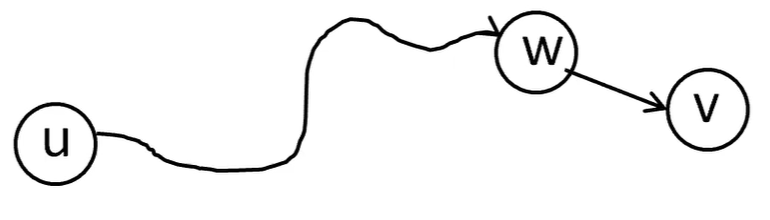
\includegraphics[scale=0.3]{assets/sp.png}
\end{center}
So, we can consider the last edge of that path; in our case, $w$ to $v$. Then, we have the path with length $k - 1$ from $u$ to $w$ followed by the edge $w$ to $v$. So: 
\[d_{k}(u, v) = \min_{w \in V}(d_{k - 1}(u, w) + \ell(w, v))\]

\subsubsection{Matrix Multiplication Method}
We know that Bellman Ford is slow in part because we can only increase $k$ by one step at a time. This happens because we cut off only the last edge of the optimal path. However, for computation distances from every vertex to every other vertex, there's a better way to do this. What if, instead, we cut this path in the middle in the middle instead of just one edge off of the end like we do with Bellman Ford?

\subsubsection{Recursion}
Suppose we have a path $u$ to $v$ with at most $2k$ edges: 
\begin{center}
    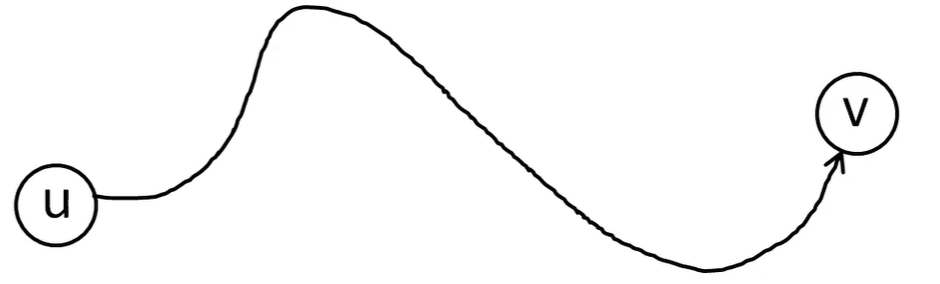
\includegraphics[scale=0.5]{assets/sp_2.png}
\end{center}
Then, we can always pick a vertex $w$ so that there are at most $k$ edges on either side of it, like so: 
\begin{center}
    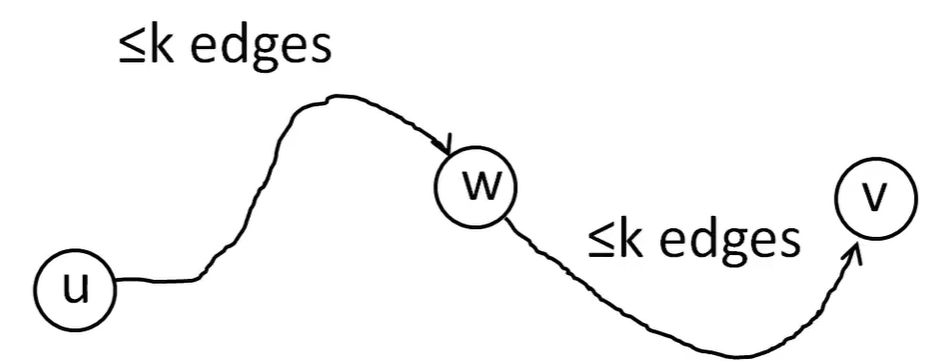
\includegraphics[scale=0.5]{assets/sp_3.png}
\end{center}
If we picked a particular vertex $w$, then the best length we will get is 
\[d_{2k}(u, v) = \min_{w \in V} (d_{k}(u, w) + d_{k}(w, v))\]
It's not hard to see that $d_{2k}(u, v)$ is just the minimum over all vertices $w$ that go in the middle. This gives us a somewhat different recurrence relation, and a totally different dynamic program for computing all pairs shortest path. 


\subsubsection{Algorithm}
How does the algorithm work? 

\begin{itemize}
    \item \underline{Base Case:} The base case is given by the path length if we only have 1 edge. 
    \[d_{1}(u, v) = \begin{cases}
        0 & \text{if } u = v \\ 
        \ell(u, v) & \text{if } (u, v) \in E \\ 
        \infty & \text{otherwise (no edge)} 
    \end{cases}\]

    \item \underline{Recursion:} Given $d_{k}(u, v)$ for all $u, v$, we can compute $d_{2k}(u, v)$ using 
    \[d_{2k}(u, v) = \min_{w \in V} (d_{k}(u, w) + d_{k}(w, v))\]

    \item \underline{End Condition:} We can compute $d_1, d_2, d_4, d_8, d_{16}, \dots, d_m$ until $m > |V|$. 
\end{itemize}

The base case takes $\BigO(|V|^2)$ time to fill the initial table. The recursion takes $\BigO(|V|^3)$; this is because we need to consider every pair, of which there are $|V|^2$ possibilities, and then taking the minimum of all third vertices. Finally, the end condition takes $\BigO(\log(|V|))$ time. Thus, the runtime is given by 
\[\BigO(|V|^3 \log(|V|))\]


\subsubsection{Floyd-Warshall Algorithm}
We can look at this problem in a different way. 
\begin{itemize}
    \item First, we \emph{label} the vertices $v_1, v_2, \dots, v_n$, where $n$ is the total number of vertices. 
    \item Next, we define $d_{k}(u, v)$ be the length of the shortest path from $u$ to $w$ using only $v_1, v_2, \dots, v_k$ as intermediate vertices. So, we are restricting what vertices we can use to get from one vertex to the other. 
\end{itemize}
Thus, the algorithm is given by: 
\begin{itemize}
    \item \underline{Base Case:} The base case is given by the fact that you aren't allowed to use any intermediate vertices. So: 
    \[d_{0}(u, v) = \begin{cases}
        0 & \text{if } u = v \\ 
        \ell(u, v) & \text{if } (u, v) \in E \\ 
        \infty & \text{otherwise (no edge)} 
    \end{cases}\]

    \item \underline{Recursion:} Suppose we want to get from $u$ to $w$ using only vertices $v_1, \dots, v_k$. We will consider several different cases depending on whether or not the shortest path uses $v_k$.
    \begin{itemize}
        \item If the shortest path does not use $v_k$, then it only uses the intermediate vertices $v_1, v_2, \dots, v_{k - 1}$. Thus, the shortest path is given by $d_{k - 1}(u, w)$. 
        \item If the shortest path does use $v_k$, then we can break this path down like so: 
        \begin{center}
            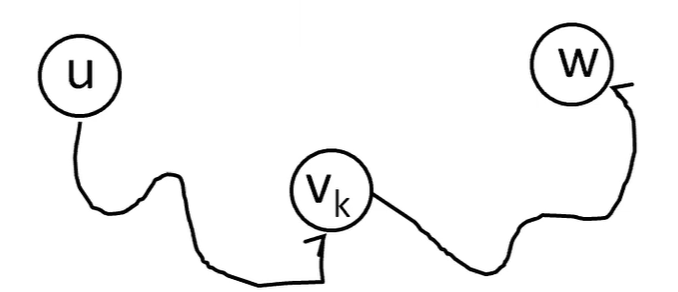
\includegraphics[scale=0.5]{assets/sp3.png}
        \end{center}
        It has length 
        \[d_{k - 1}(u, v_k) + d_{k - 1}(v_k, w)\]
        We can start at $u$, move through some intermediate vertices to get to $v_k$, and then move through more intermediate vertices to get to $w$. In either cases, the intermediate vertices can be $v_1$ to $v_{k - 1}$. 
    \end{itemize}
    In other words, for each $u$ and $w$, we want to compute 
    \[d_{k}(u, v) = \min(d_{k - 1}(u, w), d_{k - 1}(u, v_k) + d_{k - 1}(v_k, w))\]

    \item \underline{End Condition:} The end condition is given by 
    \[d(u, w) = d_{n}(u, w)\]
    where $n = |V|$. 
\end{itemize}
The runtime is given by 
\begin{itemize}
    \item The base case takes $\BigO(|V|^2)$ time to fill up the table. 
    \item The recursion takes $\BigO(|V|^2)$ time because there are $|V|^2$ pairs to consider.
    \item The end condition takes $\BigO(|V|)$ time. 
\end{itemize}
The final runtime is then 
\[\BigO(|V|^3)\]

\subsubsection{Best Known Algorithm}
The best known algorithm doesn't actually use dynamic programming. 
\begin{enumerate}
    \item Run Bellman-Ford \emph{once} to compute $d(v)$. 
    \item Then, we reweigh the edges. We replace the length $\ell$ with $\ell'$; $\ell'$ is given by (for every edge from $u$ to $w$)
    \[\ell'(u, w) = \ell(u, w) = d(u) - d(w) \geq 0\]
    There are two things to note: 
    \begin{itemize}
        \item $\ell'(u, w)$ will always be non-negative because $d(w) \leq d(u) + \ell(u, w)$. 
        \item Computing the shortest path with $\ell'(u, w)$ is equivalent to computing the shortest path with $\ell(u, w)$. 
    \end{itemize}
    
    \item Run Dijkstra's algorithm from every source. 
\end{enumerate}
The final runtime is given by 
\[\BigO(|V||E| + |V|^2 \log(|V|))\]

\subsection{Problem: Maximum Independent Set of Trees}

\begin{definition}{Independent Set}{}
    In an undirected graph $G$, an \textbf{independent set} is a subset of the vertices of $G$, no two of which are connected by an edge.
\end{definition}
For example, the following is an independent set:
\begin{center}
    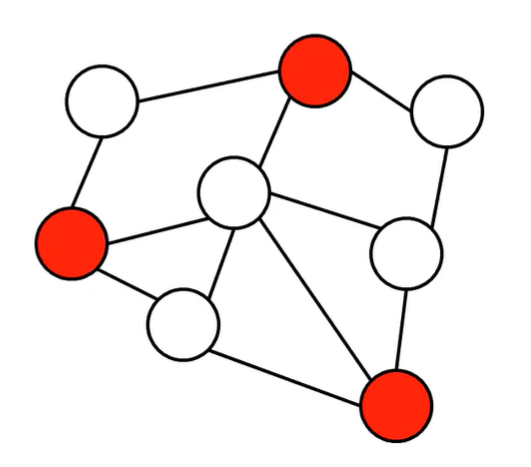
\includegraphics[scale=0.3]{assets/ind_set.png}
\end{center}

\textbf{Problem Statement:} Given an undirected graph $G$, compute the largest possible \textbf{size} of an independent set of $G$. 

\bigskip 

Call the result of the largest possible independent set $I(G)$; in the example above, $I(G) = 3$. 


\subsubsection{Simple Recursion}
\begin{center}
    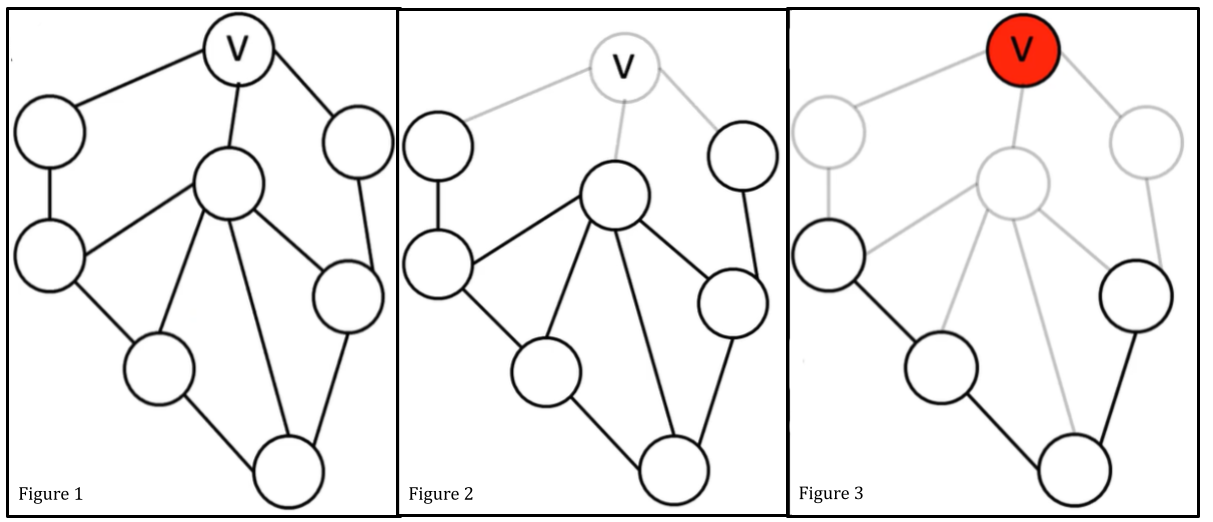
\includegraphics[scale=0.35]{assets/ind_set_ex.png}
\end{center}

There is a reasonably simple recursion that can be used here. A simple question we can ask is: \emph{is vertex $v$ in the independent set?} We'll consider Figure 1 above as a baseline example.
\begin{itemize}
    \item If $v$ is not in the independent set, then the maximum independent set is an independent set of $G \setminus \{v\}$. In other words, we have 
    \[I(G) = I(G \setminus \{v\})\]
    For example, Figure 2 shows what this could look like.
    \item If so, then the maximum independent set is $v$ plus an independent set of $G \setminus N(v)$, where $N(v)$ denote the set of vertices which are neighbors of $v$. In other words, we have 
    \[I(G) = 1 + I(G \setminus N(v))\]
    For example, Figure 3 shows what this could look like.
\end{itemize}
Therefore, our recursion can be defined by 
\[I(G) = \max(I(G \setminus \{v\}), 1 + I(G \setminus N(v)))\]


\subsubsection{Subproblems}
We now consider the subproblems generated by this recursion. 
\begin{center}
    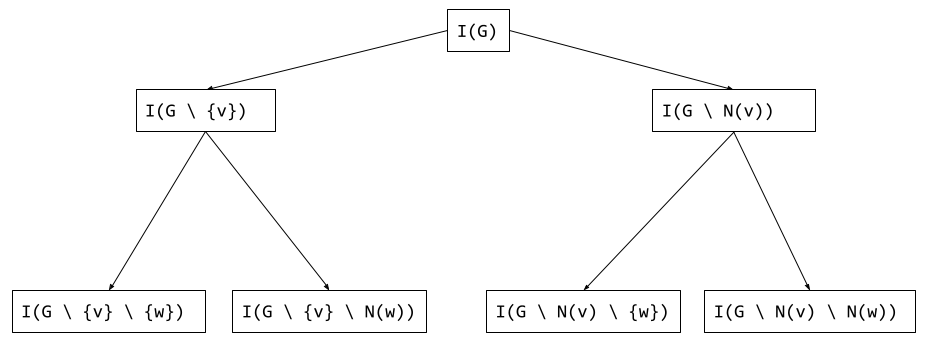
\includegraphics[scale=0.5]{assets/indep_set_sub.png}
\end{center}
Here, it's not hard to see that, if we continued generating this recursion tree, we see very little subproblem reuse. In other words, we end up with \emph{different subproblems} every time we get a new recursion. This is an issue for dynamic programming, as dynamic programming relies on subproblem reusability for efficiency.  

\bigskip 

In particular, for every subgraph $G'$, we need subproblems $I(G')$. But, we'll end up with $2^{|V|}$ subproblems; each vertex can either be in $G'$ or it can not be in $G'$. This further implies that the runtime of this algorithm will be exponential. 

\subsubsection{Hardness}
Maximum Independent Set of any general graph is what is known as an \textbf{NP-Hard} problem. Basically, this means that people believe that there may well be no \emph{efficient} algorithm for it (there is no sub-exponential runtime algorithm that solves this problem). 

\bigskip 

Instead, we now consider \emph{special cases} of this problem where we can do better. 

\subsubsection{Independent Sets and Components}
\begin{lemma}{}{}
    If $G$ has connected components $C_1, C_2, \dots, C_k$, then 
    \[I(G) = I(C_1) + I(C_2) + \dots + I(C_k)\]
\end{lemma}
\begin{mdframed}[]
    \begin{proof}
        Since the components don't connect to each other, an independent set for $G$ is exactly the union of an independent set for each of the $C_i$'s. THen, we can pick the biggest set for each $C_i$. 
    \end{proof}
\end{mdframed}

\subsubsection{Independent Sets of Trees}
One special case we can consider is independent sets of \emph{trees}. The reason why we look at trees is because, when we remove vertices from trees, it splits the tree up into disconnected subgraphs. This is useful as we can consider the disconnected subgraphs separately.
\begin{center}
    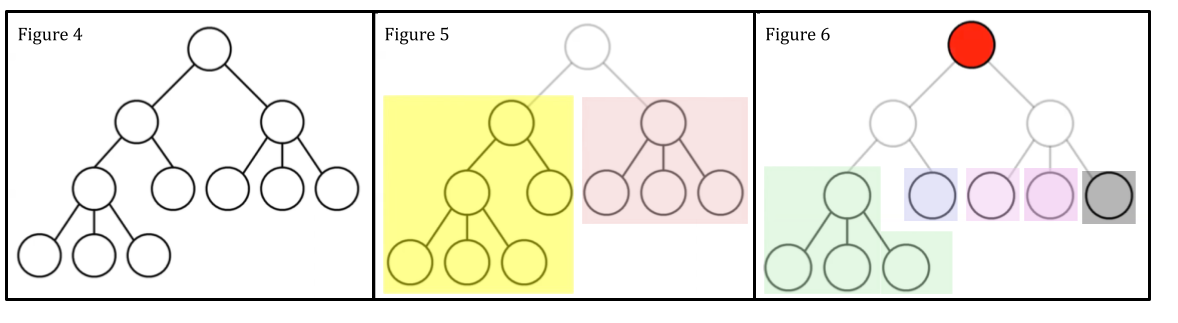
\includegraphics[scale=0.35]{assets/indep_set_tree.png}
\end{center}
Consider the above tree (Figure 4), and suppose we're focusing on the root of this tree $r$.
\begin{itemize}
    \item If we do \emph{not} include $r$ in our maximum independent set, then we want to look at the maximum independent sets of $G \setminus \{r\}$. For this, see Figure 5. 
    \item If we \emph{do} include $r$ in our maximum independent set, then we get $r$ for free, remove all of the neighbors of $r$, and then we can consider the remaining subgraphs. For this, see Figure 6. 
\end{itemize}
We note that the subproblems here are actually all \emph{sub-trees} of the original tree. If we look at a subtree of a subtree, we note that this is simply just another subtree. Then, it follows that the set of all problems that we need to solve is just the set of all possible subtrees of the original tree. 

\subsubsection{Recursion of the Tree}
We now consider several cases for our tree. 
\begin{itemize}
    \item Suppose the root is not used in the tree. Then, we end up with the subproblem of having to find the sum of the maximum independent sets of all of the children subtrees. That is, 
    \[I(G) = \sum I(\text{Children's Subtrees})\]
    This is shown by Figure 7 below.

    \item Suppose the root is used. Then, we end up with the subproblem of having to find the sum of all of the maximum independent sets of all of the grandchildren subtrees. That is, 
    \[I(G) = 1 + \sum I(\text{Grandchildren's Subtrees})\]
    This is shown by Figure 8 below.
\end{itemize}

\begin{center}
    \includegraphics[scale=0.4]{assets/indep_set_trees_2.png}

    \textbf{Note:} Triangles are arbitrary subtrees. 
\end{center}


\subsubsection{Example: Computing Maximum Independent Set of Trees}
Consider the following tree: 
\begin{center}
    \includegraphics[scale=0.3]{assets/ind_set_ex_tree.png}
\end{center}
Compute the maximum independent set. 

\begin{mdframed}[]
    Remember, our subproblems are the subtrees. So, for each node, we associate that node to the subproblem that corresponds to what is the maximum independent set of that node's subtree. The formula that we have is that this will always be the maximum of either: 
    \begin{itemize}
        \item The sum of the children's answers. 
        \item One more than the sum of the grandchildren's answers.
    \end{itemize}

    So, we start at the leaves and make our way up. 
    \begin{itemize}
        \item At the bottom level, each leaf (I, J, K, E, F, G, H) is going to have an answer of 1. If we just have that single node, the biggest independent set is going to be of size 1.
        \begin{center}
            \includegraphics[scale=0.2]{assets/indep_set_ex_1.png}
        \end{center}

        \item Consider node $D$. We can either take the sum of the children ($1 + 1 + 1 = 3$) or we can take one plus the sum of the grandchildren ($1 + 0 = 1$). Clearly, the sum of the children is the best option, so $D$ will be 3. 
        \begin{center}
            \includegraphics[scale=0.2]{assets/indep_set_ex_2.png}
        \end{center}
        Note that the children nodes are \emph{red} while node $D$ is \emph{green}.

        \item Consider node $B$. We can either take the sum of the children ($3 + 1 = 4$) or we can take one plus the sum of the grandchildren ($1 + (1 + 1 + 1) = 4$). Both options are good, so $B$ will be 4. 
        \begin{center}
            \includegraphics[scale=0.2]{assets/indep_set_ex_3.png}
        \end{center}
        Note that the children nodes are \emph{red}, the grandchildren nodes are \emph{blue}, and node $B$ is \emph{green}.

        \item Consider node $C$. We can either take the sum of the children ($1 + 1 + 1 = 3$) or we can take one plus the sum of the grandchildren ($1 + 0 = 1$). Clearly, the sum of the children is the best option, so $C$ will be 3. 
        \begin{center}
            \includegraphics[scale=0.2]{assets/indep_set_ex_4.png}
        \end{center}
        Note that the children nodes are \emph{red} and node $C$ is \emph{green}. Additionally, note that this is actually a subproblem that we've seen before.

        \item Consider node $A$. We can either take the sum of the children ($4 + 3 = 7$) or we can take one plus the sum of the grandchildren ($1 + (3 + 1 + 1 + 1 + 1) = 8$). Clearly, one plus the sum of the grandchildren is the best option, so $A$ will be 8. 
        \begin{center}
            \includegraphics[scale=0.2]{assets/indep_set_ex_5.png}
        \end{center}
        Note that the children nodes are \emph{red}, the grandchildren nodes are \emph{blue}, and node $A$ is \emph{green}.
    \end{itemize}
    Therefore, the maximum independent set of the \emph{whole tree} is \boxed{8}.
\end{mdframed}


\subsection{Problem: Traveling Salesman Problem}
\emph{In your job as a door-to-door vacuum salesperson, you need to plan a route that takes you through $n$ different cities. In order to space things out, you do not want to get back to the start until you have visited all cities. You also want to do so with as little travel as possible. }

\bigskip 

\textbf{Problem Statement:} Given a weighted (undirected) graph $G$ with $n$ vertices, find a cycle that visits each vertex exactly once whose total weight is as small as possible.


\subsubsection{Naive Algorithm}
The naive algorithm is to try all possible paths and see which is the cheapest. There are $n!$ paths; in particular, if we assume that we have a complete graph where all edges are there, then: 
\begin{itemize}
    \item There are $n$ possible options for the first city.
    \item There are $n - 1$ possible options for the second city. 
    \item There are $n - 2$ possible options for the third city. 
    \item \dots
\end{itemize}
This gives us $n(n - 1)(n - 2) \dots (2)(1) = n!$. Therefore, the runtime of the naive algorithm is approximately $\BigO(n!)$. 

\subsubsection{Problem Difficulty}
Like Maximum Independent Set, the Traveling Salesman Problem is widely considered to be a difficult problem. It is widely believed that there is no polynomial time algorithm for it. That being said, we note that there is an algorithm that beats the $n!$ naive algorithm.

\subsubsection{Setup}
We need to find some notion of \emph{partial solutions} for subproblems. In our case of cycles, we want to look for a path from vertex $s$ to $t$ such that, by adding one more vertex, we get a cycle. Therefore, the answer is given by 
\[\text{Best}_{st}(G) = \ell(s, t)\]
where $\text{Best}_{st}(G)$ is the best value of a path starting at vertex $s$ and ending at vertex $t$ that visits each vertex exactly once. 

\subsubsection{Recursion}
Suppose we have this path from $s$ to $t$. 
\begin{center}
    \includegraphics[scale=0.4]{assets/st_path_1.png}
\end{center}
We need to find some recursion that relates the answer to this problem to some kind of subproblem. The standard way to do this is to ask ourselves: what happens if we undo the last step? In our case, our last step is some edge from $u$ to $t$. That is: 
\begin{center}
    \includegraphics[scale=0.4]{assets/st_path_2.png}
\end{center}
The weight is, then, given by 
\[\ell(u, t) + \text{Length of Rest of Path}\]
We want the best path from $s$ to $u$ that uses every vertex \emph{except for $t$}. 
\begin{center}
    \includegraphics[scale=0.4]{assets/st_path_3.png}
\end{center}
Let's call this subproblem $\text{Best}_{su, -t}$; this is the minimum weight of the path from $s$ to $u$ that visits every vertex except for $t$ exactly once. Thus, the formula is given by 
\[\text{Best}_{st}(G) = \min_{u} \left(\text{Best}_{su, -t}(G) + \ell(u, t)\right)\]
For each $t$, we figure out what the best path is, add the length of the edge from $u$ to $t$, and then we take the minimum over all the possible vertices $u$ that have an edge to $t$. This will give us the best possible path length from $s$ to $t$. 

\subsubsection{Recursion II}
Now that we have a recursion that gives us the final answers in terms of subproblems, but we need a recursion that solves the subproblems. In other words, how do we solve for $\text{Best}_{su, -t}(G)$? 

\bigskip 

Again, we look at the edge from $v$ to $u$. We need the best path that connects $s$ to $v$ that uses all vertices except for $t$ and $u$. However, this makes the subproblems more complicated; all we're doing is avoiding more vertices. 

\bigskip 

Instead, we define $\text{Best}_{st, L}$ to be the best path length from $s$ to $t$ that uses exactly the vertices in $L$. That is, every vertex in $L$ shows up in the path exactly once. The rest of the vertices not in $L$ do not show up in the path. 

\bigskip 

The last edge is some $(v, t) \in E$ for some $v \in L$. Then, the cost of the path is given by 
\[\text{Best}_{sv, L \setminus \{t\}} + \ell(v, t)\]
So, the full recursion is given by 
\[\text{Best}_{st, L}(G) = \min_v \left(\text{Best}_{sv, L \setminus \{t\}}(G) + \ell(v, t)\right)\]

\subsubsection{Runtime Analysis}
Note that $L$ can be any subset of the vertices; thus, there are $2^n$ possibilities. Additionally, $s$ and $t$ can both be any vertices; thus, there are $n^2$ possibilities. Thus, there are $n^2 2^n$ subproblems. 

\bigskip 

We also need to check this for every $v$ (every vertex). This is because, for each subproblem, we need to find the minimum out of all vertices $v$. Thus, each subproblem takes $\BigO(n)$ time. 

\bigskip 

The final runtime is then given by $\BigO(n^3 2^n)$. 
















\newpage 
\section{NP-Completeness}
For almost every problem that we've seen in this class, there's a (usually bad) naive algorithm that just considers every possible answer and returns the best one. Some examples are: 
\begin{itemize}
    \item What is the shortest path from $s$ to $t$ in $G$? 
    \item What is the longest common subsequence? 
    \item What is the cloest pair of points? 
    \item Does $G$ have a topological ordering?
\end{itemize}
Of course, for nearly every algorithm we've discussed in class thus far, we were able to come up with a clever solution that runs in polynomial time. However, it's not generally the case that such (clever) algorithms will exist. 

\bigskip 

Note that, in this class, we define an \emph{easy} problem to be one that can be solved in polynomial time and a \emph{hard} problem to be one that cannot be solved in polynomial time. 

\subsection{Nondeterministic Polynomial (NP)}
Such problems are said to be in \textbf{Nondeterministic Polynomial} time (NP). To think of this in a theoretical perspective, imagine some nondeterministic computer that can try every possibility in parallel and then return the best possible solution. This type of computer can solve these problems in polynomial time. For example, it is allowed to search for the shortest path by trying every single path in \emph{parallel} and seeing which one is the shortest. There are two types of NP problems.
\begin{itemize}
    \item \textbf{NP-Decision} problems ask if there is some object that satisfies a polynomial time-checkable property. For example, is there a path from $s$ to $t$? If you write down a path from $s$ to $t$, then it is easy for the computer to check, in polynomial time, whether this is actually a valid path from $s$ to $t$. So, effectively, a decision problem is one whose answer is either \underline{yes} or \underline{no}.
    \item \textbf{NP-Optimization} problems ask for the object that maximizes (or minimizes) some polynomial time-computable objective. For example, instead of asking if there is a path from $s$ to $t$, you might instead ask what the shortest path from $s$ to $t$ is. So, effectively, an optimization problem is one whose answer is a minimum or maximum value. 
\end{itemize}
Essentially, $NP$ is the set of problems for which you can \emph{verify} the answer in polynomial time. Alternatively, it's the set of problems that can be solved in polynomial time by a \emph{nondeterministic} computer. 

\subsection{Difference Between Decision \& Optimization Problems}
% TODO expand on this
Now, note that NP-Decision and NP-Optimization problems are not too different. 
\begin{itemize}
    \item Every decision problem can be phrased as an optimization problem.
    \item Every optimization problem has a decision form.
\end{itemize}
For theoretical reasons, it's a good idea to understand the distinction. But, for practical purposes, it doesn't really matter. 

\subsection{Examples of NP Problems}
Some examples of NP problems are: 
\begin{itemize}
    \item Formula-SAT (NP-Decision). 
    \item Traveling Salesman Problem (NP-Optimization). 
    \item Hamiltonian Cycles (NP-Decision). 
    \item Generalized Knapsack (NP-Optimization). 
    \item Maximum Independent Set (NP-Optimization). 
\end{itemize}

\subsubsection{Formula-SAT}
Given a logical formula in a number of Boolean variables, is there an assignment to the variables that causes the formula to be true? 

\bigskip

For example, consider the following formulas: 
\begin{itemize}
    \item \underline{Formula 1:} If $x = \text{True}$, $y = \text{True}$, and $z = \text{False}$, then the following formula is satisfied: 
    \[(x \lor y) \land (y \lor z) \land (z \lor x) \land (\overline{x} \lor \overline{y} \lor \overline{z})\]

    \item \underline{Formula 2:} No assignments of $x$, $y$, and $z$ can satisfy the following formula: 
    \[(x \lor y) \land (y \lor z) \land (z \lor x) \land (\overline{x} \lor \overline{y}) \land (\overline{y} \lor \overline{z}) \land (\overline{x} \lor \overline{z})\]
\end{itemize}
There are some applications of SAT. In particular: 
\begin{itemize}
    \item \underline{Circuit Design:} Given some circuit, you want to make sure it actually computes the function that it's supposed to compute. This is basically a satisfiability problem.
    \item \underline{Logic Puzzle:} Most logic puzzle usually come down to some satisfiability problem; you want to find some settings or variables that satisfy some set of rules. 
\end{itemize}


\subsubsection{Hamiltonian Cycles}
Given an undirected graph $G$, is there a cycle that can visit every vertex exactly once? 

\subsubsection{General Knapsack}
\emph{Recall} that knapsack has a number of items, each with a weight and a value. The goal is to find the set of items whose total value is as much as possible without the total weight exceeding some capacity. 

\bigskip 

The general knapsack problem essentially runs in polynomial time in the \emph{weights}. Note that if the weights are allowed to be large (for example, written in binary), then you don't have a good algorithm. 


\subsection{Brute-Force Search}
Every NP problem has a brute-force search algorithm (the naive algorithm). In this class, we have looked at problems with algorithms that substantially improve on these brute-force algorithms. The question, then, is: \emph{does every NP problem have a better-than-brute-force algorithm?} Put it another way, \emph{is it the case that every algorithm in NP has a polynomial time algorithm?} 
\begin{itemize}
    \item If this is the case, then every NP problem has a reasonably efficient solution. No matter what kind of complicated search or decision problem we want to solve, there is always a clever way to do it better than brute-force. 
    \item If this is \emph{not} the case, then some NP problems are fundamentally difficult. There are some problems which are easy to check but there is no straight-forward or efficient way to actually find the answer.  
\end{itemize}
Note that $P$ is the set of all problems that can be solved in polynomial time. 

\subsection{Reductions}
In practice, at least some problems in NP appear to be hard. Despite decades of trying, people still don't know particularly good problems. Suppose you have a problem. How do you know if it's hard or not? 
\begin{itemize}
    \item You can search for an efficient algorithm to show that the problem is easy.
    \item You can try to prove that the problem is hard, but this is difficult. 
    \item You can try to relate the difficulty of your problem to the difficult of other problems.
\end{itemize}
With the last bullet point, we'll introduce the notion of \emph{reductions}. 

\subsubsection{What Is It?}
Reductions are a method for proving that one problem is \emph{at least as hard} as another problem. You can think of this as proving inequalities about problems. For example, problem $A$ is as hard as problem $B$. 

\bigskip 

The way we do this is as follows: we can show that \emph{if} there is an algorithm for solving $A$, then we can use this algorithm to solve $B$. Therefore, $B$ is no harder than $A$. 

\bigskip 

To better understand this concept, consider the following statements:
\begin{itemize}
    \item If problem $X$ is no harder than problem $Y$, and if $Y$ is easy, then $X$ must also be easy. 
    \begin{mdframed}[]
        To get the intuition behind this, suppose you have two numbers $x$ and $y$ such that $x$ is no greater than $y$; that is, $x \leq y$. Suppose $y$ is negative. Then, $x$ must also be negative (it cannot be positive). 

        \bigskip 

        The same idea holds here. If we have two problems $X$ and $Y$ such that $X$ is no harder than (or at least as easy as) $Y$ and $Y$ is easy, then $X$ cannot be harder than $Y$; $X$ has to be \emph{as easy as, or easier than,} $Y$. 
    \end{mdframed}
    \item If problem $X$ is no harder than problem $Y$, and if $X$ is hard, then $Y$ must also be hard. 
    \begin{mdframed}[]
        Again, to get the intuition behind this, suppose you have two numbers $x$ and $y$ such that $x$ is no greater than $y$; that is, $x \leq y$. Suppose $x$ is positive. Then, $y$ must also be positive (it cannot be negative). 

        \bigskip 

        The same idea holds here. If we have two problems $X$ and $Y$ such that $X$ is no harder than (or at least as easy as) $Y$ and $X$ is hard, then $Y$ cannot be easier than $X$; $Y$ has to be \emph{as hard as, or harder than,} $X$. 
    \end{mdframed}
\end{itemize}



\subsubsection{Reducing Hamiltonian Cycle to Traveling Salesman Problem}
We note that there is a natural reduction here. Particularly, they're related in the sense that we're visiting each vertex exactly once. 
\begin{itemize}
    \item Recall that the Traveling Salesman Problem asked: \emph{Given a weighted (undirected) graph $G$ with $n$ vertices, find a cycle that visits each vertex exactly once whose total weight is as small as possible.}
    \item Recall that the Hamiltonian Path problem asked: \emph{Given an undirected graph $G$, is there a cycle that can visit every vertex exactly once?}
\end{itemize}
To see this in action, consider the following example: 
\begin{center}
    \includegraphics[scale=0.4]{assets/ham_tsp.png}
\end{center}
Suppose we have an algorithm that solves the Traveling Salesman Problem efficiently. The idea is to convert a Hamiltonian Cycle problem to a Traveling Salesman problem. We do this by taking the original graph $G$ from the Hamiltonian Cycle problem and ``copying'' it to the Traveling Salesman problem, which we'll call the copied graph $H$. For all edges in $G$, we can give the corresponding edges in $H$ a weight of 1 (in Figure 1 and 2, the \emph{black} edges). Then, any extra edges that we add to $H$ (in Figure 2, the \emph{red} edges) can be given a very expensive weight (say 1000). 
\begin{center}
    \includegraphics[scale=0.4]{assets/ham_tsp_2.png}
\end{center}
Looking at Figure 4, we see that there is a Traveling Salesman path of cost 5. But, the path taken in the Traveling Salesman problem is the same path found in the Hamiltonian Cycle problem. So, the cheapest path we can hope for in the Traveling Salesman problem is the path consisting only of cost 1 edges. So, if we can find a path in the Traveling Salesman problem consisting only of cost 1 edges, then we have a Hamiltonian Cycle. \emph{Otherwise}, we'll have to make use of some expensive edges, so that implies that no such Hamiltonian Cycle can exist. 


\bigskip 

To be more formal about it, suppose you have a Hamiltonian Cycle instance $G$ with $n$ vertices. Suppose that you have an efficient algorithm $A$ that solves the Traveling Salesman Problem\footnote{We don't need to know how this algorithm works, only that you \emph{have} one.} Now, we create a Traveling Salesman problem instance $H$ where: 
\begin{itemize}
    \item The edges in $G$ have cost 1. 
    \item The edges not in $G$ have cost 1000 (or some expensive weight). 
\end{itemize}
Then, using this Traveling Salesman Problem algorithm, we can solve the Traveling Salesman instance. We note that we have a path of cost $n$ in $H$ if and only if there is a Hamiltonian cycle in $G$. Therefore, we can use this answer to solve the initial problem. 
\begin{itemize}
    \item If there is a Hamiltonian Cycle in $G$, then the Traveling Salesman Problem will have a weight of $n$. If there is \emph{no} Hamiltonian Cycle, then the best cost will be greater than $n$. 
    \item Any Traveling Salesman Problem that uses these expensive-costing edges will be more expensive than if we decided to use the edges with cost 1. 
    \item Therefore, we can run $A(H)$. If $A(H) \leq n$, then $G$ has a Hamiltonian cycle. Otherwise, it does not. 
\end{itemize}
From this, we get a new algorithm that can solve the Hamiltonian Cycle. This gives us a relation: the Hamiltonian Cycle problem is \emph{no harder} than the Traveling Salesman Problem. Now, since Hamiltonian Cycle is in NP, then it follows that the Traveling Salesman Problem must also be in NP. 

\bigskip 

So, what we've shown is that if we have an algorithm that can solve the Traveling Salesman problem, then we can turn that into an algorithm that solves the Hamiltonian Cycle path. 

\subsubsection{Generalization}
If we want to find a reduction from problem $A$ to problem $B$, then what we want to show is: 
\begin{itemize}
    \item If we are given an algorithm to solve that solves problem $B$, we can turn that into an algorithm that solves problem $A$. 
    \item Generally, we start with an instance of problem $A$. Then, with some polynomial time reduction algorithm, we can turn this instance of problem $A$ into an instance of problem $B$. Then, with a \emph{hypothetical} algorithm for problem $B$, we can find a solution to the problem $B$ instance. Then, we need to turn this solution of the problem $B$ instance into a solution for the problem $A$ instance; this is done by using a polynomial time interpretation algorithm. 
\end{itemize}
This process looks something like: 
\begin{center}
    \includegraphics[scale=0.4]{assets/reduction_cycle.png}
\end{center}
It's important that the reduction and interpretation algorithms run in \emph{polynomial time} by construction. If you have a polynomial time algorithm for problem $B$, then this entire process runs in polynomial time (i.e. you have a polynomial time algorithm for problem $A$). If you don't have a polynomial time algorithm for problem $B$, then there might be some other way to solve problem $A$, but you can't use this particular method. 

\bigskip 

So, effectively, if we have algorithms for reduction and interpretation, then: 
\begin{itemize}
    \item Given an algorithm to solve problem $B$, we can turn it into an algorithm to solve problem $A$. 
    \item This means that problem $A$ might be \emph{easier} to solve than problem $B$, but it cannot be \emph{harder}.
\end{itemize}

\subsection{Problem: Circuit SAT}
\textbf{Problem Statement:} Given a circuit $C$ with several Boolean inputs and one Boolean output, determine if there is a set of inputs that give the output \code{1}. 

\bigskip 

For example, the following circuit can be satisfied with inputs $x = y = z = 0$.
\begin{center}
    \includegraphics[scale=0.5]{assets/circuit_sat.png}
\end{center}

\subsubsection{Important Reduction}
Any NP-decision problem can be reduced to Circuit SAT. This is because any NP-decision problem is always of the same form; something is a NP-decision problem if it asks if there is some $X$ that satisfies a polynomial-time checkable property. 

\bigskip 

Essentially, for some polynomial-time computable function $F$, is there an $X$ such that $F(X) = 1$? We can create a circuit $C$ that computes $F$. Then, the problem is equivalent to asking if there is an input for which $C$ outputs 1. So, any NP-decision problem can be encoded as a Circuit SAT problem by taking the function that checks whether or not something satisfies your condition and encoding that as a Boolean circuit. 

\subsubsection{NP-Complete}
Circuit-SAT is our first example of an \textbf{NP-Complete} problem. This is a problem in NP that is at \emph{least} as hard as any other problem in NP. Therefore: 
\begin{itemize}
    \item If we can find a polynomial time algorithm that can solve Circuit SAT, we have a polynomial time algorithm for \emph{all} NP problems. 
    \item However, if any problem in NP is hard, then Circuit SAT is \emph{hard}.
\end{itemize}
\textbf{Remark:} Decision problems can be NP-Complete. For optimization problems, we call them NP-Hard.

\subsubsection{Other NP-Complete/Hard Problems}
We note that the following problems are all NP-Complete or NP-Hard: 
\begin{itemize}
    \item Formula SAT. 
    \item Maximum Independent Set. 
    \item Traveling Salesman Problem. 
    \item Hamiltonian Cycle. 
    \item Generalized Knapsack. 
\end{itemize}
We can show this by finding reductions from other NP-Hard or NP-Complete problems. 

\subsubsection{3-SAT}
3-SAT is a special case of formula-SAT where the formula is an \code{AND} of clauses and each clause is an \code{OR} of at most 3 variables or their negations. The following is an example of a 3-SAT problem: 
\[(x \lor y \lor z) \land (\overline{x} \lor u) \land (w \lor \overline{z} \lor u) \land (\overline{u} \lor w \lor \overline{z}) \land (\overline{y})\]
Here, each clause has \emph{at most three} variables or their negations. Each clause only has \code{OR} operations, and each clause is separated by \code{AND} operations. 

\subsubsection{Showing that 3-SAT is NP-Complete}
We will show that 3-SAT is NP-Complete. This is done by reducing Circuit-SAT to 3-SAT. 
\begin{itemize}
    \item Let's suppose we start with a circuit from a circuit-SAT problem. 
    \begin{center}
        \includegraphics[scale=0.4]{assets/circuit_sat.png}
    \end{center}

    \item Next, we'll create new variables for each outgoing wire.
    \begin{center}
        \includegraphics[scale=0.4]{assets/circuit_sat_2.png}
    \end{center}

    \item For each variable, we'll create a formula for each gate and for the output. We know that output $t$ must be true. Then, each clause is defined by its variables and the output after performing some operation (e.g. $x$ and $y$ are the inputs to the \code{AND} gate and $u$ is the output). Thus, we can write the formula out like so: 
    \[(v \iff y \lor z) \land (u \iff x \land y) \land (w \iff u \land v) \land (t \iff \overline{w}) \land t\]

    \item Note that the formula above is \emph{not} a 3-SAT formula. Effectively, we have 3-variable clauses that aren't 3-SAT clauses, so the goal is to write it in terms of them. 
    \begin{mdframed}[]
        To write thes 3-variable clauses in a way that represents 3-SAT clauses, we write out a truth table for each clause. Note that this is just an example of how you would do this.
        
        \bigskip 

        For example, consider a clause $(z \iff x \lor y)$. There are 8 different possibilities for all combinations of $x$, $y$, and $z$. For each combination of the original statement, we fill out the table like so. 
        \begin{center}
            \begin{tabular}{|c|c|c|c|}
                \hline 
                $x$ & $y$ & $z$ & $z \iff x \lor y$ \\ 
                \hline 
                0 & 0 & 0 & 1 \\ 
                0 & 0 & 1 & 0 \\ 
                0 & 1 & 0 & 0 \\ 
                0 & 1 & 1 & 1 \\ 
                1 & 0 & 0 & 0 \\ 
                1 & 0 & 1 & 1 \\ 
                1 & 1 & 0 & 0 \\ 
                1 & 1 & 1 & 1 \\ 
                \hline 
            \end{tabular}
        \end{center}
        We note that when we impose a 3-SAT clause on three variables, it excludes exactly \emph{one} combination of the inputs. We now describe how this works specifically. The idea is, given the original truth table of each clause:
        \begin{itemize}
            \item Find all rows where the result is \code{0}. In our initial example, we have 
            \begin{center}
                \begin{tabular}{|c|c|c|c|}
                    \hline 
                    $x$ & $y$ & $z$ & $z \iff x \lor y$ \\ 
                    \hline 
                    0 & 0 & 1 & 0 \\ 
                    0 & 1 & 0 & 0 \\ 
                    1 & 0 & 0 & 0 \\ 
                    1 & 1 & 0 & 0 \\ 
                    \hline 
                \end{tabular}
            \end{center}
    
            \item Then, for each row, negate the correct inputs so that the result would be \code{0} in the parameters; then, \code{OR} each of them. So, for example, with the first row, you would have $x \lor y \lor \overline{z}$. This is because $x$'s original value was \code{0}, so you would use $x$ in the 3-SAT instance to ``keep'' the \code{0}. Likewise, since $z$'s original value is \code{1}, you would use $\overline{z}$ to negate the \code{1} to a \code{0}. 
            \item For each of the remaining rows, do the same thing. Combine the clauses with an \code{AND} operator. For example, with the second row, we would have $x \lor \overline{y} \lor z$. Then, we can combine this with the previous step by using the \code{AND} operator like so: 
            \[(x \lor y \lor \overline{z}) \land (x \lor \overline{y} \lor z)\]
            Eventually, you'll end up with the 3-SAT-equivalent of the above expression:
            \[\underbrace{(x \lor y \lor \overline{z})}_{\text{1st Row}} \land \underbrace{(x \lor \overline{y} \lor z)}_{\text{2nd Row}} \land \underbrace{(\overline{x} \lor y \lor z)}_{\text{3rd Row}} \land \underbrace{(\overline{x} \lor \overline{y} \lor z)}_{\text{4th Row}} = (z \iff x \lor y)\]
            \item Repeat this process for each of the clauses that needs to be converted. 
        \end{itemize}
    \end{mdframed}

    \item This means that 3-SAT is also NP-Complete since any problem in NP can be reduced to Circuit-SAT, which in turn can be reduced to 3-SAT.
\end{itemize}

\subsubsection{Another Look at 3-SAT}
\begin{lemma}{}{}
    A 3-SAT instance is satisfiable if and only if it is possible to select one term from each clause without selecting both a variable and its negation. 
\end{lemma}

For example, suppose we have the 3-SAT instance 
\[(x \lor y \lor z) \land (\overline{x} \lor y) \land (\overline{y} \lor \overline{z}) \land (\overline{x} \lor z)\]
For each clause, suppose we select one of the terms like so.  
\[(x \lor \boxed{y} \lor z) \land (\boxed{\overline{x}} \lor y) \land (\overline{y} \lor \boxed{\overline{z}}) \land (\boxed{\overline{x}} \lor z)\]
We note that we did not select both a variable and its negation (e.g. we didn't select an $x$ and $\overline{x}$). This shows that this 3-SAT instance is satisfiable. For this example, if $x = \text{False}$, $y = \text{True}$, and $z = \text{False}$, then this statement will be \text{True}.

\begin{mdframed}[]
    \begin{proof}
        Suppose the instance was satisfiable. Then, at least one term in each clause must be true since each clause consists of \code{OR} of some number of terms. We select one such term from each clause. We note that they cannot contradict each other since all of those terms are consistent with the same satisfying assignment (it can't be true that $x$ was true in one clause and $\overline{x}$ was true in another clause because $x$ had to either be true or false).

        \bigskip 

        Suppose we have a 3-SAT instance where we can select one term from each clause without selecting both a variable and its negation. Suppose we set those clauses to be true (for example, we can set $x$ to be True and $y$ to be False or whatever so each clause is true). Then, we set the other variables arbitrarily since we know that at least one variable in each clause is true. This causes the whole statement to be true. 
    \end{proof}
\end{mdframed}

\subsubsection{Reducing 3-SAT to Maximum Independent Set}
This reduction is interesting especially since these problems appear to be unrelated. So, we start with a new formulation of 3-SAT. We want to select one term from each clause. We note that: 
\begin{itemize}
    \item For 3-SAT, we have a bunch of terms and we want to select some of them. 
    \item For MIS, we have a bunch of vertices and we want to select some of them. 
\end{itemize}
Suppose we want to reduce the following 3-SAT instance to a Maximum Independent Set instance.
\[(x \lor y \lor z) \land (\overline{x} \lor y) \land (\overline{y} \lor \overline{x})\]
This is how you would go about it. 
\begin{itemize}
    \item First, for each term in each clause, create a vertex.
    \begin{center}
        \includegraphics[scale=0.4]{assets/3sat_mis_1.png}
    \end{center}

    \item We now need to add edges in the following way. 
    \begin{itemize}
        \item First, we want to add edges between terms in the same clause.
        \begin{center}
            \includegraphics[scale=0.4]{assets/3sat_mis_2.png}
        \end{center}
        These edges ensure that, if we pick an independent set, we can only pick one term from each clause. 

        \item We add edges between contradictory terms.
        \begin{center}
            \includegraphics[scale=0.4]{assets/3sat_mis_3.png}
        \end{center}
        For example, we add an edge between the vertex $x$ and a vertex $\overline{x}$. 
    \end{itemize}
    This gives us the graph that we can use for the Maximum Independent Set instance. 
\end{itemize}

We note that an independent set in this graph has: 
\begin{itemize}
    \item At most one vertex from each clause. 
    \item No pair of vertices corresponding to contradictory terms. 
\end{itemize}
This is because of the edges; an independent set is not allowed to have two vertices connected by an edge. Since two things in the same clause are connected by an edge, it can't have two things in the same clause. And since two contradictory things are connected by an edge, it cannot have two contradictory things. Other than that, it can have whatever vertices it wants. 

\bigskip 

In particular, can we find an independent set such that its size is the same as the number of clauses in the original 3-SAT expression? If we can, then the only way to do that, since we can't select more than one vertex per clause, is if we pick exactly one vertex per clause. Additionally, because of the second contradict, we had to have done this without any pair that contradicts each other. This is exactly what we need to find a satisfying assignment for the 3-SAT. The opposite direction works as well; if we can satisfy the 3-SAT, we can pick one vertex from each clause and that will give us an independent set of the corresponding graph of the appropriate size. 

\bigskip 

So, to summarize the previous paragraph, we note that we have an independent set of size $c$ (where $c$ is the number of clauses) if and only if you can select one term from each clause without a contradicton. Therefore, the size of the maximum independent set is equal to the number of clauses if and only if the 3-SAT has a solution. 

\subsubsection{Example of Reducing 3-SAT to MIS}
Consider the graph we created in the previous section. If we select the following vertices (the pink vertices): 
\begin{center}
    \includegraphics[scale=0.4]{assets/3sat_mis_4.png}
\end{center}
Then, as long as $x = \text{False}$, $z = \text{True}$, and $y$ is arbitrary, then we found a satisfying assignment. 

\subsection{Problem: Zero-One Equations}
To prove more complicated reductions, it is helpful to have the correct problem to prove the reductions from. Sometimes, you might need to build intermediate problems that are nice to work with, mainly for convenience. 

\bigskip 

One convenient problem is the \textbf{zero-one equation}. Given a matrix $A$ with only \code{0}'s and \code{1}'s as entries and a vector $b$ of only \code{1}'s, determine whether or not there is an $x$ with \code{0} and \code{1} entries so that 
\[Ax = b\]
The problem is clearly in NP. We will show that is NP-complete. 

\subsubsection{Example: Zero-One Equations}
Find an $x_1, x_2, x_3$ such that 
\[\begin{bmatrix}
    1 & 0 & 1 \\ 1 & 1 & 0
\end{bmatrix} \begin{bmatrix}
    x_1 \\ x_2 \\ x_3
\end{bmatrix} = \begin{bmatrix}
    1 \\ 1
\end{bmatrix}\]
is satisfied. Equivalently, does there exist $x_1, x_2, x_3 \in \{0, 1\}$ such that 
\[\begin{cases}
    x_1 + x_3 = 1 \\ 
    x_1 + x_2 = 1
\end{cases}\]
holds? 

\begin{mdframed}[]
    It's not hard to see that this holds.     
\end{mdframed}

Generally, this is what a zero-one equation looks like; a bunch of sets of $x_i$'s that need to add to \code{1}. 

\subsubsection{Reducing 3-SAT to Zero-One Equation}
The idea behind reducing a 3-SAT formula to a zero-one equation is that we'll look at the formulation of 3-SAT and use one term from each clause. 

\bigskip 

We will create one variable for each term to denote whether or not it has been selected. Then, we'll add equations to enforce exactly one term from each clause such that no contradictory terms are selected. 

\bigskip 

To see this in action, we consider an example. Consider the following 3-SAT instance 
\[(\underbrace{x}_{x_1} \lor \overbrace{y}^{x_2} \lor \underbrace{z}_{x_3}) \land (\overbrace{\overline{x}}^{x_4} \lor \underbrace{y}_{x_5}) \land (\overbrace{\overline{y}}^{x_6} \lor \underbrace{\overline{x}}_{x_7})\]
\begin{itemize}
    \item We can translate this into the following zero-one equation instance by noting that we have one term per clause. That is: 
    \[\begin{cases}
        x_1 + x_2 + x_3 = 1 \\ 
        x_4 + x_5 = 1 \\ 
        x_6 + x_7 = 1
    \end{cases}\]
    \item We now want to make sure we don't select any contradictory terms. For example, we can't select both $x_1$ and $x_4$. So, if we use inequalities, we get something like: 
    \[\begin{cases}
        x_1 + x_4 \leq 1 \\ 
        x_1 + x_7 \leq 1 \\ 
        x_2 + x_6 \leq 1 \\ 
        x_5 + x_6 \leq 1
    \end{cases}\]
    So, if both $x_1$ and $x_4$ are \code{1}, then we have a problem. In any case, if we satisfy this system of inequalities of zero-one variables $x_1$ through $x_7$, then this is equivalent to having a solution to the original 3-SAT problem. 
    \item We note that we do not allow inequalities. A zero-one equation is only allowed to have \emph{equalities}. So, we need to tweak this system to make this equalities instead. An easy trick to do just this is to introduce a new variable. That is, if we had the inequality $a + b \leq 1$, then we can replace it with $a + b + c = 1$. The point is, if $a + b \leq 1$, then this will hold if and only if there is a zero-one variable $c$ such that $a + b + c = 1$. To see what we mean, we note that if $a + b = 0$, then we let $c = 1$; likewise, if $a + b = 1$, then $c = 0$. And, as usual, if $a + b = 2$, then we have an issue either way. 
    
    \bigskip 

    So, we have the system of \emph{equalities}: 
    \[\begin{cases}
        x_1 + x_4 + x_8 = 1 \\ 
        x_1 + x_7 + x_9 = 1 \\ 
        x_2 + x_6 + x_{10} = 1 \\ 
        x_5 + x_6 + x_{11} = 1
    \end{cases}\]
\end{itemize}
In general, the construction is as follows: 
\begin{itemize}
    \item Create one variable per term. 
    \item For each clause, create one equation. 
    \item For each pair of contradictory term, create an equation with those two and a new variable, and set that equal to one. 
\end{itemize}
This gives us a system of zero-one equations, which is satisfiable if and only if the original 3-SAT problem is. 

\subsubsection{Another Way of Looking at Zero-One Equations}
Suppose we treat $A$ as a bunch of column vectors. Recall that if $A = \begin{bmatrix}
    v_1 & v_2 & v_3 & \dots & v_n
\end{bmatrix}$, then we have 
\[Ax = x_1 v_1 + x_2 v_2 + \dots + x_n v_n\]
So, let's suppose we have the following matrix declaration 
\[A = \begin{bmatrix}
    1 & 0 & 1 \\ 0 & 0 & 1 \\ 0 & 1 & 1 \\ 1 & 1 & 0 
\end{bmatrix}\]
and we wanted to solve for $Ax = \vec{1}$. Then, we can write 
\[
    x_1 \begin{bmatrix}
        1 \\ 0 \\ 0 \\ 1
    \end{bmatrix} + x_2 \begin{bmatrix}
        0 \\ 0 \\ 1 \\ 1
    \end{bmatrix} + x_3 \begin{bmatrix}
        1 \\ 1 \\ 1\\ 0
    \end{bmatrix} = \begin{bmatrix}
        1 \\ 1 \\ 1 \\ 1
    \end{bmatrix}
\]
We can rewrite this like so 
\begin{equation*}
    \begin{aligned}
        &x_1 \begin{bmatrix}
            1 & 0 & 0 & 1
        \end{bmatrix} + \\ 
        &x_2 \begin{bmatrix}
            0 & 0 & 1 & 1
        \end{bmatrix} + \\ 
        &x_3 \begin{bmatrix}
            1 & 1 & 1 & 0
        \end{bmatrix} \\ 
        &= \begin{bmatrix}
            1 & 1 & 1 & 1
        \end{bmatrix}
    \end{aligned}
\end{equation*}
This is a bit suggestive because the way this was written implies that you could treat this as an addition of numbers. If we did this addition without performing any carries, this would almost be exactly the same computation as if we were adding numbers rather than adding vectors.

\bigskip 

Let's pretend we actually did addition of numbers. 
\begin{verbatim}
            x1 *    1 0 0 1     +
            x2 *    0 0 1 1     + 
            x3 *    1 1 1 0
            ---------------------
            =       1 1 1 1
\end{verbatim}
We have these three numbers and we want to see if there is some $x_1, x_2, x_3$ such that $x_1$ times the first number plus $x_2$ times the second number plus $x_3$ times the third number is equal to the solution. The only difference between adding numbers and adding vectors is that if we add numbers and we get big-enough terms, we might need to deal with carry-overs. For example, if we were doing base 2 addition, then we will get a carry over if we added 1 with 1. But, if we added these numbers in a high-enough base (e.g. base 10), we can't possibly get big-enough terms that will give us a carry over.

\bigskip 

So, if the numbers are represented in a large enough base (e.g. base 1000) that carrying is impossible, we have a solution to the vector equation if and only if we have a solution to the number equation. 


\subsection{Subset Sum}
What we just talked about actually relates naturally to the subset sum problem. 

\bigskip 

\textbf{Problem Statement:} Given a set $S$ of numbers and a target number $C$, is there a subset $T \subseteq S$ whose elements sum to $C$? 

\bigskip 

\textbf{Alternatively:} Can we find an $x_y \in \{0, 1\}$ such that 
\[\sum_{y \in S} x_y y = C\]
where
\[x_y = \begin{cases}
    0 & \text{If } y \text{ is not in the subset.} \\ 
    1 & \text{If } y \text{ is in the subset.} 
\end{cases}\]
Essentially, we want to find some setting of these binary variables so that the sum of all $y$ in the set of $x_y y$ is equal to the target. 

\subsubsection{Reducing Zero-One Equations to Subset Sum}
The alternative point that we've made can actually be used to relate the problem to zero-one equations. The idea is that we replace all of these vectors with numbers in base $n$ where $n$ is big enough so that there is no carry over with the arithmetic, and since the base is big enough that we'll never have to do any carry over, the vector addition problem is exactly equivalent to the number addition problem here. 

\bigskip 

Asking whether or not there is some zero-one linear combination of these numbers that add up to another number is equivalent to asking if there is a subset of these numbers which add up to the target. 

\bigskip 

So, starting from the instance of a zero-one equation, we can reduce the instance of subset sum with the same answer, which gives us the desired reduction. 

\bigskip 

Therefore, subset sum is NP-complete. 

\subsection{Generalized (Non-Repeated) Knapsack}
Subset sum is pretty closely related to the (non-repeated) knapsack. In particular: 
\begin{itemize}
    \item Subset sum wants to find a set of values so that the weights equal the capacity. 
    \item Knapsack wants to find a set of values so that the weights are at most the capacity and the value is as large as possible. 
\end{itemize}
There's a pretty easy way to get rid of this ``value'' idea. 

\subsubsection{Reducing Subset Sum to Knapsack}
We can reduce subset sum to knapsack in the following way. 
\begin{itemize}
    \item We create a knapsack problem where, for each item, the value of the item is just the weight of the item. Then, this becomes a ``the price is right'' knapsack; you want to find some set of items where the total weight is as large as possible without going over the capacity. 
    \item Maximizing the value is the same as maximizing the weight without going over the capacity. 
    \item We can, then, achieve a certain value (which is the capacity) if and only if there is a subset of the items with toatl weight equal to the capacity. So, if we want to answer the question ``is it possible to find a set of these items where the total weight is equal to the capacity?'' then this is exactly the same as the subset sum problem. 
\end{itemize}
So, this gives us a pretty natural reduction from subset sum to knapsack. Therefore, knapsack is NP-Hard. 

\subsubsection{Relation to Polynomial-Time Runtime Knapsack}
Our dynamic programming algorithm that we discussed some time ago was polynomial time in the \emph{total weight} (in terms of the numerical values of the weights). In this case, this is exponential. 


\subsection{Hamiltonian Cycles}
We want to show that Hamiltonian Cycles (and thus Traveling Salesman Problem) are NP-Complete (and NP-Hard). We will use a reduction from zero-one equations to Hamiltonian Cycles to show this. 

\subsubsection{Strategy}
Very often, to show that some problem is NP-Complete, we want to be able to show that it can simulate that logic somehow. This is difficuly for Hamiltonian Cycles as most graphs have too many options, so we will want to find specific graphs with clear, binary choices. 

\bigskip 

This is difficult for Hamiltonian cycle as most graphs have too many options in terms of the edges, so we want to find specific graphs with clear, binary choices. 

\bigskip 

To see how this would work, let's consider an example. 
\begin{itemize}
    \item First, start with a cycle. 
    \begin{center}
        \includegraphics[scale=0.35]{assets/zoe_ham_1.png}
    \end{center}
    There is clearly a Hamiltonian cycle here.

    \item Then, for some of these edges, we can double them up. That is, rather than 
    \begin{center}
        \includegraphics[scale=0.35]{assets/zoe_ham_2.png}
    \end{center}
    This graph still has a Hamiltonian cycle. But, now, there are multiple ways to find a Hamiltonian cycles (there are many binary choices that can be made here). At the moment, our construction has no constraints on these choices; we can pick whatever combinations of these binary choices we want and still get a Hamiltonian cycle. But, at least, we have a prototype of a graph where trying to find a Hamiltonian cycle on this graph involves making a specific collection of (in this case) binary choices, which is a good place to start if we want to make some NP-Completeness reductions. Now, at least, there is some \emph{logic} involved. We just need to add some limitations as to what choices we can make. 

    \bigskip 

    So, to sumamrize, in our cycle, we must pick one edge from each pair, which provides a nice set of binary variables. 

    \item We need to add restrictions so that we can't just use any collection of choices. We need to make it difficult to figure out whether it is possible to make the right choices or not. To do so, we make use of a \emph{gadget}. 
    \begin{center}
        \includegraphics[scale=0.35]{assets/zoe_ham_3.png}
    \end{center}
    Gadgets are generally useful for proving NP-Completeness/Hardness reduction problems. It's not necessarily well-defined; it's essentially just a piece of construction which only has a few ways it can be filled out. It often allows us to enforce some condition or simulate some more complicated behavior. So, in our case here, this gadget will be a subgraph of the full graph we made. We have a collection of edges and vertices, and there are these four edges with arrows which connects the gadget to the rest of the graph.
    
    \bigskip 

    If this gadget is part of the graph and there is a Hamiltonian cycle in this graph, then we note that, because of these degree 2 vertices, any Hamiltonian cycle has to visit these vertices. The only way it can do that is if it uses both edges on each of the columns (the red edges below).
    \begin{center}
        \includegraphics[scale=0.35]{assets/zoe_ham_4.png}
    \end{center}

    When we get to the top or bottom of one of these columns, the vertex at the top or bottom of the columns has to connect to exactly one of its left or right neighboring vertices. We can't just connect these vertices however we want, or else we might have a disconnected cycle in the middle. 

    \bigskip 

    There are only two ways to fill these edges out and still be consistent with having a Hamiltonian cycle; both of those ways involve a zig-zag pattern (see the two graphs below). 
    \begin{center}
        \includegraphics[scale=0.3]{assets/zoe_ham_5.png}
        \includegraphics[scale=0.3]{assets/zoe_ham_6.png}
    \end{center}
    To see how this gadget used, suppose we have a giant cycle, and in the middle of this cycle we have these two binary choices that can be made. 
    \begin{center}
        \includegraphics[scale=0.35]{assets/zoe_ham_7.png}
    \end{center}
    We can then hook the gadget up between these pair of edges. 
    \begin{center}
        \includegraphics[scale=0.35]{assets/zoe_ham_8.png}
    \end{center}
    There are two ways to fill out ths gadget.
    \begin{center}
        \includegraphics[scale=0.30]{assets/zoe_ham_9.png}
        \includegraphics[scale=0.30]{assets/zoe_ham_10.png}
    \end{center}
    This allows us to force logic upon our choices. By doing this for several pairs of edges, we can construct a Hamiltonian cycle problem equivalent to the following:  
    \begin{itemize}
        \item You are given a number of choices where you need to pick one from several options (of multi-edges). 
        \item You have several constraints that say that of the two choices you could make, you must have picked exactly one of them. 
    \end{itemize}
    With this in mind, we want to see if you can simulate a hard problem from this. 
\end{itemize}
Now, we can talk about the zero-one equation. 
\begin{itemize}
    \item For each variable, choose either 0 or 1. This will tell you the value of that variable.
    \item For each equation, choose one variable to be equal to 1.
    \item We also need to add some constraints. For each variable that appears in an equation, exactly one of the following should be selected. Either that variable is in the equation, or that variable is equal to 0. 
\end{itemize}

\subsubsection{Example: Zero-One Equation}
Suppose you have the following zero-one equation 
\[\begin{cases}
    x_1 + x_2 + x_3 = 1 \\ 
    x_2 + x_4 = 1
\end{cases}\]

First, we can build a graph for each gadget. 
\begin{center}
    \includegraphics[scale=0.30]{assets/zoe_ham_12.png}
\end{center} 
For each variable that appears in each equation, we have a gadget which enforces the constraint that we either select a variable or we set that variable equal to 0. 
\begin{center}
    \includegraphics[scale=0.30]{assets/zoe_ham_11.png}
\end{center} 
To see what this means, consider the top gadget. This is saying that either: 
\begin{itemize}
    \item Either $x_2$ will be selected from the equation. 
    \item Or we set $x_2$ equal to 0. 
\end{itemize}
This gives us a complicated Hamiltonian cycle problem, but this graph that we built has a Hamiltonian cycle if and only if the corresponding zero-one equation has a solution. Consider the following: 
\begin{center}
    \includegraphics[scale=0.3]{assets/zoe_ham_13.png}
\end{center}
Here, we are saying that $x_1 = 1$, $x_2 = x_3 = 0$, and $x_4 = 1$. 

\subsection{Reduction Summary}
\begin{center}
    \includegraphics[scale=0.3]{assets/reduction_summary.png}
\end{center}






















\newpage 
\section{Dealing with NP-Completeness}
We now talk about how to deal with NP-Completeness. First, before solving a problem, we want to see if the problem is NP-Complete. If the problem is, then we probably won't find a very good solution for it. So, at least, you have an excuse for not having a better algorithm. However, if you need to solve the problem, well, you still need to find some way to solve it. In this section, we'll briefly talk about ways to solve such problems. 

\bigskip 

Consider the following statement: \emph{if your problem is NP-Hard/NP-Complete, then unless $P = NP$, there is no algorithm that gives the exact answer to your problem on all instances in polynomial time.} Despite not being able to get around the fact that you might not be able to solve such problems efficiently, there are loopholes in this statement that can be exploted.
\begin{itemize}
    \item ``\textbf{all instances}'': there are worst-case instances which can be very hard to solve. But, the instances that you're working on is easier. For example, maximum independent set is a hard problem, but maximum independent set of trees is not. So, see if you can make further assumptions. 
    \item ``\textbf{exact answer}'': you sometimes do not need the \emph{best} answer. It's okay to have a good answer. This leads to the notion of approximation algorithms. 
    \item ``\textbf{polynomial time}'': for finite input sizes, or smaller input sizes, the runtime of your algorithm might not matter. So, an \emph{efficient brute-force} algorithm might be good enough. 
    \item ``\textbf{P = NP}'': If you can prove that $P = NP$, then you can solve whatever problems you would like in $NP$. 
\end{itemize}

\subsection{Sudoku}
Consider the logic puzzle Sudoku, where you have a $9 \times 9$ grid of numbers with 1 - 9 so that:
\begin{itemize}
    \item Each row has all numbers. 
    \item Each column has all numbers. 
    \item Each of the main $3 \times 3$ sub-squares has all numbers. 
    \item Some entries are pre-filled. 
\end{itemize}
For a fixed board size, you can't really say that this problem is in NP. However, there is an obvious generalization which is formally a NP-Hard problem. 

\subsubsection{Brute-Force}
Generally speaking, you cannot do much better than brute-force saerch. However, we note that, even for a fixed board size of $9 \times 9$, a brute-force search would consider $9^{81}$ possibilities. This would essentially take longer than the lifespan of the universe. However, people can solve them while waiting for something. How is this the case? 

\subsubsection{Deductions}
One way to make progress is to make deducations. In particular: 
\begin{itemize}
    \item We can use the rules to show that some square can only be filled out in one way. 
    \item We can use that information to help fill out more squares. 
    \item If you're lucky, you can keep going until the entire problem is solved. 
\end{itemize}
To see an example of how this would work, consider the 3-SAT problem $x \land (\overline{x} \lor y) \land (\overline{x} \lor \overline{y} \lor z)$. 
\begin{itemize}
    \item For the whole statement to be true, each clause must be true. So, $x = \text{True}$.
    \item If we simplify this, we now get $y \land (\overline{y} \lor z)$. Therefore, $y = \text{True}$. 
    \item Simplifying this further gives us $z$. Therefore, $z = \text{True}$. 
\end{itemize}
So, instead of having to check every possible options, we can just make a sequence of logical deductions which led us to the answer. 

\subsubsection{Getting Stuck}
If we just have simple rules like this, we'll get stuck pretty quickly. This especially applies if you have harder problems. So, how do you get unstuck? 
\begin{itemize}
    \item Use stronger deduction rules. In the case of Sudoku:
    \begin{itemize}
        \item Find a square that only one number can fill.
        \item Find a region with only one place for a given number to be put. 
        \item Find a pair of squares in the same row that must contain two numbers (which then cannot appear elsewhere in that row).
        \item Find a rectangle whose corners must contain 2 copies of a number. That number cannot appear elsewhere in those rows/columns.
        \item Find 3 rows and 3 columns whose intersections must contain 3 copies of a number. That number cannot appear elsewhere in those rows and columns.
    \end{itemize}
    This helps cuts down a bunch of possibilities which can simplify your search space. 

    \item Guess and check. For example, you can make a guess, and then use the deduction rules to see if you can reach a contradiction. If you reach a contradiction, then you know that the guess you made is wrong so you can guess again. Formally, this is known as \emph{backtracking}.
\end{itemize}

\subsection{Finding Exact Solutions to NP-Complete/Hard Problems}
There are two strategies to find exact solutions. 

\subsubsection{Backtracking}
The idea behind backtracking is as follows. 
\begin{verbatim}
    Search(Problem P, Search Space S):
        If you can find a contradiction:
            return 'no solution' 
        Split S into subproblems S1, S2, ... 
        For each i: 
            Run Backtracking(P, Si)
        Return any solutions found. 
\end{verbatim}
Essentially, the idea is to try every possible solution in $S$. However, if we can reach a contradiction -- especially early on -- then we can cut our search space by a significant factor. 

\bigskip 

Another thing to consider is how you split your search space. Generally, you want to branch on variables that have a lot of deductive power -- essentially, variables which may lead to a contradiction very early on. 

\bigskip 

Note that backtracking works well for decision problems. However, for optimization problems, not so much. So, we introduce the idea of \emph{branch and bound}.

\subsubsection{Branch and Bound}
For optimization problems, we need to keep track of the best solutions so far. Then, instead of a contradiction, what you need to do is \emph{bound} the best solution in $S$ (the space you're searching over). Then, if it's \emph{worse} than the best so far, then stop. 

\bigskip 

Essentially, the idea is as follows. 
\begin{verbatim}
    BranchAndBound(Best, Search Space S):
        If UpperBound(S) <= Best:
            Return 'no improvement' 
        If S is a full solution: 
            Return value of S 
        Split S into subproblems S1, S2, ... 
        For each i: 
            New = BranchAndBound(Best, Si)
            Best = Max(New, Best)
        Return Best 
\end{verbatim}


\subsection{Heuristic Search}
Heuristic search is this idea where we relax one of the rules to find an answer. For example, we can relax the rule that we want the exact answer. Often times, especially for optimization problems, we don't necessarily need the best answer; we only need a ``good enough'' answer. 

\subsubsection{Hill-Climbing}
The high-level idea is what is known as \emph{hill-climbing}. The idea is that we find $x$, and then we try all $y$ near $x$. If $f(y) > f(x)$, then we set $x$ to be $y$. This idea would be repeated until you don't really see an improvement. 

\subsubsection{Getting Stuck}
An issue is that you can get stuck, though. For example, suppose you're at the bottom of a hill. There are going to be a lot of local maximum points, which your algorithm might interpret as the maximum. However, we note that there could very well be an absolute maximum point that the algorithm can't find. 

\subsubsection{Getting Unstuck}
There are several ways to get unstuck. 
\begin{itemize}
    \item Randomized Restart: If you try many starting points, you might be able to find the one that is the true maximum. In the hill-climbing analogy, this just means starting at different points in the hill. 
    \item Expand Search Area: Instead of looking for changes in a small, restricted area, you could expand how far you saerch to hopefully find a better answer. The disadvantage of this is that the larger areas could take more work. However, at least it's harder to get stuck. In the hill-climbing analogy, this means that, rather than taking one step to see if you can find a higher point, you could take multiple steps around. 
    \item Simulated Annealing: At the start of the algorithm, you can take big, random steps. This will hopefully get you to the right hill. Then, as the algorithm progresses, the step distance decreases and the algorithm starts to fine-tune more precisely. This works well, in practice, for a number of problems. 
\end{itemize}
In either case, it's still no guarantee of finding the actual maximum in polynomial time. 


\subsection{Approximation Algorithms}
An $\alpha$-approximation algorithm is an algorithm that always obtains the optimal value up to a factor of $\alpha$. 

\bigskip 

For example, a 2-approximation algorithm is an algorithm that obtains the optimal value up to a factor of 2; if you're maximizing, you're at least a half of the maximum value, and if you're minimizing, you're at most twice of the optimal value. 

\bigskip 

An approximation answer doesn't necessarily give you the best answer, but at least it gives you some rigorously proven guarantees about how good your answer is. 


\subsubsection{Problem: Vertex Cover}
Given a graph $G$, find a set $S$ of vertices so that every edge of $G$ contains a vertex of $S$ and so that $|S|$ is as small as possible. 

\bigskip 

For example, consider the graph below.
\begin{center}
    \includegraphics[scale=0.5]{assets/vertex_cov.png}
\end{center}
The minimal size is 3, and is given by: 
\begin{center}
    \includegraphics[scale=0.5]{assets/vertex_cov_2.png}
\end{center}

\subsubsection{Greedy Algorithm for Vertex Cover}
The greedy algorithm for the vertex cover problem is as follows: 
\begin{verbatim}
    GreedyVertexCover(G):
        S = {}
        While S doesn't cover G:
            (u, v) = some uncovered edge 
            Add u and v to S
        Return S
\end{verbatim}
We note that this is a 2-approximation algorithm. 

\subsubsection{Example of Algorithm on Graph}
In the graph above, we note that this algorithm could potentially find the following vertices:
\begin{center}
    \includegraphics[scale=0.5]{assets/vertex_cov_3.png}
\end{center}
The algorithm finds $k$ edges and returns $2k$ vertices. These edges are vertex-disjoint, i.e. no two edges could share a vertex since we added both vertices whenever we account for an edge. So, any cover must have at least one vertex on each of these edges. So, the optimal cover has size at least $k$, but we have one of $2k$. 

\end{document}